\documentclass{article}

\usepackage[pdftex]{hyperref}
\usepackage{graphicx}
\usepackage{listings,listings-rust}
\usepackage[T1]{fontenc}
\usepackage{ae,aecompl}
\usepackage[scaled]{luximono}
\usepackage{array}
\usepackage{tikz}
\usepackage{marvosym}

\newcommand{\poison}{\textrm{\Biohazard}}

\DeclareMathAlphabet{\mathsfsl}{OT1}{cmss}{m}{sl}

\usetikzlibrary{arrows,shapes,snakes,automata,backgrounds,petri,positioning}

\tikzstyle{place}=[circle,draw,minimum size=5mm]
% -> Uses trick from http://tex.stackexchange.com/a/170207
\tikzstyle{transitionV}=[rectangle,thick,fill=black,minimum width=5mm,
    inner ysep=1pt]
\tikzstyle{transitionH}=[rectangle,thick,fill=black,minimum height=5mm,
    inner xsep=1pt]
\tikzstyle{every picture}+=[node distance=0.75cm,>=stealth',auto]

\tikzset{
    state/.style={
           rectangle,
           draw=black
           },
}

\addtolength{\hoffset}{-2cm}
\addtolength{\textwidth}{4cm}
\addtolength{\voffset}{-2cm}
\addtolength{\textheight}{3cm}

%\lstset{language=c,columns=fullflexible,basicstyle=\ttfamily,identifierstyle=\itshape} %,literate={&*&}{{$\mathrm{{\&}{*}{\&}}$}}1}
\lstset{language=Rust,columns=fullflexible,basicstyle=\ttfamily} %,literate={&*&}{{$\mathrm{{\&}{*}{\&}}$}}1}
\lstset{moredelim=**[s][\itshape]{/*}{*/},moredelim=**[l][\itshape]{//},morekeywords={req,ens,true,false,pred,lem,fix,pred_ctor,leak,open,close,bool,inv,inductive,assert,pred_fam,pred_fam_inst,fn_type,produce_fn_ptr_chunk}}

\newtheorem{exercise}{Exercise}

\title{Verifying purely \texttt{unsafe} Rust programs with VeriFast: a tutorial}

\author{Bart Jacobs\\
{\small KU Leuven, Department of Computer Science, DistriNet Research Group}}

\begin{document}

\maketitle

\setcounter{tocdepth}{1}
\tableofcontents

\newpage

\section{Introduction}

VeriFast is a tool for verifying the absence of undefined behavior\footnote{\url{https://doc.rust-lang.org/reference/behavior-considered-undefined.html}} in single-threaded and multithreaded Rust\footnote{VeriFast also supports C and Java. See \emph{The VeriFast Program Verifier: A Tutorial} and \emph{VeriFast for Java: A Tutorial}.}
programs that use \lstinline|unsafe| blocks. The tool reads an
\verb|.rs| source code file and reports either ``0 errors found'' or
indicates the location of a potential error. If the tool
reports ``0 errors found'', this means\footnote{There are a few
known reasons (known as \emph{unsoundnesses}) why the tool may
sometimes incorrectly report ``0 errors found''; see \textsf{soundness.md} and \textsf{tests/rust/README.md} at \textsf{https://github.com/verifast/verifast} and \url{https://github.com/verifast/verifast/issues?q=is\%3Aissue\%20state\%3Aopen\%20label\%3Aunsoundness}. There
may also be unknown unsoundnesses.} that the program
\begin{itemize}
\item does not perform illegal memory accesses, such as reading or
    writing a struct instance field after the struct instance has been
    deallocated, or reading or writing beyond the end of an array (known as
    a \emph{buffer overflow}, the most common cause of security
    vulnerabilities in operating systems and internet services) and
\item does not include a certain type of concurrency errors known as
    \emph{data races}, i.e.~unsynchronized conflicting accesses of the
    same field by multiple threads. Accesses are considered
    conflicting if at least one of them is a write access. And
\item complies with function preconditions and
    postconditions specified by the programmer in the form
    of special comments (known as \emph{annotations}) in
    the source code.
\end{itemize}

Many errors in Rust programs that use \lstinline|unsafe| blocks, such as illegal memory accesses and
data races, are generally very difficult to detect by
conventional means such as testing or code review, since they
are often subtle and typically do not cause a clean crash but
have unpredictable effects that are difficult to diagnose.
However, even many security-critical and safety-critical Rust programs,
such as operating systems, device drivers, web servers (that
may serve e-commerce or e-banking applications), embedded
software for automobiles, airplanes, space applications,
nuclear and chemical plants, etc.\ use \lstinline|unsafe| blocks, where
these programming errors may enable cyber-attacks or cause
injuries. For such programs, formal verification approaches
such as VeriFast may be the most effective way to achieve the
desired level of reliability.

To detect all errors, VeriFast performs \emph{modular symbolic execution}
of the program. In particular, VeriFast symbolically executes the body of
each function of the program, starting from the symbolic state described
by the function's precondition, checking that \emph{permissions} are
present in the symbolic state for each memory location accessed by a
statement, updating the symbolic state to take into account each
statement's effect, and checking, whenever the function returns, that the
final symbolic state satisfies the function's postcondition. A symbolic
state consists of a \emph{symbolic heap}, containing permissions (known as
\emph{chunks}) for accessing certain memory locations, a \emph{symbolic
store}, assigning a symbolic value to each local variable, and a
\emph{path condition}, which is the set of \emph{assumptions} about the
values of the \emph{symbols} used in the symbolic state on the current
execution path. Symbolic execution always terminates, because thanks to
the use of loop invariants each loop body needs to be symbolically
executed only once, and symbolically executing a function call uses only
the function's precondition and postcondition, not its body.

We will now proceed to introduce the tool's features step by
step. To try the examples and exercises in this tutorial
yourself, please download the release from the VeriFast website
at
\begin{center}
\texttt{https://github.com/verifast/verifast}
\end{center}
. You will find in the \texttt{bin} directory a command-line version of
the tool (\texttt{verifast.exe}), and a version that presents a graphical
user interface (\texttt{vfide.exe}).

Throughout this tutorial, you will find exercises that ask you to annotate a small Rust program so that it is accepted by VeriFast. You can find solutions to all exercises at the end of this tutorial. Furthermore, un-annotated and annotated versions of each solution are included in the VeriFast distribution in directories \verb|rust_tutorials/unsafe/problems| and \verb|rust_tutorials/unsafe/solutions|, respectively.

\section{Example: illegal\_access.rs}

To illustrate how VeriFast can be used to detect programming
errors that are difficult to spot through testing or code
review, we start by applying the tool to a very simple Rust
program that contains a subtle error.

Please start \texttt{vfide.exe} with the \texttt{illegal\_access.rs}
program that can be downloaded from
\begin{center}
\texttt{https://www.cs.kuleuven.be/\symbol{126}bartj/verifast/illegal\_access.rs}
\end{center}
. The program will be shown in the VeriFast IDE. To verify the program,
choose the \textbf{Verify program} command in the \textbf{Verify} menu,
press the \textbf{Play} toolbar button, or press F5. You will see
something like Fig~\ref{figure:illegal-access1}.
\begin{figure}
\begin{center}
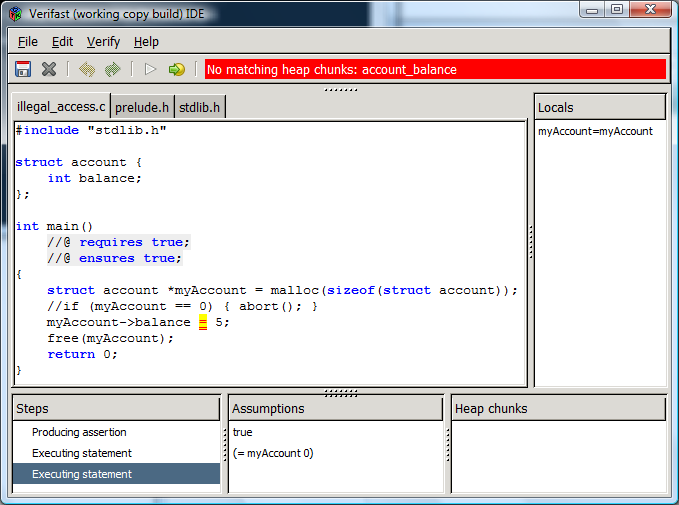
\includegraphics[width=12cm]{illegal_access.png}
\end{center}
\caption{A screenshot of \texttt{illegal\_access.rs} in the VeriFast IDE}\label{figure:illegal-access1}
\end{figure}
The program attempts to access the field \lstinline|balance| of the struct
instance \lstinline|my_account| allocated using \lstinline|alloc|. However,
if there is insufficient memory, \lstinline|alloc| returns a null pointer and no
memory is allocated. VeriFast detects the illegal memory access that
happens in this case. Notice the following GUI elements:
\begin{itemize}
\item The erroneous program element is displayed in a red
    color with a double underline.
\item The error message states: ``No matching heap chunks: $\mathsf{Account\_balance\_(my\_account, \_)}$''. Indeed, in the scenario where there
    is insufficient memory, the memory location (or
    \emph{heap chunk}) that the program attempts to access
    is not accessible to the program.
    $\mathsf{Account\_balance\_}$ is the type of heap chunk
    that represents the (possibly uninitialized) $\mathsf{balance}$ field of the
    instance of struct $\mathsf{Account}$ pointed to by pointer $\mathsf{my\_account}$.
\item The assignment statement is shown on a yellow
    background. This is because the assignment statement is
    the \emph{current step}. VeriFast verifies each
    function by stepping through it, while keeping track of
    a symbolic representation of the relevant program
    state. You can inspect the symbolic state at each step
    by selecting the step in the Steps pane in the lower
    left corner of the VeriFast window. The program element
    corresponding to the current step is shown on a yellow
    background. The symbolic state consists of the
    \emph{path condition}, shown in the Assumptions pane;
    the \emph{symbolic heap}, shown in the Heap chunks
    pane; and the \emph{symbolic store}, shown in the
    Locals pane.
\end{itemize}

To correct the error, uncomment the commented statement. Now
press F5 again. We get a green bar: the program now verifies. This means VeriFast has symbolically executed all possible paths of execution through function \lstinline|main|, and found no errors.

Let's take a closer look at how VeriFast symbolically executed this function. After VeriFast has symbolically executed a program, you can view the \emph{symbolic execution tree} for each function in the Trees pane. The Trees pane is hidden by default, but you can reveal it by dragging the right-hand border of the VeriFast window to the left. At the top of the Trees pane is a drop-down list of all functions that have been symbolically executed. Select the \textsf{Verifying function '\lstinline|main|'} item to view the symbolic execution tree for function \lstinline|main|.

A symbolic execution tree has four kinds of nodes:
\begin{itemize}
\item The \emph{top node} represents the start of the symbolic execution. Click the top node: in the initial symbolic execution state, there are no heap chunks (the Heap chunks pane is empty), there are no local variables (the Locals pane is empty), and there are no assumptions (the Assumptions pane is empty).
\item There is one \emph{fork node} at each point where a symbolic execution path forks into two paths. This happens when multiple cases need to be considered in the symbolic execution; it is therefore also called a \emph{case split}. The symbolic execution of function \lstinline|main| involves three case splits: the first case split is where symbolic execution of the \lstinline|alloc| call forks into one branch where no memory is available and therefore \lstinline|alloc| returns a null pointer, and another branch where memory is available and therefore \lstinline|alloc| allocates the requested amount of memory and returns a pointer to it. A case split also happens on each of these branches when symbolically executing the \lstinline|if| statement.
\item A black \emph{final node} is shown for the final symbolic execution state on each path where additional symbolic execution steps were performed after the last fork. This is the case for one of the branches of each of the two fork nodes corresponding to the \lstinline|if| statement.
\item There is one green \emph{leaf node} at the end of each complete symbolic execution path through the function. Click the black node preceding any leaf node to see the full corresponding symbolic execution path in the Steps pane.
Function \lstinline|main| has four symbolic execution paths: two paths end when the \lstinline|if| branch is detected to be inconsistent with the preceding \lstinline|alloc| branch; one path where no memory is available ends when the program ends due to the call of \lstinline|handle_alloc_error|; and a fourth path, where memory is available, ends when the function returns.
\end{itemize}

Click the black node preceding the rightmost leaf node to view the (feasible) execution path where \lstinline|alloc| successfully allocates memory. Notice that VeriFast shows arrows in the left margin next to the code of function \lstinline|main| to indicate that this path executes the second case of the \lstinline|alloc| statement and the second case of the \lstinline|if| statement.

To better understand the details of VeriFast's symbolic execution, we will step through this path from the top. Select the first step in the Steps pane. Then, press the Down arrow key. The \textsf{Verifying function \lstinline|main|} step does not affect the symbolic state. The \textsf{Producing assertion} step adds the assumption \textsf{true} to the Assumptions. We will consider production and consumption of assertions in detail later in this tutorial. We now arrive at the \textsf{Executing statement} step for the \lstinline|alloc| statement. This statement's effect takes place in the next step, the \textsf{Executing second branch} step; it affects the symbolic state in three ways:
\begin{itemize}
\item It adds the heap chunks $\mathsf{Account\_balance\_}(\mathsf{my\_account}, \mathsf{dummy})$ and $\mathsf{alloc\_block\_Account}(\mathsf{my\_account})$ to the symbolic heap (as shown in the Heap chunks pane). Here, $\mathsf{my\_account}$ and $\mathsf{dummy}$ are \emph{symbols} that represent unknown values. Specifically, $\mathsf{my\_account}$ represents a pointer to the newly allocated struct instance, and $\mathsf{dummy}$ represents the initial state of the \lstinline|balance| field of the struct instance. (The initial state of memory allocated using \lstinline|alloc| is unspecified, unlike in Java where the fields of a new object are initialized to the default value of their type. In fact, in Rust, uninitialized memory might be in a special \emph{poisoned} state whose behavior is different from any initialized state.\footnote{See \url{https://www.ralfj.de/blog/2019/07/14/uninit.html}. We here use the term \emph{poisoned} instead of \emph{uninitialized} to indicate ``a memory state that behaves differently from any initialized state'' because VeriFast allows for the possibility that memory that has not yet been initialized is in fact in a regular state that behaves just like an initialized state.} VeriFast considers reading from poisoned memory to be an error.)

VeriFast \emph{freshly picks} these symbols during this symbolic execution step. That is, to represent the location in memory of the new struct instance and the initial state of the \lstinline|balance| field, VeriFast uses symbols that are not yet being used on this symbolic execution path. To see this, try verifying the function \lstinline|test| shown below:
\begin{lstlisting}
unsafe fn test()
//@ req true;
//@ ens true;
{
    let my_account = alloc(Layout::new::<Account>()) as *mut Account;
    if my_account.is_null() {
        handle_alloc_error(Layout::new::<Account>());
    }
    let your_account = alloc(Layout::new::<Account>()) as *mut Account;
    if your_account.is_null() {
        handle_alloc_error(Layout::new::<Account>());
    }
}

\end{lstlisting}
Notice that to symbolically execute the first \lstinline|alloc| statement, VeriFast picked symbols $\mathsf{my\_account}$ and $\mathsf{dummy}$, and to symbolically execute the second \lstinline|alloc| statement, VeriFast picked symbols $\mathsf{your\_account}$ and $\mathsf{dummy0}$.

\item It adds the assumption $\mathsf{get\_pointer\_address}(\mathsf{my\_account}) \neq 0$ (perhaps written differently) to the path condition (as shown in the Assumptions pane). Indeed, if \lstinline|alloc| succeeds, the returned pointer is not a null pointer.
\item It adds a binding to the symbolic store (shown in the Locals pane) that binds local variable \lstinline|my_account| to symbolic value $\mathsf{my\_account}$. Indeed, the program assigns the result of the \lstinline|alloc| call (represented by the symbol $\mathsf{my\_account}$) to the local variable \lstinline|my_account|. Note that the fact that in this case the local variable and the symbol have the same name is incidental and has no special significance.
\end{itemize}

\begin{figure}
\begin{center}
\begin{tabular}{c @{} l}
\multicolumn{2}{l}{\fbox{\begin{tabular}{l l}
\textbf{Symbols:}\\
\textbf{Assumptions:}\\
\textbf{Heap chunks:}\\
\textbf{Locals:}
\end{tabular}}}\\
\rule{0pt}{4ex}$\quad\quad\vcenter{\hbox{
\includegraphics[width=1em]{branch-left.pdf}}}\quad\quad$ & \lstinline|let my_account = alloc(Layout::new::<Account>()) as *mut Account;|\\[2ex]
\multicolumn{2}{l}{\fbox{\begin{tabular}{l l}
\textbf{Symbols:} & $\mathsf{my\_account}$\\
\textbf{Assumptions:} & $\mathsf{my\_account} = \mathsf{null\_pointer}$\\
\textbf{Heap chunks:}\\
\textbf{Locals:} & \lstinline|my_account| $\mapsto$ $\mathsf{my\_account}$
\end{tabular}}}
\end{tabular}
\end{center}
\caption{Symbolic execution of an \lstinline|alloc| statement (first case)}\label{fig:symexec-malloc-case1}
\end{figure}

\begin{figure}
\begin{center}
\begin{tabular}{c @{} l}
\multicolumn{2}{l}{\fbox{\begin{tabular}{l l}
\textbf{Symbols:}\\
\textbf{Assumptions:}\\
\textbf{Heap chunks:}\\
\textbf{Locals:}
\end{tabular}}}\\
\rule{0pt}{4ex}$\quad\quad\vcenter{\hbox{\reflectbox{
\includegraphics[width=1em]{branch-left.pdf}}}}\quad\quad$ & \lstinline|let my_account = alloc(Layout::new::<Account>()) as *mut Account|\\[2ex]
\multicolumn{2}{l}{\fbox{\begin{tabular}{l l}
\textbf{Symbols:} & $\mathsf{my\_account}$, $\mathsf{dummy}$\\
\textbf{Assumptions:} & $\mathsf{get\_pointer\_address}(\mathsf{my\_account}) \neq 0$\\
\textbf{Heap chunks:} & $\mathsf{Account\_balance\_}(\mathsf{my\_account}, \mathsf{dummy})$, $\mathsf{alloc\_block\_Account}(\mathsf{my\_account})$\\
\textbf{Locals:} & \lstinline|my_account| $\mapsto$ $\mathsf{my\_account}$
\end{tabular}}}
\end{tabular}
\end{center}
\caption{Symbolic execution of an \lstinline|alloc| statement (second case)}\label{fig:symexec-malloc-case2}
\end{figure}

Figure~\ref{fig:symexec-malloc-case2} summarizes the symbolic execution of \lstinline|alloc| statements, in the successful case. Figure~\ref{fig:symexec-malloc-case1} summarizes the unsuccessful case.

The next step in the symbolic execution trace is the symbolic execution of the \lstinline|if| statement. An \lstinline|if| statement is like an \lstinline|alloc| statement in the sense that there are two cases to consider; therefore, for \lstinline|if| statements, too, VeriFast performs a case split and forks the symbolic execution path into two branches. On the first branch, VeriFast considers the case where the condition of the \lstinline|if| statement is true. It adds the assumption that this is the case to the path condition and symbolically executes the \emph{then} block of the \lstinline|if| statement. On the second branch, VeriFast considers the case where the condition of the \lstinline|if| statement is false. It adds the corresponding assumption to the path condition and symbolically executes the \emph{else} block, if any. Note that after adding an assumption to the path condition, VeriFast always checks if it can detect an inconsistency in the resulting path condition; if so, the current symbolic execution path does not correspond to any real execution path, so there is no point in continuing the symbolic execution of this path and VeriFast abandons it. This is what happens with the first branch of the \lstinline|if| statement after a successful \lstinline|alloc|; it is also what happens with the second branch of the \lstinline|if| statement after an unsuccessful \lstinline|alloc|.

\begin{figure}
\begin{center}
\begin{tabular}{c @{} l}
\multicolumn{2}{l}{\fbox{\begin{tabular}{l l}
\textbf{Symbols:} & $\mathsf{my\_account}$\\
\textbf{Assumptions:}\\
\textbf{Heap chunks:}\\
\textbf{Locals:} & \lstinline|my_account| $\mapsto$ $\mathsf{my\_account}$
\end{tabular}}}\\
\rule{0pt}{4ex}$\quad\quad\vcenter{\hbox{
\includegraphics[width=1em]{branch-left.pdf}}}\quad\quad$ & \lstinline|if my_account.is_null()|\\[2ex]
\multicolumn{2}{l}{\fbox{\begin{tabular}{l l}
\textbf{Symbols:} & $\mathsf{my\_account}$\\
\textbf{Assumptions:} & $\mathsf{my\_account} = \mathsf{null\_pointer}$\\
\textbf{Heap chunks:}\\
\textbf{Locals:} & \lstinline|my_account| $\mapsto$ $\mathsf{my\_account}$
\end{tabular}}}
\end{tabular}
\end{center}
\caption{Symbolic execution of an \lstinline|if| statement (first case). Symbolic execution continues with the \emph{then} block of the \lstinline|if| statement.}\label{fig:symexec-if-case1}
\end{figure}

\begin{figure}
\begin{center}
\begin{tabular}{c @{} l}
\multicolumn{2}{l}{\fbox{\begin{tabular}{l l}
\textbf{Symbols:} & $\mathsf{my\_account}$\\
\textbf{Assumptions:}\\
\textbf{Heap chunks:}\\
\textbf{Locals:} & \lstinline|my_account| $\mapsto$ $\mathsf{my\_account}$
\end{tabular}}}\\
\rule{0pt}{4ex}$\quad\quad\vcenter{\hbox{\reflectbox{
\includegraphics[width=1em]{branch-left.pdf}}}}\quad\quad$ & \lstinline|if my_account.is_null()|\\[2ex]
\multicolumn{2}{l}{\fbox{\begin{tabular}{l l}
\textbf{Symbols:} & $\mathsf{my\_account}$\\
\textbf{Assumptions:} & $\mathsf{my\_account} \neq \mathsf{null\_pointer}$\\
\textbf{Heap chunks:}\\
\textbf{Locals:} & \lstinline|my_account| $\mapsto$ $\mathsf{my\_account}$
\end{tabular}}}
\end{tabular}
\end{center}
\caption{Symbolic execution of an \lstinline|if| statement (second case). Symbolic execution continues with the \emph{else} block of the \lstinline|if| statement, if any.}\label{fig:symexec-if-case2}
\end{figure}

Figures~\ref{fig:symexec-if-case1} and \ref{fig:symexec-if-case2} summarize the two cases of the symbolic execution of an \lstinline|if| statement.

The next step of the symbolic execution path symbolically executes the statement that assigns value 5 to the \lstinline|balance| field of the newly allocated struct instance. When symbolically executing an assignment to a field of a struct instance, VeriFast first checks that a (possibly uninitialized) heap chunk for that field of that struct instance is present in the symbolic heap. If not, it reports a ``No such heap chunk'' verification failure. It might mean that the program is trying to access unallocated memory. If the chunk is present, VeriFast replaces the chunk with a (definitely initialized) chunk whose value is the value of the right-hand side of the assignment. This is shown in Figure~\ref{fig:symexec-field-update}. Notice that for any type of chunk named $n$ (such as $\mathsf{Account\_balance}$) that represents definitely initialized memory, there is a corresponding type of chunk named $n\mathsf{\_}$ (such as $\mathsf{Account\_balance\_}$) that represents possibly uninitialized memory.

\begin{figure}
\begin{center}
\begin{tabular}{c @{} l}
\multicolumn{2}{l}{\fbox{\begin{tabular}{l l}
\textbf{Symbols:} & $\mathsf{my\_account}$, $\mathsf{dummy}$\\
\textbf{Assumptions:}\\
\textbf{Heap chunks:} & $\mathsf{Account\_balance\_}(\mathsf{my\_account}, \mathsf{dummy})$\\
\textbf{Locals:} & \lstinline|my_account| $\mapsto$ $\mathsf{my\_account}$
\end{tabular}}}\\
\rule{0pt}{4ex}$\quad\quad\vcenter{\hbox{
\includegraphics[width=.5em]{step.pdf}}}\quad\quad$ & \lstinline|(*my_account).balance = 5;|\\[2ex]
\multicolumn{2}{l}{\fbox{\begin{tabular}{l l}
\textbf{Symbols:} & $\mathsf{my\_account}$, $\mathsf{dummy}$\\
\textbf{Assumptions:}\\
\textbf{Heap chunks:} & $\mathsf{Account\_balance}(\mathsf{my\_account}, 5)$\\
\textbf{Locals:} & \lstinline|my_account| $\mapsto$ $\mathsf{my\_account}$
\end{tabular}}}
\end{tabular}
\end{center}
\caption{Symbolic execution of a struct field assignment statement}\label{fig:symexec-field-update}
\end{figure}

Finally, symbolic execution of the \lstinline|dealloc| statement checks that the two heap chunks that were added by the \lstinline|alloc| statement (the chunk for the \lstinline|balance| field and the alloc block chunk) are still present in the symbolic heap. If not, VeriFast reports a verification failure; the program might be trying to deallocate a struct instance that has already been deallocated. Otherwise, it removes the chunks, as shown in Figure~\ref{fig:symexec-free}. This ensures that if a program deallocates a struct instance and then attempts to access that struct instance's fields, symbolic execution of the statements accessing the fields will fail (because the heap chunks for the fields will be missing).

\begin{figure}
\begin{center}
\begin{tabular}{c @{} l}
\multicolumn{2}{l}{\fbox{\begin{tabular}{l l}
\textbf{Symbols:} & $\mathsf{my\_account}$\\
\textbf{Assumptions:}\\
\textbf{Heap chunks:} & $\mathsf{Account\_balance}(\mathsf{my\_account}, 5)$, $\mathsf{alloc\_block\_Account}(\mathsf{my\_account})$\\
\textbf{Locals:} & \lstinline|my_account| $\mapsto$ $\mathsf{my\_account}$
\end{tabular}}}\\
\rule{0pt}{4ex}$\quad\quad\vcenter{\hbox{
\includegraphics[width=.5em]{step.pdf}}}\quad\quad$ & \lstinline|dealloc(my_account as *mut u8, Layout::new::<Account>());|\\[2ex]
\multicolumn{2}{l}{\fbox{\begin{tabular}{l l}
\textbf{Symbols:} & $\mathsf{my\_account}$\\
\textbf{Assumptions:}\\
\textbf{Heap chunks:}\\
\textbf{Locals:} & \lstinline|my_account| $\mapsto$ $\mathsf{my\_account}$
\end{tabular}}}
\end{tabular}
\end{center}
\caption{Symbolic execution of a \lstinline|dealloc| statement}\label{fig:symexec-free}
\end{figure}

A program's \emph{symbolic execution forest} (consisting of one symbolic execution tree for each of the program's functions) constitutes a finite description of the program's (usually infinite-depth and infinite-width) \emph{concrete execution tree}, consisting of the program's \emph{concrete execution paths}.

\begin{figure}
\begin{center}
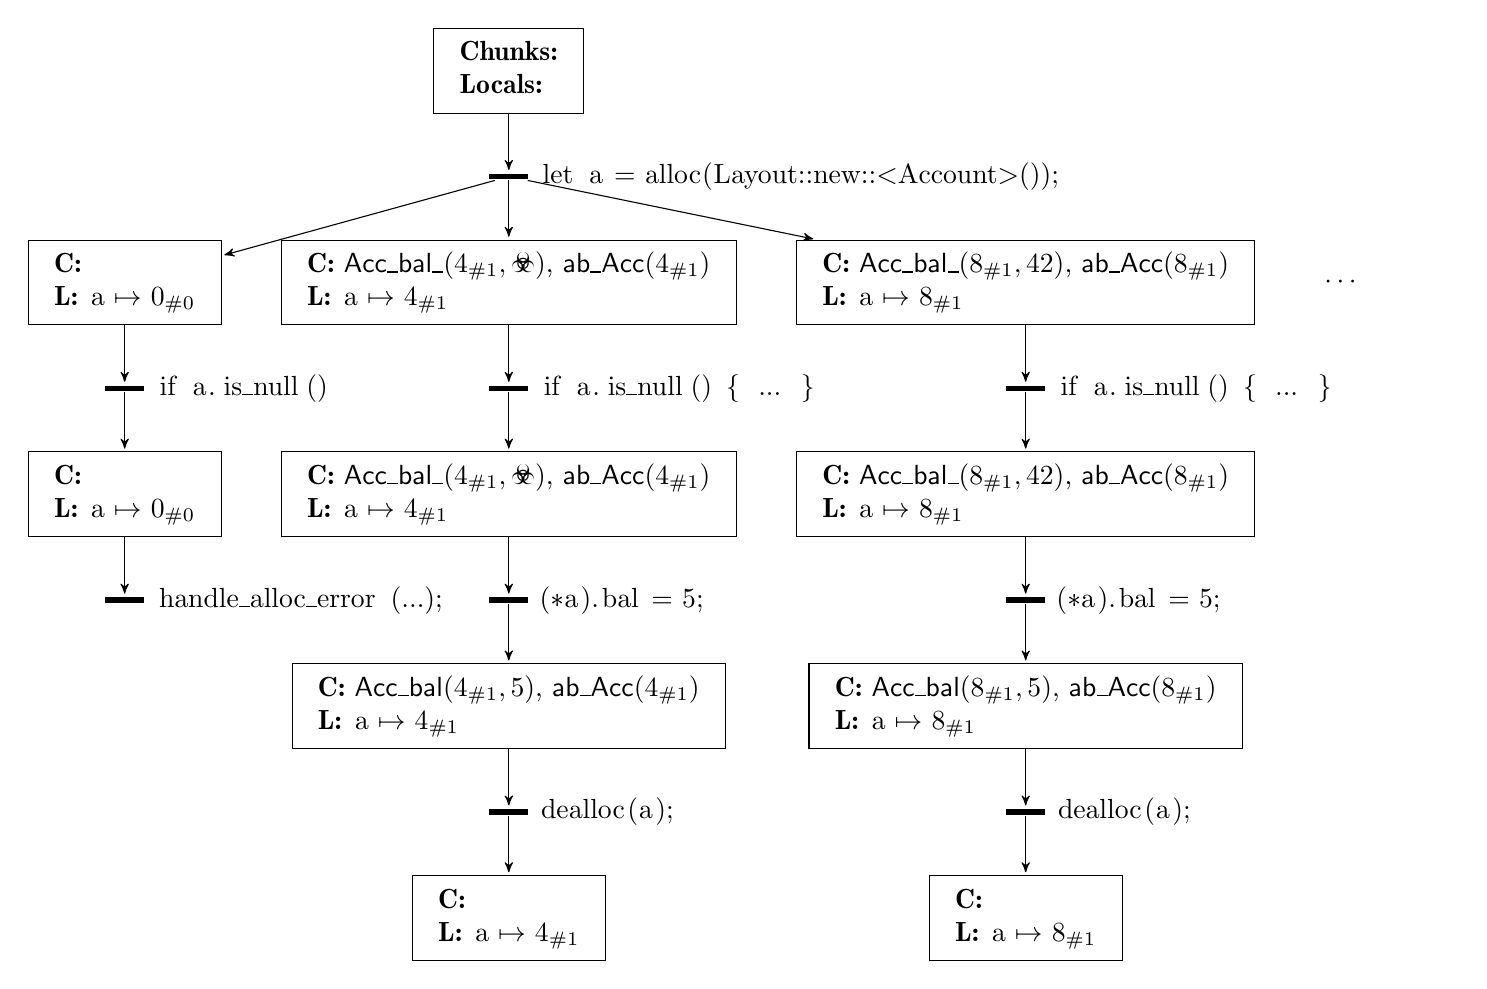
\begin{tikzpicture}
\node [state] (s1) {\begin{tabular}{l l}
\textbf{Chunks:}\\
\textbf{Locals:}\\
\end{tabular}};
\node [transitionV] (t1) [below=of s1, label=right:\parbox{10cm}{\lstinline|let a = alloc(Layout::new::<Account>());|}] {}
  edge [pre] (s1);

\node [state] (s22) [below=of t1] {\begin{tabular}{l @{\ } l}
\textbf{C:} & $\mathsf{Acc\_bal\_}(4_{\#1}, \poison)$, $\mathsf{ab\_Acc}(4_{\#1})$\\
\textbf{L:} & \lstinline|a| $\mapsto$ $4_{\#1}$
\end{tabular}}
  edge [pre] (t1);
\node [state] (s23) [right=of s22] {\begin{tabular}{l @{\ } l}
\textbf{C:} & $\mathsf{Acc\_bal\_}(8_{\#1}, 42)$, $\mathsf{ab\_Acc}(8_{\#1})$\\
\textbf{L:} & \lstinline|a| $\mapsto$ $8_{\#1}$
\end{tabular}}
  edge [pre] (t1);
\node (s24) [right=of s23] {$\cdots$};

\node [state] (s21) [left=of s22] {\begin{tabular}{l @{\ } l}
\textbf{C:}\\
\textbf{L:} & \lstinline|a| $\mapsto$ $0_{\#0}$
\end{tabular}}
  edge [pre] (t1);
\node [transitionV] (t21) [below=of s21, label=right:\parbox{5cm}{\lstinline|if a.is_null()|}] {}
  edge [pre] (s21);
\node [state] (s31) [below=of t21] {\begin{tabular}{l @{\ } l}
\textbf{C:}\\
\textbf{L:} & \lstinline|a| $\mapsto$ $0_{\#0}$
\end{tabular}}
  edge [pre] (t21);
\node [transitionV] (t31) [below=of s31, label=right:\parbox{5cm}{\lstinline|handle_alloc_error(...);|}] {}
  edge [pre] (s31);

\node [transitionV] (t22) [below=of s22, label=right:\parbox{5cm}{\lstinline|if a.is_null() \{ ... \}|}] {}
  edge [pre] (s22);
\node [state] (s32) [below=of t22] {\begin{tabular}{l @{\ } l}
\textbf{C:} & $\mathsf{Acc\_bal\_}(4_{\#1}, \poison)$, $\mathsf{ab\_Acc}(4_{\#1})$\\
\textbf{L:} & \lstinline|a| $\mapsto$ $4_{\#1}$
\end{tabular}}
  edge [pre] (t22);
\node [transitionV] (t32) [below=of s32, label=right:\parbox{5cm}{\lstinline|(*a).bal = 5;|}] {}
  edge [pre] (s32);
\node [state] (s42) [below=of t32] {\begin{tabular}{l @{\ } l}
\textbf{C:} & $\mathsf{Acc\_bal}(4_{\#1}, 5)$, $\mathsf{ab\_Acc}(4_{\#1})$\\
\textbf{L:} & \lstinline|a| $\mapsto$ $4_{\#1}$
\end{tabular}}
  edge [pre] (t32);
\node [transitionV] (t42) [below=of s42, label=right:\parbox{5cm}{\lstinline|dealloc(a);|}] {}
  edge [pre] (s42);
\node [state] (s52) [below=of t42] {\begin{tabular}{l @{\ } l}
\textbf{C:}\\
\textbf{L:} & \lstinline|a| $\mapsto$ $4_{\#1}$
\end{tabular}}
  edge [pre] (t42);

\node [transitionV] (t23) [below=of s23, label=right:\parbox{5cm}{\lstinline|if a.is_null() \{ ... \}|}] {}
  edge [pre] (s23);
\node [state] (s33) [below=of t23] {\begin{tabular}{l @{\ } l}
\textbf{C:} & $\mathsf{Acc\_bal\_}(8_{\#1}, 42)$, $\mathsf{ab\_Acc}(8_{\#1})$\\
\textbf{L:} & \lstinline|a| $\mapsto$ $8_{\#1}$
\end{tabular}}
  edge [pre] (t23);
\node [transitionV] (t33) [below=of s33, label=right:\parbox{5cm}{\lstinline|(*a).bal = 5;|}] {}
  edge [pre] (s33);
\node [state] (s43) [below=of t33] {\begin{tabular}{l @{\ } l}
\textbf{C:} & $\mathsf{Acc\_bal}(8_{\#1}, 5)$, $\mathsf{ab\_Acc}(8_{\#1})$\\
\textbf{L:} & \lstinline|a| $\mapsto$ $8_{\#1}$
\end{tabular}}
  edge [pre] (t33);
\node [transitionV] (t43) [below=of s43, label=right:\parbox{5cm}{\lstinline|dealloc(a);|}] {}
  edge [pre] (s43);
\node [state] (s53) [below=of t43] {\begin{tabular}{l @{\ } l}
\textbf{C:}\\
\textbf{L:} & \lstinline|a| $\mapsto$ $8_{\#1}$
\end{tabular}}
  edge [pre] (t43);
\end{tikzpicture}
\end{center}
\caption{Concrete execution tree of the program of Figure~\ref{figure:illegal-access1} (after uncommenting the \lstinline|if| statement). We abbreviate \textbf{Chunks} as \textbf{C}, \textbf{Locals} as \textbf{L}, \lstinline|Account| as \lstinline|Acc|, \lstinline|balance| as \lstinline|bal|, \lstinline|my_account| as \lstinline|a|, and $\mathsf{alloc\_block}$ as $\mathsf{ab}$. Note that the tree is not shown fully: the \lstinline|alloc| node has one child node for each combination $(\ell, s)$ of a memory location $\ell$ for the new account and an initial state $s$ of its \lstinline|balance| field. Note that in Rust, a pointer/memory location $\ell = a_p$ consists of an \emph{address} $a$ and a \emph{provenance} $p$; see \url{https://www.ralfj.de/blog/2018/07/24/pointers-and-bytes.html}. The null pointer has address 0 and special provenance $\#0$. Pointers to allocated memory blocks have as their provenance the allocation identifier ($\#1$ is the provenance of the first block allocated by the program) and have a nondeterministically selected address; the diagram shows 4 and 8 as examples of such addresses for conciseness. (Note: the provenance model suggested here is just an example; in reality, VeriFast abstracts over the precise provenance model, and in fact, by specifying \lstinline|-assume_no_provenance| on the command line, you can make VeriFast assume (unsoundly!) that all pointers have the same provenance $\#0$.) The initial state $s$ of a memory location can be the poisoned state ($\poison$) or some value, e.g. 42.}\label{fig:concrete-execution-tree}
\end{figure}

The concrete execution tree of the corrected version of the program of Figure~\ref{figure:illegal-access1} is shown in Figure~\ref{fig:concrete-execution-tree}. Notice that it is in fact (practically) infinite-width. For this example program, the concrete execution tree is not infinite-depth, because the program has no loops or recursion. If the program had a loop with an unbounded number of iterations, the tree would have been infinite-depth as well.

\begin{exercise}\label{exercise:symex-tree}
Draw the symbolic execution tree of the \lstinline|main| function of the corrected version of the program of Figure~\ref{figure:illegal-access1}. A symbolic execution tree differs from a concrete execution tree in that each state includes a set of used \emph{symbols} and a set of \emph{assumptions} about these symbols, and in that the heap chunks and the local variable bindings are expressed using these symbols. Furthermore, by using these symbols, a single path in a symbolic execution tree can be used to describe infinitely many corresponding paths in the corresponding concrete execution tree.
\end{exercise}

\section{alloc\_block Chunks}\label{section:malloc_block}

To better understand why the $\mathit{alloc}$ statement
generates both an $\mathsf{Account\_balance\_}$ chunk and an
$\mathsf{alloc\_}$\-$\mathsf{block\_Account}$ chunk, change
the program so that the struct instance is allocated as a local
variable on the stack instead of being allocated on the heap:
\begin{lstlisting}
fn main()
//@ req true;
//@ ens true;
{
    unsafe {
        let mut my_account_local = Account { balance: 0 };
        let my_account = &raw mut my_account_local;
        (*my_account).balance = 5;
        dealloc(my_account as *mut u8, Layout::new::<Account>());
    }
}
\end{lstlisting}
This program first allocates an instance of struct
$\mathsf{Account}$ on the stack and calls it
$\mathsf{my\_account\_local}$. It then assigns the address of this
struct instance to pointer variable $\mathsf{my\_account}$. The
remainder of the program is as before: the program sets
the $\mathsf{balance}$ field to value 5 and then attempts to
deallocate the struct instance.

If we ask VeriFast to verify this program, VeriFast reports the
error $$\textsf{No matching heap chunks:
alloc\_block\_Account(my\_account\_local\_addr)}$$ at the
$\mathit{dealloc}$ statement. Indeed, the call of $\mathit{dealloc}$ is incorrect,
since $\mathit{dealloc}$ may only be applied to a struct instance
allocated on the heap by $\mathsf{alloc}$, not to a struct
instance allocated on the stack as a local variable.

VeriFast detects this error as follows: 1) VeriFast generates an
$\mathsf{alloc\_block}$ chunk only for struct instances
allocated using $\mathit{alloc}$, not for struct instances
allocated on the stack. 2) When verifying a $\mathit{dealloc}$
statement, VeriFast checks that an $\mathsf{alloc\_block}$
chunk exists for the struct instance being freed.

Notice that, in contrast, the $\mathsf{account\_balance\_}$ chunk
is generated in both cases. As a result, the statement that
initializes the $\mathsf{balance}$ field verifies successfully,
regardless of whether the struct instance was allocated on the
heap or on the stack.

\section{Functions and Contracts}\label{section:functions}

We continue to play with the example of the previous section.
The example currently consists of only one function: the main
function. Let's add another function. Write an $\mathsf{Account}$ associated function
$\mathsf{set\_balance}$ that takes a pointer to an
$\mathsf{Account}$ struct instance and a integer amount, and
assigns this amount to the struct instance's $\mathsf{balance}$
field. Then replace the field assignment in the main function
with a call to this function. We now have the following
program:

\begin{lstlisting}
// verifast_options{ignore_unwind_paths}
use std::alloc::{Layout, alloc, handle_alloc_error, dealloc};

struct Account {
    balance: i32
}

impl Account {

    unsafe fn set_balance(my_account: *mut Account, new_balance: i32) {
        (*my_account).balance = new_balance;
    }

}

fn main()
//@ req true;
//@ ens true;
{
    unsafe {
        let my_account = alloc(Layout::new::<Account>()) as *mut Account;
        if my_account.is_null() {
            handle_alloc_error(Layout::new::<Account>());
        }
        Account::set_balance(my_account, 5);
        dealloc(my_account as *mut u8, Layout::new::<Account>());
    }
}
\end{lstlisting}

If we try to verify the new program, VeriFast complains that
the new function has no contract. Indeed, VeriFast verifies
each function separately, so it needs a precondition and a
postcondition for each function to describe the initial and
final state of calls of the function.

Add the same contract that the main function has:
\begin{lstlisting}
unsafe fn set_balance(my_account: *mut Account, new_balance: i32)
//@ req true;
//@ ens true;
\end{lstlisting}
Notice that contracts, like all VeriFast annotations, are in
comments, so that the Rust compiler ignores them. VeriFast also
ignores comments, except the ones that are marked with an at
(\verb|@|) sign.

VeriFast now no longer complains about missing contracts.
However, it now complains that the field assignment in the body
of $\mathsf{Account{::}set\_balance}$ cannot be verified because
the symbolic heap does not contain a heap chunk that grants
permission to access this field. To fix this, we need to
specify in the function's precondition that the function
requires permission to access the $\mathsf{balance}$ field of
the $\mathsf{Account}$ struct instance pointed to by
$\mathsf{my\_account}$. We achieve this simply by mentioning the
heap chunk in the precondition:
\begin{lstlisting}
unsafe fn set_balance(my_account: *mut Account, new_balance: i32)
//@ req Account_balance_(my_account, _);
//@ ens true;
\end{lstlisting}
Notice that we use an underscore in the position where the
state of the field belongs. This indicates that we do not care
about the old state of the field when the function is
called.\footnote{VeriFast also supports a more concise syntax
for field chunks. For example,
\lstinline!Account_balance_(my_account, _)! can also be written as
\lstinline!(*my_account).balance |-> _!.
In fact, the latter (field chunk-specific) syntax is generally recommended
over the former (generic chunk) syntax because it causes
VeriFast to take into account the field chunk-specific information that there is at most one
chunk for a given field, and that the field's value is within the limits of
its type. However, for didactical reasons, in this tutorial we initially use the generic
chunk syntax so that the chunks written in the annotations and the heap chunks shown in the VeriFast IDE look the same.}

VeriFast now highlights the brace that closes the body of the
function. This means we successfully verified the field
assignment. However, VeriFast now complains that the function
leaks heap chunks. For now, let's simply work around this error
message by inserting a $\mathbf{leak}$ command, which indicates
that we're happy to leak this heap chunk. We will come back to
this later.
\begin{lstlisting}
unsafe fn set_balance(my_account: *mut Account, new_balance: i32)
//@ req Account_balance_(my_account, _);
//@ ens true;
{
    (*my_account).balance = new_balance;
    //@ leak Account_balance(my_account, _);
}
\end{lstlisting}

Function $\mathsf{Account::set\_balance}$ now verifies, and
VeriFast attempts to verify function $\mathsf{main}$. It
complains that it cannot deallocate the $\mathsf{Account}$ struct
instance because it does not have permission to access the
$\mathsf{balance}$ field. Indeed, the symbolic heap contains
the $\mathsf{alloc\_block\_Account}$ chunk but not the
$\mathsf{Account\_balance}$ chunk. What happened to it? Let's
find out by stepping through the symbolic execution path.
Select the fourth step. The $\mathsf{alloc}$ statement is about
to be executed and the symbolic heap is empty. Select the next
step. The $\mathsf{alloc}$ statement has added the
$\mathsf{Account\_balance\_}$ chunk and the
$\mathsf{alloc\_block\_Account}$ chunk.

The if statement has no effect.

We then arrive at the call of $\mathsf{Account{::}set\_balance}$.
You will notice that this execution step has two sub-steps,
labeled ``Consuming assertion'' and ``Producing assertion''.
The verification of a function call consists of
\emph{consuming} the function's precondition and then
\emph{producing} the function's postcondition. The precondition
and the postcondition are \emph{assertions}, i.e., expressions
that may include heap chunks in addition to ordinary logic.
Consuming the precondition means passing the heap chunks
required by the function to the function, thus removing them
from the symbolic heap. Producing the postcondition means
receiving the heap chunks offered by the function when it
returns, thus adding them to the symbolic heap.

\begin{figure}
\begin{center}
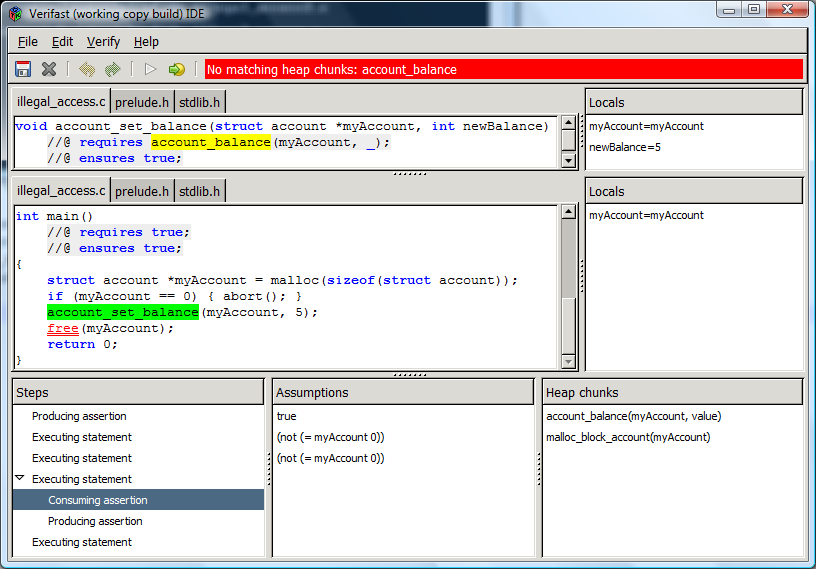
\includegraphics[width=10cm]{illegal_access3.png}
\end{center}
\caption{When stepping through a function call, VeriFast shows both the call site (in green, in the lower pane) and the callee's contract (in yellow, in the upper pane).}\label{figure:call}
\end{figure}

Selecting the ``Consuming assertion'' step changes the layout
of the VeriFast window (see Figure~\ref{figure:call}).
The source code pane is split into two
parts. The upper part is used to display the contract of the
function being called, while the lower part is used to display
the function being verified. (Since in this example the
function being called is so close to the function being
verified, it is likely to be shown in the lower part as well.)
The call being verified is shown on a green background. The
part of the contract being consumed or produced is shown on a
yellow background. If you move from the ``Consuming assertion''
step to the ``Producing assertion'' step, you notice that the
``Consuming assertion'' step removes the
$\mathsf{Account\_balance\_}$ chunk from the symbolic heap.
Conceptually, it is now in use by the
$\mathsf{Account{::}set\_balance}$ function while the
$\mathsf{main}$ function waits for this function to return.
Since function $\mathsf{Account{::}set\_balance}$'s postcondition
does not mention any heap chunks, the ``Producing assertion''
step does not add anything to the symbolic heap.

It is now clear why VeriFast complained that
$\mathsf{Account{::}set\_balance}$ leaked heap chunks: since the
function did not return the $\mathsf{Account\_balance}$ chunk
to its caller, the chunk was lost and the field could never be
accessed again. VeriFast considers this an error since it is
usually not the intention of the programmer; furthermore, if
too many memory locations are leaked, the program will run out
of memory.

It is now also clear how to fix the error: we must specify in
the postcondition of function $\mathsf{Account{::}set\_balance}$
that the function must hand back the
$\mathsf{Account\_balance}$ chunk to its caller.
\begin{lstlisting}
unsafe fn set_balance(my_account: *mut Account, new_balance: i32)
//@ req Account_balance_(my_account, _);
//@ ens Account_balance(my_account, new_balance);
{
    (*my_account).balance = new_balance;
}
\end{lstlisting}
 This
eliminates the leak error message and the error at the
$\mathit{dealloc}$ statement. The program now verifies. Notice
that we refer to the $\mathsf{new_balance}$ parameter in the
position where the value of the field belongs; this means that
the value of the field when the function returns must be equal
to the value of the parameter.

\begin{exercise}\label{exercise:account}
Now factor out the creation and the disposal of the
$\mathsf{Account}$ struct instance into separate functions as
well. The creation function should initialize the balance to
zero. Note: if you need to mention multiple heap chunks in an
assertion, separate them using the \emph{separating conjunction}
\lstinline!&*&! (ampersand-star-ampersand). Also, you can refer
to a function's return value in its postcondition by the name
\lstinline!result!.
\end{exercise}

\section{Patterns}

Now, let's add a function that returns the current balance, and
let's test it in the main function. Here's our first attempt:

\begin{lstlisting}
impl Account { 

    unsafe fn get_balance(my_account: *mut Account) -> i32
    //@ req Account_balance(my_account, _);
    //@ ens Account_balance(my_account, _);
    {
        (*my_account).balance
    }    

}

fn main()
//@ req true;
//@ ens true;
{
    unsafe {
        let my_account = Account::create();
        Account::set_balance(my_account, 5);
        let b = Account::get_balance(my_account);
        std::hint::assert_unchecked(b == 5);
        Account::dispose(my_account);
    }
}
\end{lstlisting}

The new function verifies successfully, but VeriFast complains
that it cannot prove the condition \lstinline!b == 5!. When
VeriFast is asked to check a condition, it first translates the
condition to a logical formula, by replacing each variable by
its symbolic value. We can see in the symbolic store, displayed
in the Locals pane, that the symbolic value of variable
\lstinline|b| is the logical symbol $\mathsf{b}$. Therefore, the
resulting logical formula is $\mathsf{b} = 5$. VeriFast then
attempts to derive this formula from the \emph{path condition},
i.e., the formulae shown in the Assumptions pane. Since the
only assumption in this case is $\mathsf{true}$, VeriFast
cannot prove the condition.

The problem is that the postcondition of function
$\mathsf{Account{::}get\_balance}$ does not specify the
function's return value. It does not state that the return
value is equal to the value of the $\mathsf{balance}$ field
when the function is called. To fix this, we need to be able to
assign a name to the value of the balance field when the
function is called. We can do so by replacing the underscore in
the precondition by the \emph{pattern} \lstinline!?theBalance!.
This causes the name \lstinline!theBalance! to be bound to the
value of the $\mathsf{balance}$ field. We can then use this
name in the postcondition to specify the return value using an
equality condition. A function's return value is available in
the function's postcondition under the name \lstinline!result!.
Logical conditions and heap chunks in an assertion must be
separated using the separating conjunction \lstinline!&*&!.
\begin{lstlisting}
unsafe fn get_balance(my_account: *mut Account) -> i32
//@ req Account_balance(my_account, ?theBalance);
//@ ens Account_balance(my_account, theBalance) &*& result == theBalance;
{
    (*my_account).balance
}    
\end{lstlisting}
Notice that we use the \lstinline!theBalance! name also to
specify that the function does not modify the value of the
$\mathsf{balance}$ field, by using the name again in the field
value position in the postcondition.

The program now verifies. Indeed, if we use the \textbf{Run to
cursor} command to run to the $\mathit{assert}$ statement, we
see that the assumption \lstinline!b = 5! has appeared in the
Assumptions pane. If we step up, we see that it was added when
the equality condition in function
$\mathsf{Account{::}get\_balance}$'s postcondition was produced.
If we step up further, we see that the variable
\lstinline!theBalance! was added to the upper Locals pane when
the field chunk assertion was consumed, and bound to value 5.
It was bound to value 5 because that was the value found in the
symbolic heap. When verifying a function call, the upper Locals
pane is used to evaluate the contract of the function being
called. It initially contains the bindings of the function's
parameters to the arguments specified in the call; additional
bindings appear as patterns are encountered in the contract.
The assumption \lstinline!b = 5! is the logical formula
obtained by evaluating the equality condition %
\lstinline!result == theBalance! under the symbolic store shown
in the upper Locals pane.

\begin{exercise}\label{exercise:deposit}
Add a function that deposits a given amount into an account.
Verify the following \lstinline!main! function.
\begin{lstlisting}[basicstyle=\ttfamily\upshape]
fn main()
//@ req true;
//@ ens true;
{
    unsafe {
        let my_account = Account::create();
        Account::set_balance(my_account, 5);
        Account::deposit(my_account, 10);
        let b = Account::get_balance(my_account);
        std::hint::assert_unchecked(b == 15);
        Account::dispose(my_account);
    }
}
\end{lstlisting}
Note: VeriFast checks for arithmetic overflow. For now, disable
this check in the \textbf{Verify} menu.
\end{exercise}

\begin{exercise}\label{exercise:limit}
Add a field \lstinline!limit! to struct \lstinline!Account! that specifies the minimum balance of the account. (It is typically either zero or a negative number.)
The limit is specified at creation time. Further add a function
to withdraw a given amount from an account. The function must
respect the limit; if withdrawing the requested amount would violate the limit, then the largest amount that can be withdrawn without violating the limit is withdrawn. The function
returns the amount actually withdrawn as its return value. You
will need to use conditional expressions
\lstinline!if condition { value1 } else { value2 }!. Remove function
\lstinline!Account::set_balance!. Use the shorthand notation for
field chunks: \lstinline!(*my_account).balance |-> value!. Verify
the following \lstinline!main! function.
\begin{lstlisting}[basicstyle=\ttfamily\upshape]
fn main()
//@ req true;
//@ ens true;
{
    unsafe {
        let my_account = Account::create(-100);
        Account::deposit(my_account, 200);
        let w1 = Account::withdraw(my_account, 50);
        std::hint::assert_unchecked(w1 == 50);
        let b1 = Account::get_balance(my_account);
        std::hint::assert_unchecked(b1 == 150);
        let w2 = Account::withdraw(my_account, 300);
        std::hint::assert_unchecked(w2 == 250);
        let b2 = Account::get_balance(my_account);
        std::hint::assert_unchecked(b2 == -100);
        Account::dispose(my_account);
    }
}
\end{lstlisting}
\end{exercise}

\section{Predicates}

We continue with the program obtained in
Exercise~\ref{exercise:limit}. We observe that the contracts
are becoming rather long. Furthermore, if we consider the
account ``class'' and the main function to be in different
modules, then the internal implementation details of the
account module are exposed to the main function. We can achieve
more concise contracts as well as information hiding by
introducing a \emph{predicate} to describe an
$\mathsf{account}$ struct instance in the function contracts.
\begin{lstlisting}
/*@
pred Account_pred(my_account: *mut Account, theLimit: i32, theBalance: i32) =
    (*my_account).limit |-> theLimit &*& (*my_account).balance |-> theBalance &*&
    alloc_block_Account(my_account);
@*/
\end{lstlisting}
A predicate is a named, parameterized assertion. Furthermore, it introduces a new type of heap chunk.
An \lstinline!Account_pred! heap chunk bundles an \lstinline!Account_limit! heap chunk, an \lstinline!Account_balance! heap chunk,
and an \lstinline!alloc_block_Account! heap chunk into one.

Let's use this predicate to rewrite the contract of the deposit function. Here's a first attempt:
\begin{lstlisting}
unsafe fn deposit(my_account: *mut Account, amount: i32)
//@ req Account_pred(my_account, ?limit, ?balance) &*& 0 <= amount;
//@ ens Account_pred(my_account, limit, balance + amount);
{
    (*my_account).balance += amount;
}
\end{lstlisting}
This function does not verify. The update of the
\lstinline!balance! field cannot be verified since there is no
\lstinline!Account_balance! heap chunk in the symbolic heap.
There is only an \lstinline!Account_pred! heap chunk. The
\lstinline!Account_pred! heap chunk encapsulates the
\lstinline!Account_balance! heap chunk, but VeriFast does not
``un-bundle'' the \lstinline!Account_pred! predicate
automatically. We must instruct VeriFast to un-bundle predicate
heap chunks by inserting an \lstinline!open! ghost statement:
\begin{lstlisting}
unsafe fn deposit(my_account: *mut Account, amount: i32)
//@ req Account_pred(my_account, ?limit, ?balance) &*& 0 <= amount;
//@ ens Account_pred(my_account, limit, balance + amount);
{
    //@ open Account_pred(my_account, limit, balance);
    (*my_account).balance += amount;
}
\end{lstlisting}
The assignment now verifies, but now VeriFast is stuck at the
postcondition. It complains that it cannot find the
\lstinline!Account_pred! heap chunk that it is supposed to hand
back to the function's caller. The \lstinline!Account_pred!
chunk's constituent chunks are present in the symbolic heap,
but VeriFast does not automatically bundle them up into an
\lstinline!Account_pred! chunk. We must instruct VeriFast to do
so using a \lstinline!close! ghost statement:
\begin{lstlisting}
unsafe fn deposit(my_account: *mut Account, amount: i32)
//@ req Account_pred(my_account, ?limit, ?balance) &*& 0 <= amount;
//@ ens Account_pred(my_account, limit, balance + amount);
{
    //@ open Account_pred(my_account, limit, balance);
    (*my_account).balance += amount;
    //@ close Account_pred(my_account, limit, balance + amount);
}
\end{lstlisting}
The function now verifies. However, the main function does not,
since the call of \lstinline!Account::deposit! expects an
\lstinline!Account_pred! heap chunk.

\begin{exercise}\label{exercise:pred}
Rewrite the remaining contracts using the
\lstinline!Account_pred! predicate. Insert \lstinline!open! and
\lstinline!close! statements as necessary.
\end{exercise}

\section{Recursive Predicates}

In the previous section, we introduced predicates for the sake
of conciseness and information hiding. However, there is an
even more compelling need for predicates: they are the only way
you can describe unbounded-size data structures in VeriFast.
Indeed, in the absence of predicates, the number of memory
locations described by an assertion is linear in the length of
the assertion. This limitation can be overcome through the use
of recursive predicates, i.e., predicates that invoke
themselves.

\begin{exercise}\label{exercise:stack}
Implement a stack of integers using a singly linked list data
structure: implement \lstinline|Stack| associated functions \lstinline!create!,
\lstinline!push!, \lstinline!pop!, and
\lstinline!dispose!. In order to be able to specify the
precondition of \lstinline!pop!, your predicate will need
to have a parameter that specifies the number of elements in
the stack. Function \lstinline!dispose! may be called
only on an empty stack. Do not attempt to specify the contents
of the stack; this is not possible with the annotation elements
we have seen. You will need to use conditional assertions:
\lstinline!if condition { assertion1 } else { assertion2 }!. Note: VeriFast
does not allow the use of field dereferences in
\lstinline!open! statements. If you want to use the value of a
field in an \lstinline!open! statement, you must first store
the value in a local variable. Verify the following main
function:
\end{exercise}
\begin{lstlisting}
fn main()
//@ req true;
//@ ens true;
{
    unsafe {
        let s = Stack::create();
        Stack::push(s, 10);
        Stack::push(s, 20);
        Stack::pop(s);
        Stack::pop(s);
        Stack::dispose(s);
    }
}
\end{lstlisting}

Now, let's extend the solution to Exercise~\ref{exercise:stack}
on page~\pageref{solution:stack} with a
\lstinline!Stack::is_empty! function. Recall the predicate
definitions:
\begin{lstlisting}
pred Nodes(node: *mut Node, count: i32) =
    if node == 0 {
        count == 0
    } else {
        0 < count &*&
        (*node).next |-> ?next &*& (*node).value |-> ?value &*&
        alloc_block_Node(node) &*& Nodes(next, count - 1)
    };

pred Stack(stack: *mut Stack, count: i32) =
    (*stack).head |-> ?head &*& alloc_block_Stack(stack) &*& 0 <= count &*& Nodes(head, count);
\end{lstlisting}

Here's a first stab at a \lstinline!Stack::is_empty! function:
\begin{lstlisting}
unsafe fn is_empty(stack: *mut Stack) -> bool
//@ req Stack(stack, ?count);
//@ ens Stack(stack, count) &*& result == (count == 0);
{
    //@ open Stack(stack, count);
    let result = (*stack).head.is_null();
    //@ close Stack(stack, count);
    result
}
\end{lstlisting}
The function does not verify. VeriFast complains that it cannot
prove the condition \lstinline!result == (count == 0)! in the
postcondition. Indeed, if we look at the assumptions in the
Assumptions pane, they are insufficient to prove this
condition. The problem is that the relationship between the
value of the head pointer and the number of nodes is hidden
inside the \lstinline!Nodes! predicate. We need to open the
predicate, so that the information is added to the assumptions.
Of course, we then need to close it again so that we can close
the \lstinline!Stack! predicate.
\begin{lstlisting}
unsafe fn is_empty(stack: *mut Stack) -> bool
//@ req Stack(stack, ?count);
//@ ens Stack(stack, count) &*& result == (count == 0);
{
    //@ open Stack(stack, count);
    let head = (*stack).head;
    //@ open Nodes(head, count);
    let result = head.is_null();
    //@ close Nodes(head, count);
    //@ close Stack(stack, count);
    result
}
\end{lstlisting}
The function now verifies. What happens exactly is the
following. When VeriFast executes the open statement, it
produces the conditional assertion in the body of the
\lstinline!Nodes! predicate. This causes it to perform a
\emph{case split}. This means that the rest of the function is
verified twice: once under the assumption that the condition is
true, and once under the assumption that the condition is
false. In other words, the execution path splits into two
execution paths, or two \emph{branches}. On both branches, the
postcondition can now be proved easily: on the first branch, we
get the assumptions $\mathsf{head} = \mathsf{null\_pointer}$ and %
$\mathsf{count} = 0$, and on the second branch we get
$\mathsf{head} \neq \mathsf{null\_pointer}$ and $0 < \mathsf{count}$.

\begin{exercise}\label{exercise:dispose}
Modify function \lstinline!Stack::dispose! so that it works even
if the stack still contains some elements. Use a recursive
helper function.\footnote{Warning: VeriFast does not verify
termination; it does not complain about infinite recursion or
infinite loops. That is still your own responsibility.}
\end{exercise}

Notice that VeriFast performs a case split when verifying an
\lstinline!if! statement.

\begin{exercise}\label{exercise:sum}
Add a function \lstinline!Stack::get_sum! that returns the sum
of the values of the elements on the stack. Use a recursive
helper function. The contract need not specify the return value
(since we did not see how to do that yet).
\end{exercise}

\section{Loops}\label{section:loops}

In Exercise~\ref{exercise:dispose}, we implemented
\lstinline!Stack::dispose! using a recursive function. However,
this is not an optimal implementation. If our data structure
contains very many elements, we may create too many activation
records and overflow the call stack. It is more optimal to
implement the function using a loop. Here's a first attempt:\footnote{A \lstinline|while| loop would perhaps be more natural here. Unfortunately, however, VeriFast for Rust supports only \lstinline|loop| loops for now.}
\begin{lstlisting}
unsafe fn dispose(stack: *mut Stack)
//@ req Stack(stack, _);
//@ ens true;
{
    //@ open Stack(stack, _);
    let mut n = (*stack).head;
    loop {
        //@ open Nodes(n, _);
        if n.is_null() {
            break;
        }
        let next = (*n).next;
        dealloc(n as *mut u8, Layout::new::<Node>());
        n = next;
    }
    dealloc(stack as *mut u8, Layout::new::<Stack>());
}
\end{lstlisting}
This function does not verify. VeriFast complains at the loop
because the loop does not specify a loop invariant. VeriFast
needs a loop invariant so that it can verify an arbitrary
sequence of loop iterations by verifying the loop body once,
starting from a symbolic state that represents the start of an
arbitrary loop iteration (not just the first iteration).

Specifically, VeriFast verifies a loop as follows:
\begin{itemize}
\item First, it consumes the loop invariant.
\item Then, it removes the remaining heap chunks from the
    heap (but it remembers them).
\item Then, it assigns a fresh logical symbol to each local
    variable that is modified in the loop body.
\item Then, it produces the loop invariant.
\item Then, it verifies the loop body. If, during verification of the loop body, an execution path \lstinline|break|s out of the loop, at that point the heap chunks that were removed from the symbolic heap when the loop was entered are added back and symbolic execution continues after the loop.
\item Then, it consumes the loop invariant.
\item And then finally it checks for leaks.
        After this step this execution path is
        finished.
\end{itemize}
Notice that this means that the loop can access only those heap
chunks that are mentioned in the loop invariant.

The correct loop invariant for the above function is as
follows:
\begin{lstlisting}
unsafe fn dispose(stack: *mut Stack)
//@ req Stack(stack, _);
//@ ens true;
{
    //@ open Stack(stack, _);
    let mut n = (*stack).head;
    loop {
        //@ inv Nodes(n, _);
        //@ open Nodes(n, _);
        if n.is_null() {
            break;
        }
        let next = (*n).next;
        dealloc(n as *mut u8, Layout::new::<Node>());
        n = next;
    }
    dealloc(stack as *mut u8, Layout::new::<Stack>());
}
\end{lstlisting}

You can inspect the execution of the loop
by commenting out the first \lstinline|dealloc| statement. This will cause
the leak check at the end of the symbolic execution of the loop to fail. Find the
step where the loop invariant is consumed for the first time.
Notice that after this step, the value
of variable \lstinline!n! changes from \lstinline!head0! to
\lstinline!n!, and all chunks are removed from the symbolic
heap.

\begin{exercise}\label{exercise:popn}
Specify and implement function \lstinline!Stack::popn!, which
pops a given number of elements from the stack (and does not
return a result). You may call \lstinline!Stack::pop!
internally. Use a \lstinline!loop! loop. Notice that your loop
invariant must not only enable verification of the loop body,
but must also maintain the relationship between the current
state and the initial state, sufficiently to prove the
postcondition. This often means that you should not overwrite
the function parameter values, since you typically need the
original values in the loop invariant.
\end{exercise}

\section{Inductive Datatypes}\label{section:datatypes}

Let's return to our initial annotated stack implementation (the
solution to Exercise~\ref{exercise:stack}). The annotations do
not specify full functional correctness. In particular, the
contract of function \lstinline!Stack::pop! does not specify the
function's return value. As a result, using these annotations,
we cannot verify the following main function:
\begin{lstlisting}
fn main()
//@ req true;
//@ ens true;
{
    unsafe {
        let s = Stack::create();
        Stack::push(s, 10);
        Stack::push(s, 20);
        let result1 = Stack::pop(s);
        //@ assert result1 == 20;
        let result2 = Stack::pop(s);
        //@ assert result2 == 10;
        Stack::dispose(s);
    }
}
\end{lstlisting}

In order to verify this main function, instead of tracking just
the number of elements in the stack, we need to track the
values of the elements as well. In other words, we need to
track the precise sequence of elements currently stored by the
stack. We can represent a sequence of integers using an
\emph{inductive datatype} \lstinline!i32s!:
\begin{lstlisting}
inductive i32s = i32s_nil | i32s_cons(i32, i32s);
\end{lstlisting}
This declaration declares a type \lstinline!i32s! with two
\emph{constructors} \lstinline!i32s_nil! and
\lstinline!i32s_cons!. \lstinline!i32s_nil! represents the
empty sequence. \lstinline!i32s_cons! constructs a nonempty
sequence given the \emph{head} (the first element) and the
\emph{tail} (the remaining elements). For example, the sequence
1,2,3 can be written as
\begin{lstlisting}
i32s_cons(1, i32s_cons(2, i32s_cons(3, i32s_nil)))
\end{lstlisting}

\begin{exercise}\label{exercise:values}
Replace the \lstinline!count! parameter of the
\lstinline!Nodes! and \lstinline!Stack! predicates with a
\lstinline!values! parameter of type \lstinline!i32s! and
update the predicate bodies. Further update the functions
\lstinline!Stack::create!, \lstinline!Stack::push!, and
\lstinline!Stack::dispose!. Don't worry about \lstinline!Stack::pop! for now.
\end{exercise}

\section{Fixpoint Functions}

How should we update the annotations for function
\lstinline!Stack::pop!? We need to refer to the tail of the
current sequence in the postcondition and in the close
statement. Furthermore, in order to specify the return value,
we need to refer to the head of the current sequence. We can do
so using \emph{fixpoint functions}:
\begin{lstlisting}
fix i32s_head(values: i32s) -> i32 {
    match values {
        i32s_nil => 0,
        i32s_cons(value, values0) => value,
    }
}

fix i32s_tail(values: i32s) -> i32s {
    match values {
        i32s_nil => i32s_nil,
        i32s_cons(value, values0) => values0,
    }
}
\end{lstlisting}
Notice that we can use match expressions on inductive
datatypes. There must be exactly one case for each constructor.
In a case for a constructor that takes parameters, the
specified parameter names are bound to the corresponding
constructor argument values that were used when the value was
constructed. The body of a fixpoint function must be a match
expression on one of the function's parameters (called the
\emph{inductive parameter}). Furthermore, the body of each case
must be an expression (not a block).

In contrast to regular Rust functions, a fixpoint function may be
used in any place where an expression is expected in an
annotation. This means we can use the \lstinline!i32s_head! and
\lstinline!i32s_tail! functions to adapt function
\lstinline!Stack::pop! to the new predicate definitions, and to
specify the return value.

\begin{exercise}\label{exercise:fixpoints}
Do so.
\end{exercise}

We have now specified full functional correctness of our stack
implementation, and VeriFast can now verify the new main
function.

\begin{exercise}\label{exercise:sum_full}
Add a Rust function \lstinline!Stack::get_sum! that returns the sum
of the elements of a given stack. Implement it using a
recursive helper function \lstinline!get_nodes_sum!. Specify
the new Rust functions using a recursive fixpoint function
\lstinline!i32s_sum!. Remember to turn off arithmetic
overflow checking in the \textbf{Verify} menu. Verify the
following main function:
\end{exercise}
\begin{lstlisting}
fn main()
//@ req true;
//@ ens true;
{
    unsafe {
        let s = Stack::create();
        Stack::push(s, 10);
        Stack::push(s, 20);
        let sum = Stack::get_sum(s);
        //@ assert sum == 30;
        let result1 = Stack::pop(s);
        //@ assert result1 == 20;
        let result2 = Stack::pop(s);
        //@ assert result2 == 10;
        Stack::dispose(s);
    }
}
\end{lstlisting}

VeriFast supports recursive fixpoint functions. It enforces
that they always terminate by allowing only direct recursion
and by requiring that the value of the inductive parameter of a
recursive call is a constructor argument of the value of the
inductive parameter of the caller.

\section{Lemmas}\label{section:lemmas}

\emph{Note: Sections~\ref{section:arrays} to
\ref{section:strings} offer an alternative introduction to
recursive predicates. If you are not yet comfortable with
recursive predicates, refer to these sections before starting
the present section.}

Let's return to our initial annotated stack implementation (the
solution to Exercise~\ref{exercise:stack}). Let's add a
\lstinline!Stack::get_count! function that returns the number of
elements in the stack, implemented using a loop:
\begin{lstlisting}
unsafe fn get_count(stack: *mut Stack) -> i32
//@ req Stack(stack, ?count);
//@ ens Stack(stack, count) &*& result == count;
{
    //@ open Stack(stack, count);
    let head = (*stack).head;
    let mut n = head;
    let mut i = 0;
    loop {
        //@ inv true;
        if n.is_null() {
            break;
        }
        n = (*n).next;
        i += 1;
    }
    //@ close Stack(stack, count);
    i
}
\end{lstlisting}
Clearly, the loop invariant \lstinline!true! will not do. What
should it be? We need to express that \lstinline!n! is
somewhere inside our sequence of nodes. One way to do this is
by working with \emph{linked list segments} (or \emph{list
segments} for short). We state in the loop invariant that there
is a list segment from \lstinline!head! to \lstinline!n! and a
separate list segment from \lstinline!n! to 0:
\begin{lstlisting}
//@ inv lseg(head, n, i) &*& lseg(n, 0, count - i);
\end{lstlisting}
We can define the \lstinline!lseg! predicate as follows:
\begin{lstlisting}
pred lseg(first: *mut Node, last: *mut Node, count: i32) =
    if first == last {
        count == 0
    } else {
        0 < count &*& first != 0 &*&
        (*first).value |-> ?value &*& (*first).next |-> ?next &*& alloc_block_Node(first) &*&
        lseg(next, last, count - 1)
    };
\end{lstlisting}
We are not done yet. We need to establish the loop invariant
when first entering the loop. That is, we need to establish
\begin{lstlisting}
lseg(head, head, 0) &*& lseg(head, 0, count)
\end{lstlisting}
The first conjunct is easy: it is empty, so we can just close
it. The second conjunct requires that we rewrite the
\lstinline!Nodes(head, count)! chunk into an equivalent
\lstinline!lseg(head, 0, count)! chunk. Notice that we cannot
do so using a statically bounded number of open and close
operations. We need to use either a loop or a recursive
function. Since VeriFast does not allow loops inside
annotations, we will use a recursive function. We will not use
a regular Rust function, since the function has no purpose at run
time; furthermore, we cannot use a fixpoint function, since the
latter cannot include open or close statements. VeriFast
supports a third kind of function, called \emph{lemma
functions}. They are just like regular Rust functions, except that
they may not perform field assignments or call regular
functions, and they must always terminate. It follows that
calling them has no effect at run time. Their only purpose is
to transform some heap chunks into an equivalent set of heap
chunks, i.e. different heap chunks that represent the same
actual memory values. In contrast with fixpoint functions, they
may be called only through separate call statements, not from
within expressions.

VeriFast checks termination of a lemma function by allowing
only direct recursion and by checking each recursive call as
follows: first, if, after consuming the precondition of the
recursive call, a field chunk is left in the symbolic heap,
then the call is allowed. This is induction on heap size.
Otherwise, if the body of the lemma function is a match
statement on a parameter whose type is an inductive datatype,
then the argument for this parameter in the recursive call must
be a constructor argument of the caller's argument for the same
parameter. This is induction on an inductive parameter.
Finally, if the body of the lemma function is not such a match
statement, then the first heap chunk consumed by the
precondition of the callee must have been obtained from the
first heap chunk consumed by the precondition of the caller
through one or more open operations. This is induction on the
derivation of the first conjunct of the precondition.

We can transform a \lstinline!Nodes! chunk into an
\lstinline!lseg! chunk using the following lemma function:
\begin{lstlisting}
lem Nodes_to_lseg_lemma(first: *mut Node)
    req Nodes(first, ?count);
    ens lseg(first, 0, count);
{
    open Nodes(first, count);
    if first != 0 {
        Nodes_to_lseg_lemma((*first).next);
    }
    close lseg(first, 0, count);
}
\end{lstlisting}
Notice that this lemma is accepted since it performs induction
on heap size.

\begin{exercise}\label{exercise:lemma}
We will need the inverse operation as well. Write a lemma
function \lstinline!lseg_to_Nodes_lemma! that takes an
\lstinline!lseg! chunk that ends in a null pointer and transforms it into a
\lstinline!Nodes! chunk.
\end{exercise}

The \lstinline!Stack::get_count! function now looks as follows:
\begin{lstlisting}
unsafe fn get_count(stack: *mut Stack) -> i32
//@ req Stack(stack, ?count);
//@ ens Stack(stack, count) &*& result == count;
{
    //@ open Stack(stack, count);
    let head = (*stack).head;
    //@ Nodes_to_lseg_lemma(head);
    let mut n = head;
    let mut i = 0;
    //@ close lseg(head, head, 0);
    loop {
        //@ inv lseg(head, n, i) &*& lseg(n, 0, count - i);
        if n.is_null() {
            break;
        }
        //@ open lseg(n, 0, count - i);
        n = (*n).next;
        i += 1;
        // Error!
    }
    //@ open lseg(0, 0, _);
    //@ lseg_to_Nodes_lemma(head);
    //@ close Stack(stack, count);
    i
}
\end{lstlisting}
We are almost done. All that is left to do is to fix the error
that we get at the end of the loop body. At that point, we have
the following chunks:
\begin{lstlisting}
lseg(head, ?old_n, i - 1) &*& (*old_n).value |-> ?value &*& (*old_n).next |-> n &*&
alloc_block_Node(old_n) &*& lseg(n, 0, count - i)
\end{lstlisting}
We need to transform these into the following:
\begin{lstlisting}
lseg(head, n, i) &*& lseg(n, 0, count - i)
\end{lstlisting}
That is, we need to append the node at the old value of
\lstinline!n! to the end of the list segment that starts at
\lstinline!head!. We will again need to use a lemma function
for this. Here's a first attempt:
\begin{lstlisting}
lem lseg_add_lemma(first: *mut Node)
    req
        lseg(first, ?last, ?count) &*& last != 0 &*& (*last).value |-> ?value &*&
        (*last).next |-> ?next &*& alloc_block_Node(last);
    ens lseg(first, next, count + 1);
{
    open lseg(first, last, count);
    if first == last {
        close lseg(next, next, 0);
    } else {
        lseg_add_lemma((*first).next);
    }
    close lseg(first, next, count + 1);
}
\end{lstlisting}
VeriFast complains while trying to perform the final close
operation, on the path where \lstinline!first! equals
\lstinline!last!. It has assumed that \lstinline!first! equals
\lstinline!next! and it cannot prove that \lstinline!count + 1!
equals zero. In our scenario, \lstinline!first! never equals
\lstinline!next!, since \lstinline!first! always points to a
node of the stack, and \lstinline!next! either points to a
separate node or equals 0. However, the precondition of our
lemma function does not express this. In order to include this
information, we need to require the list segment from
\lstinline!next! to 0 as well. By opening and closing this list
segment before we perform the final close operation, we obtain
the information that \lstinline!first! and \lstinline!next! are
distinct. Specifically, whenever VeriFast produces a field
chunk, and another field chunk for the same field is already in
the symbolic heap, it adds an assumption stating that the field
chunks belong to distinct struct instances.

We obtain the following \lstinline!lseg_add_lemma! and
\lstinline!Stack::get_count! functions:
\begin{lstlisting}
/*@
lem lseg_add_lemma(first: *mut Node)
    req lseg(first, ?last, ?count) &*& last != 0 &*& (*last).value |-> ?last_value &*&
        (*last).next |-> ?next &*& alloc_block_Node(last) &*& lseg(next, 0, ?count0);
    ens lseg(first, next, count + 1) &*& lseg(next, 0, count0);
{
    open lseg(first, last, count);
    if first == last {
        close lseg(next, next, 0);
    } else {
        lseg_add_lemma((*first).next);
    }
    open lseg(next, 0, count0);
    close lseg(next, 0, count0);
    close lseg(first, next, count + 1);
}
@*/

impl Stack {
    unsafe fn get_count(stack: *mut Stack) -> i32
    //@ req Stack(stack, ?count);
    //@ ens Stack(stack, count) &*& result == count;
    {
        //@ open Stack(stack, count);
        let head = (*stack).head;
        //@ Nodes_to_lseg_lemma(head);
        let mut n = head;
        let mut i = 0;
        //@ close lseg(head, head, 0);
        loop {
            //@ inv lseg(head, n, i) &*& lseg(n, 0, count - i);
            if n.is_null() {
                break;
            }
            //@ open lseg(n, 0, count - i);
            n = (*n).next;
            i += 1;
            //@ lseg_add_lemma(head);
        }
        //@ open lseg(0, 0, _);
        //@ lseg_to_Nodes_lemma(head);
        //@ close Stack(stack, count);
        i
    }
}
\end{lstlisting}
These now verify.

\begin{exercise}\label{exercise:push_all}
Verify the following function. You'll need an extra lemma.
\end{exercise}
\begin{lstlisting}
unsafe fn push_all(stack: *mut Stack, other: *mut Stack)
//@ req Stack(stack, ?count) &*& Stack(other, ?count0);
//@ ens Stack(stack, count0 + count);
{
    let head0 = (*other).head;
    dealloc(other as *mut u8, Layout::new::<Stack>());
    let mut n = head0;
    if !n.is_null() {
        loop {
            if (*n).next.is_null() {
                break;
            }
            n = (*n).next;
        }
        (*n).next = (*stack).head;
        (*stack).head = head0;
    }
}
\end{lstlisting}

\begin{exercise}\label{exercise:reverse}
Implement, specify, and verify a function
\lstinline!Stack::reverse! that performs in-place reversal of a
stack, i.e., without any memory allocation. Verify full
functional correctness (see Section~\ref{section:datatypes}).
You'll need to define additional fixpoints and lemmas.
\end{exercise}

\section{Function Pointers}\label{section:function-pointers}

Let's write a function that takes a stack and removes those elements that do not satisfy a given predicate:
\begin{lstlisting}
type I32Predicate = unsafe fn(i32) -> bool;

unsafe fn filter_nodes(n: *mut Node, p: I32Predicate) -> *mut Node
//@ req Nodes(n, _);
//@ ens Nodes(result, _);
{
    if n.is_null() {
        return std::ptr::null_mut();
    } else {
        //@ open Nodes(n, _);
        let keep = p((*n).value);
        let next;
        if keep {
            next = filter_nodes((*n).next, p);
            //@ open Nodes(next, ?count);
            //@ close Nodes(next, count);
            (*n).next = next;
            //@ close Nodes(n, count + 1);
            return n;
        } else {
            next = (*n).next;
            dealloc(n as *mut u8, Layout::new::<Node>());
            let result = filter_nodes(next, p);
            return result;
        }
    }
}

impl Stack {
    unsafe fn filter(stack: *mut Stack, p: I32Predicate)
    //@ req Stack(stack, _);
    //@ ens Stack(stack, _);
    {
        //@ open Stack(stack, _);
        let head = filter_nodes((*stack).head, p);
        //@ assert Nodes(head, ?count);
        (*stack).head = head;
        //@ open Nodes(head, count);
        //@ close Nodes(head, count);
        //@ close Stack(stack, count);
    }
}

unsafe fn neq_20(x: i32) -> bool
//@ req true;
//@ ens true;
{
    x != 20
}

fn main() {
    unsafe {
        let s = Stack::create();
        Stack::push(s, 10);
        Stack::push(s, 20);
        Stack::filter(s, neq_20);
        Stack::dispose(s);
    }
}
\end{lstlisting}

This program does not verify. VeriFast does not know what
contract to use to verify the call of \lstinline!p! in function
\lstinline!filter_nodes!. Specifically, when symbolically executing a call of a function pointer \lstinline|p|,
VeriFast looks for a \emph{function type chunk} \lstinline|is_T(p)| in the symbolic heap that asserts that \lstinline|p| satisfies \emph{VeriFast function type \lstinline|T|}.

We therefore need to define a VeriFast function type:
\begin{lstlisting}
/*@
fn_type I32Predicate() = unsafe fn(x: i32) -> bool;
    req true;
    ens true;
@*/
\end{lstlisting}
It is like a Rust type definition, except that it also associates a precondition and a postcondition
with the type.

We must update the precondition of functions \lstinline|filter_nodes| and \lstinline|Stack::filter| to
assert an appropriate function type chunk:
\begin{lstlisting}
unsafe fn filter_nodes(n: *mut Node, p: I32Predicate) -> *mut Node
//@ req Nodes(n, _) &*& [_]is_I32Predicate(p);
//@ ens Nodes(result, _);

impl Stack {
    unsafe fn filter(stack: *mut Stack, p: I32Predicate)
    //@ req Stack(stack, _) &*& [_]is_I32Predicate(p);
    //@ ens Stack(stack, _);
\end{lstlisting}
(The \lstinline|[_]| prefix denotes duplicability of the chunk; it will be explained in Section~\ref{section:leaking}.)

Finally, before calling \lstinline|Stack::filter| in the main function, we must \emph{produce} the function type chunk, using a \lstinline|produce_fn_ptr_chunk T(f)()(params) { proof }| ghost command. This command requires a sequence of ghost commands \lstinline|proof|, exactly one of which must be a \lstinline|call();| statement, that proves that the function \lstinline|f| satisfies the function type's contract. Specifically, VeriFast checks the proof by first producing the function type's precondition, then symbolically executing \lstinline|proof|, where \lstinline|call();| is symbolically executed like a call of \lstinline|f|, and finally consumes the function type's postcondition:
\begin{lstlisting}
fn main()
//@ req true;
//@ ens true;
{
    unsafe {
        let s = Stack::create();
        Stack::push(s, 10);
        Stack::push(s, 20);
        /*@
        produce_fn_ptr_chunk I32Predicate(neq_20)()(x) {
            call();
        }
        @*/
        Stack::filter(s, neq_20);
        Stack::dispose(s);
    }
}
\end{lstlisting}

\begin{exercise}\label{exercise:filter}
Put all the pieces together.
\end{exercise}

The state of our \lstinline!Stack::filter! function is
unsatisfactory in two ways: firstly, the
\lstinline!I32Predicate! function cannot read any memory
locations, since its precondition does not require any heap
chunks; it follows that you cannot filter all elements that are
greater than some user-provided value, for example. This will
be solved using parameterized function types in
Section~\ref{section:predicate-families}. Secondly, the
implementation re-assigns each next pointer, even if only a few
elements are removed. This will be solved using by-reference
parameters in Section~\ref{section:byref-params}.

\section{By-Reference Parameters}\label{section:byref-params}

Here's an alternative implementation of the
\lstinline!Stack::filter! function from
Section~\ref{section:function-pointers}. Instead of
re-assigning each next pointer, it passes a pointer to the next
pointer and only re-assigns it when it changes.
\begin{lstlisting}
unsafe fn filter_nodes(n: *mut *mut Node, p: I32Predicate) {
    if !(*n).is_null() {
        let keep = p((**n).value);
        if keep {
            filter_nodes(&raw mut (**n).next, p);
        } else {
            let next_ = (**n).next;
            dealloc(*n as *mut u8, Layout::new::<Node>());
            *n = next_;
            filter_nodes(n, p);
        }
    }
}

impl Stack {
    unsafe fn filter(stack: *mut Stack, p: I32Predicate) {
        filter_nodes(&raw mut (*stack).head, p);
    }
}
\end{lstlisting}
In this program, we are effectively passing the pointer to the
current node to function \lstinline!filter_nodes! by reference.
Inside function \lstinline!filter_nodes!, we dereference
\lstinline!n! to obtain the pointer to the current node.
VeriFast treats pointer dereferences in a way similar to field
dereferences. However, instead of looking in the symbolic heap
for a field chunk, it looks for a generic \lstinline|points_to| chunk. Predicate \lstinline!points_to! is
defined in \texttt{prelude\_core.rsspec} as follows:
\begin{lstlisting}
pred points_to<T>(p: *T; v: T);
\end{lstlisting}
(We will discuss the meaning of the semicolon later; for now,
just read it like a comma.) Like in the case of a field chunk,
the first argument is the address of the variable, and the
second argument is the current value of the variable.

It follows that the following is a valid contract for function
\lstinline!filter_nodes!:
\begin{lstlisting}
unsafe fn filter_nodes(n: *mut *mut Node, p: I32Predicate)
//@ req points_to(n, ?node) &*& Nodes(node, _) &*& [_]is_I32Predicate(p);
//@ ens points_to(n, ?node0) &*& Nodes(node0, _);
\end{lstlisting}

In order to be able to call \lstinline!filter_nodes! from
\lstinline!Stack::filter!, we must produce a \lstinline!points_to!
chunk. Specifically, we must transform the
\lstinline!Stack_head! chunk into a \lstinline!points_to! chunk.
We do this simply by opening the \lstinline!Stack_head! chunk.
To turn the pointer chunk back into a \lstinline!Stack_head!
chunk, we simply close the \lstinline!Stack_head! chunk again:
\begin{lstlisting}
unsafe fn filter(stack: *mut Stack, p: I32Predicate)
//@ req Stack(stack, _) &*& [_]is_I32Predicate(p);
//@ ens Stack(stack, _);
{
    //@ open Stack(stack, _);
    //@ open Stack_head(stack, _);
    filter_nodes(&raw mut (*stack).head, p);
    //@ close Stack_head(stack, ?head);
    //@ open Nodes(head, ?count);
    //@ close Nodes(head, count);
    //@ close Stack(stack, count);
}
\end{lstlisting}

\begin{exercise}\label{exercise:byref}
Verify function \lstinline!filter_nodes!.
\end{exercise}

Note: in the same way that field chunk assertions can be written more elegantly using a points-to syntax, generic \lstinline|points_to| chunk assertions can be written using a points-to syntax as well. For example, we can also write the spec of \lstinline!filter_nodes! as follows:
\begin{lstlisting}
unsafe fn filter_nodes(n: *mut *mut Node, p: I32Predicate)
//@ req *n |-> ?node &*& Nodes(node, _) &*& [_]is_I32Predicate(p);
//@ ens *n |-> ?node0 &*& Nodes(node0, _);
\end{lstlisting}

\section{Arithmetic Overflow}

Consider the following program:
\begin{lstlisting}
fn thirty_thousand() -> i16
//@ req true;
//@ ens result == 30000;
{ 30_000 }

fn main()
//@ req true;
//@ ens true;
{
  let a = thirty_thousand();
  let b = thirty_thousand();
  let c: i16 = a + b;
  unsafe { std::hint::assert_unchecked(b < c); }
}
\end{lstlisting}
The addition in function \lstinline|main| performs arithmetic overflow: the mathematical result of the addition is outside the limits of the type. Rust considers arithmetic overflow to be an error: in a debug build, the addition panics. (In a release build, the addition wraps around; in this example, this leads to undefined behavior due to the failure of the subsequent unchecked assert.)

VeriFast, too, reports arithmetic overflow as an error by default. Indeed, it does not accept the example program. Sometimes, however, it is useful to postpone worrying about arithmetic overflows; for that reason, VeriFast offers the option to disable the \emph{Check arithmetic overflow} setting in the Verify menu. Be aware, however, that this may lead to unsoundness: with this setting disabled, VeriFast simply assumes that no arithmetic overflow occurs and accepts the example program, even though it has undefined behavior.

Note that for the Rust types \lstinline|usize| and \lstinline|isize|, the limits depend on the compiler's target architecture. VeriFast assumes the same limits that the Rust compiler uses: when verifying a program on a 64-bit machine, VeriFast assumes that \lstinline|usize| and \lstinline|isize| are 64 bits wide.

Now, consider the following function:
\begin{lstlisting}
unsafe fn i16_add(x: *mut i16, y: *mut i16) -> i16
//@ req points_to(x, ?vx) &*& points_to(y, ?vy);
//@ ens points_to(x, vx) &*& points_to(y, vy) &*& result == vx + vy;
{
    let xv = *x;
    let yv = *y;
    xv + yv
}
\end{lstlisting}
This function performs arithmetic overflow and is rejected by VeriFast. (Note: inside annotations, arithmetic operations are interpreted mathematically, so the expression \verb|vx + vy| in the \verb|ens| clause has the mathematical meaning regardless of the Rust type of this expression; it follows that the values of expressions inside annotations are not necessarily within the limits of their Rust type.)

Let's try to fix this function. Here's a first attempt:
\begin{lstlisting}
unsafe fn i16_add(x: *mut i16, y: *mut i16) -> i16
//@ req points_to(x, ?vx) &*& points_to(y, ?vy);
//@ ens points_to(x, vx) &*& points_to(y, vy) &*& result == vx + vy;
{
    let xv = *x;
    let yv = *y;
    if 0 <= xv {
        if i16::MAX - xv < yv {
            std::process::abort();
        }
    } else {
        if yv < i16::MIN - xv {
            std::process::abort();
        }
    }
    xv + yv
}
\end{lstlisting}
Even though this function is now correct,
VeriFast does not accept it. This is because VeriFast checks
that the results of the arithmetic operations are within the
bounds of the type, but it does not assume that the original
values are within the bounds of the type. These assumptions are
not generated automatically in general. In order to generate these assumptions, we must insert
\lstinline!produce_limits! ghost commands into the code. The
argument of a \lstinline!produce_limits! command must be the
name of a Rust local variable (i.e., not a local variable declared
in an annotation). The following program verifies.
\begin{lstlisting}
unsafe fn i16_add(x: *mut i16, y: *mut i16) -> i16
//@ req points_to(x, ?vx) &*& points_to(y, ?vy);
//@ ens points_to(x, vx) &*& points_to(y, vy) &*& result == vx + vy;
{
    let xv = *x;
    let yv = *y;
    //@ produce_limits(xv);
    //@ produce_limits(yv);
    if 0 <= xv {
        if i16::MAX - xv < yv {
            std::process::abort();
        }
    } else {
        if yv < i16::MIN - xv {
            std::process::abort();
        }
    }
    xv + yv
}
\end{lstlisting}

Note: this is a contrived example; in reality, one should of course use Rust's \lstinline|i16::checked_add| method instead.

Also, the limits of the values of variables \emph{are} produced automatically if the points-to syntax is used to assert the chunks. The following verifies:
\begin{lstlisting}
unsafe fn i16_add(x: *mut i16, y: *mut i16) -> i16
//@ req *x |-> ?vx &*& *y |-> ?vy;
//@ ens *x |-> vx &*& *y |-> vy &*& result == vx + vy;
{
    let xv = *x;
    let yv = *y;
    if 0 <= xv {
        if i16::MAX - xv < yv {
            std::process::abort();
        }
    } else {
        if yv < i16::MIN - xv {
            std::process::abort();
        }
    }
    xv + yv
}
\end{lstlisting}

\section{Parameterized Function Types}\label{section:predicate-families}

Let's go back to the \lstinline!Stack::filter! function from
Section~\ref{section:function-pointers}. Suppose we want to
remove all occurrences of some user-provided value from the
stack:
\begin{lstlisting}
type I32Predicate = unsafe fn(data: *mut u8, i32) -> bool;

unsafe fn filter_nodes(n: *mut Node, p: I32Predicate, data: *mut u8) -> *mut Node {
    if n.is_null() {
        std::ptr::null_mut()
    } else {
        let keep = p(data, (*n).value);
        if keep {
            let next = filter_nodes((*n).next, p, data);
            (*n).next = next;
            n
        } else {
            let next = (*n).next;
            dealloc(n as *mut u8, Layout::new::<Node>());
            let result = filter_nodes(next, p, data);
            result
        }
    }
}

impl Stack {
    unsafe fn filter(stack: *mut Stack, p: I32Predicate, data: *mut u8) {
        let head = filter_nodes((*stack).head, p, data);
        (*stack).head = head;
    }
}

unsafe fn neq_a(data: *mut u8, x: i32) -> bool
{
    let result = x != *(data as *mut i32);
    result
}

unsafe fn read_i32() -> i32
//@ req true;
//@ ens true;
//@ assume_correct
{
    let mut line = String::new();
    std::io::stdin().read_line(&mut line).unwrap();
    line.parse().unwrap()
}

fn main() {
    unsafe {
        let s = Stack::create();
        Stack::push(s, 10);
        Stack::push(s, 20);
        let mut a = read_i32();
        Stack::filter(s, neq_a, &raw mut a as *mut u8);
        Stack::dispose(s);
    }
}
\end{lstlisting}

How do we adapt the proof? Here's an attempt:
\begin{lstlisting}
/*@

pred neq_a_data(data: *mut u8) = *(data as *mut i32) |-> ?_;

fn_type I32Predicate() = unsafe fn(data: *mut u8, x: i32) -> bool;
    req neq_a_data(data);
    ens neq_a_data(data);

@*/

impl Stack {
    unsafe fn filter(stack: *mut Stack, p: I32Predicate, data: *mut u8)
    //@ req Stack(stack, _) &*& [_]is_I32Predicate(p) &*& neq_a_data(data);
    //@ ens Stack(stack, _) &*& neq_a_data(data);
    { ... }
}

unsafe fn neq_a(data: *mut u8, x: i32) -> bool
//@ req neq_a_data(data);
//@ ens neq_a_data(data);
{
    //@ open neq_a_data(data);
    let result = x != *(data as *mut i32);
    //@ close neq_a_data(data);
    result
}

fn main()
//@ req true;
//@ ens true;
{
    unsafe {
        let s = Stack::create();
        Stack::push(s, 10);
        Stack::push(s, 20);
        let mut a = read_i32();
        /*@
        produce_fn_ptr_chunk I32Predicate(neq_a)()(data, x) {
            call();
        }
        @*/
        //@ close neq_a_data(&a as *mut u8);
        Stack::filter(s, neq_a, &raw mut a as *mut u8);
        //@ open neq_a_data(&a as *mut u8);
        Stack::dispose(s);
    }
}
\end{lstlisting}

This proof goes through, but it is not modular: the proof of the stack module depends on the \lstinline|neq_a_data|
predicate which is specific to the particular client program.

The solution is to \emph{parameterize} the \lstinline|I32Predicate| VeriFast function type by the predicate
that describes the data, by declaring a \emph{function type parameter} \lstinline|data_pred| between the first set of parentheses:
\begin{lstlisting}
/*@
fn_type I32Predicate(data_pred: pred(*mut u8)) = unsafe fn(data: *mut u8, x: i32) -> bool;
    req data_pred(data);
    ens data_pred(data);
@*/
\end{lstlisting}
Correspondingly, we need to pass an argument for this function type parameter as an extra argument to the \lstinline|is_I32Predicate| function type chunk:
\begin{lstlisting}
unsafe fn filter_nodes(n: *mut Node, p: I32Predicate, data: *mut u8) -> *mut Node
//@ req Nodes(n, _) &*& [_]is_I32Predicate(p, ?data_pred) &*& data_pred(data);
//@ ens Nodes(result, _) &*& data_pred(data);
{ ... }

impl Stack {
    unsafe fn filter(stack: *mut Stack, p: I32Predicate, data: *mut u8)
    //@ req Stack(stack, _) &*& [_]is_I32Predicate(p, ?data_pred) &*& data_pred(data);
    //@ ens Stack(stack, _) &*& data_pred(data);
    { ... }
}
\end{lstlisting}
And we need to specify an argument for each of a VeriFast function type's parameters between the second set of parentheses of the \lstinline|produce_fn_ptr_chunk| ghost command:
\begin{lstlisting}
fn main()
//@ req true;
//@ ens true;
{
    unsafe {
        let s = Stack::create();
        Stack::push(s, 10);
        Stack::push(s, 20);
        let mut a = read_i32();
        /*@
        produce_fn_ptr_chunk I32Predicate(neq_a)(neq_a_data)(data, x) {
            call();
        }
        @*/
        //@ close neq_a_data(&a as *mut u8);
        Stack::filter(s, neq_a, &raw mut a as *mut u8);
        //@ open neq_a_data(&a as *mut u8);
        Stack::dispose(s);
    }
}
\end{lstlisting}

\begin{exercise}\label{exercise:map}
Add a function \lstinline!Stack::map! that takes a function $f$
that takes an \lstinline|i32| and returns an \lstinline|i32|. \lstinline!Stack::map!
replaces the value of each element of the stack with the result
of applying $f$ to it.

Write a client program that creates a stack containing the
values 10, 20, 30; then reads a value from the user; and then
adds this value to each element of the stack using
\lstinline!Stack::map!. Verify the memory safety of the
resulting program.
\end{exercise}

\section{Generics}\label{section:generics}

Consider the solution to Exercise~\ref{exercise:reverse}, where
we verified full functional correctness of a
\lstinline!stack_reverse! function for a stack of integers. We
used an \lstinline!ints! inductive datatype, fixpoint functions
\lstinline!append! and \lstinline!reverse!, and lemmas
\lstinline!append_nil! and \lstinline!append_assoc!. Suppose,
now, that we need the same functionality for a stack of
pointers. Clearly, since C does not support generics, we will
need to copy-paste the C code and replace \lstinline!int! with
\lstinline!void *! throughout. However, fortunately, VeriFast
does support generics for inductive datatypes, fixpoint
functions, lemmas, and predicates, so instead of copy-pasting
all of these, we can parameterize them by the element type.
Here are parameterized versions of \lstinline!ints!,
\lstinline!append!, and \lstinline!append_nil!:
\begin{lstlisting}
inductive list<t> = nil | cons(t, list<t>);

fixpoint list<t> append<t>(list<t> xs, list<t> ys) {
    switch (xs) {
        case nil: return ys;
        case cons(x, xs0): return cons<t>(x, append<t>(xs0, ys));
    }
}

lemma void append_nil<t>(list<t> xs)
    requires true;
    ensures append<t>(xs, nil<t>) == xs;
{
    switch (xs) {
        case nil:
        case cons(x, xs0):
            append_nil<t>(xs0);
    }
}
\end{lstlisting}
As you can see, an inductive datatype definition, fixpoint
function definition, or lemma definition accepts an optional
\emph{type parameter list}, which is a list of \emph{type
parameters} enclosed in angle brackets. Inside the definition,
the type parameters can be used just like other types. Whenever
a type-parameterized datatype, fixpoint, lemma, predicate, or
constructor of a type-parameterized datatype, is mentioned, a
\emph{type argument list} has to be supplied, which is a list
of types enclosed in angle brackets.

Here's what predicates \lstinline!nodes! and \lstinline!stack!
and function \lstinline!stack_reverse! look like for stacks of
pointers:
\begin{lstlisting}
predicate nodes(struct node *node, list<void *> values) =
    node == 0 ?
        values == nil<void *>
    :
        node->next |-> ?next &*& node->value |-> ?value &*& malloc_block_node(node) &*&
        nodes(next, ?values0) &*& values == cons<void *>(value, values0);

predicate stack(struct stack *stack, list<void *> values) =
    stack->head |-> ?head &*& malloc_block_stack(stack) &*& nodes(head, values);

void stack_reverse(struct stack *stack)
    //@ requires stack(stack, ?values);
    //@ ensures stack(stack, reverse<void *>(values));
{
    //@ open stack(stack, values);
    struct node *n = stack->head;
    struct node *m = 0;
    //@ close nodes(m, nil<void *>);
    //@ append_nil<void *>(reverse<void *>(values));
    while (n != 0)
        /*@
        invariant
            nodes(m, ?values1) &*& nodes(n, ?values2) &*&
            reverse<void *>(values) == append<void *>(reverse<void *>(values2), values1);
        @*/
    {
        //@ open nodes(n, values2);
        struct node *next = n->next;
        //@ assert nodes(next, ?values2tail) &*& n->value |-> ?value;
        n->next = m;
        m = n;
        n = next;
        //@ close nodes(m, cons<void *>(value, values1));
        //@ append_assoc<void *>(reverse<void *>(values2tail), cons<void *>(value, nil<void *>), values1);
    }
    //@ open nodes(n, _);
    stack->head = m;
    //@ close stack(stack, reverse<void *>(values));
}
\end{lstlisting}

Thanks to generics, we can now re-use the same datatypes,
fixpoints, and lemmas for both stacks of ints and stacks of
pointers. However, this approach does seem to introduce a lot
of syntactic overhead, considering how we need to insert type
argument lists everywhere. Fortunately, VeriFast performs
\emph{type argument inference}. If VeriFast encounters an
occurrence of a type-parameterized entity in an expression and
no type argument list was specified, VeriFast will infer the
type argument list. Since VeriFast's type system has no
subtyping, a simple unification-based inference approach is
sufficient. The result is that you almost never have to supply
type argument lists in expressions explicitly. Specifically, in
the example, all type argument lists in expressions can be
omitted. Note: VeriFast does not infer type argument lists in
types; that is, when you mention a type-parameterized inductive
datatype, you must always supply the type arguments explicitly.

Of course, the \lstinline!list! datatype is useful much more
generally than just for stacks of integers and stacks of
pointers. In fact, verification of any non-trivial program will
require the use of lists. For this reason, VeriFast comes with
a header file \verb|list.h| that includes the list datatype,
all of the fixpoints and lemmas used in the example, and many
more. This header file is implicitly included in each file that
is verified by VeriFast, so you do not need to include it
explicitly. Note: This also means that you cannot define your
own versions of \lstinline!nil!, \lstinline!cons!, or other
elements provided by \verb|list.h|, since this would result in
a name clash.

\section{Predicate Values}\label{section:predvals}

In the previous section, we obtained a stack of pointers. In
this section, we will use this stack to keep track of a
collection of objects.

Let's try to verify the following program. It is a stack-based
calculator for 2D vectors. It uses the stack from the previous
section. The user can push a vector onto the stack, replace the
top two vectors with their sum, and pop the top vector to print
it.

\begin{lstlisting}
struct vector {
    int x;
    int y;
};

struct vector *create_vector(int x, int y)
{
    struct vector *result = malloc(sizeof(struct vector));
    if (result == 0) abort();
    result->x = x;
    result->y = y;
    return result;
}

int main()
{
    struct stack *s = create_stack();
    while (true)
    {
        char c = input_char();
        if (c == 'p') {
            int x = input_int();
            int y = input_int();
            struct vector *v = create_vector(x, y);
            stack_push(s, v);
        } else if (c == '+') {
            bool empty = stack_is_empty(s);
            if (empty) abort();
            struct vector *v1 = stack_pop(s);
            empty = stack_is_empty(s);
            if (empty) abort();
            struct vector *v2 = stack_pop(s);
            struct vector *sum = create_vector(v1->x + v2->x, v1->y + v2->y);
            free(v1);
            free(v2);
            stack_push(s, sum);
        } else if (c == '=') {
            bool empty = stack_is_empty(s);
            if (empty) abort();
            struct vector *v = stack_pop(s);
            output_int(v->x);
            output_int(v->y);
            free(v);
        } else {
            abort();
        }
    }
}
\end{lstlisting}

The specification of \lstinline!create_vector! is easy:

\begin{lstlisting}
//@ predicate vector(struct vector *v) = v->x |-> _ &*& v->y |-> _ &*& malloc_block_vector(v);

struct vector *create_vector(int x, int y)
    //@ requires true;
    //@ ensures vector(result);
\end{lstlisting}

The tricky part is the loop invariant for the loop in
\lstinline!main!. The loop invariant should state that we have
a stack at \lstinline!s!, and furthermore, that for each
element of \lstinline!s!, we have a vector. We can express the
first part using the assertion \lstinline!stack(s, ?values)!,
and we can easily write a recursive predicate to express the
second part:

\begin{lstlisting}
predicate vectors(list<struct vector *> vs) =
    switch (vs) {
        case nil: return true;
        case cons(v, vs0): return vector(v) &*& vectors(vs0);
    };
\end{lstlisting}

This would work fine. However, it is unfortunate that we have
to define a new predicate whenever we wish to express that we
have a given predicate for each element of a list. To address
this, VeriFast supports \emph{predicate values}. That is, you
can pass a predicate as an argument to another predicate. This
allows us to generalize the above \lstinline!vectors! predicate
as follows:

\begin{lstlisting}
predicate foreach(list<void *> vs, predicate(void *) p) =
    switch (vs) {
        case nil: return true;
        case cons(v, vs0): return p(v) &*& foreach(vs0, p);
    };
\end{lstlisting}

Using generics, we can even generalize this predicate further,
to work for lists of arbitrary values:

\begin{lstlisting}
predicate foreach<t>(list<t> vs, predicate(t) p) =
    switch (vs) {
        case nil: return true;
        case cons(v, vs0): return p(v) &*& foreach(vs0, p);
    };
\end{lstlisting}

Note that type argument inference allows us to omit the type
argument for the recursive \lstinline!foreach! call.

This predicate is so generally useful that we included it in
\texttt{list.h}; as a result, it is automatically available in
each file and you do not need to define it yourself.

\begin{exercise}\label{exercise:foreach}
Verify the program using \lstinline!foreach!.
\end{exercise}

\section{Predicate Constructors}\label{section:predctors}

Let's add a twist to the program of the previous section:
\begin{lstlisting}
struct vector *create_vector(int limit, int x, int y)
{
    if (x * x + y * y > limit * limit) abort();
    struct vector *result = malloc(sizeof(struct vector));
    if (result == 0) abort();
    result->x = x;
    result->y = y;
    return result;
}

int main()
{
    int limit = input_int();
    struct stack *s = create_stack();
    while (true)
    {
        char c = input_char();
        if (c == 'p') {
            int x = input_int();
            int y = input_int();
            struct vector *v = create_vector(limit, x, y);
            stack_push(s, v);
        } else if (c == '+') {
            bool empty = stack_is_empty(s);
            if (empty) abort();
            struct vector *v1 = stack_pop(s);
            empty = stack_is_empty(s);
            if (empty) abort();
            struct vector *v2 = stack_pop(s);
            struct vector *sum = create_vector(limit, v1->x + v2->x, v1->y + v2->y);
            free(v1);
            free(v2);
            stack_push(s, sum);
        } else if (c == '=') {
            bool empty = stack_is_empty(s);
            if (empty) abort();
            struct vector *v = stack_pop(s);
            int x = v->x;
            int y = v->y;
            free(v);
            assert(x * x + y * y <= limit * limit);
            output_int(x);
            output_int(y);
        } else {
            abort();
        }
    }
}
\end{lstlisting}
The program now starts by asking the user for a number that
will serve as a limit on the size of the vectors. When creating
a vector, the program checks that its size does not exceed the
limit; otherwise it aborts. When printing a vector, the program
asserts that the vector satisfies the size limit.

How do we verify this assert statement?

We will need to extend the \lstinline!vector! predicate to
include the information that the vector's size is within the
limit. However, the limit is a local variable and is not in
scope in the predicate definition. So we need to pass it as an
additional argument. But then we can no longer use the
\lstinline!foreach! predicate, since it expects a predicate
that takes just one parameter. To address this, VeriFies
supports \emph{partially applied predicates}, in the form of
\emph{predicate constructors}. To verify the example program,
we can define a predicate constructor \lstinline!vector! as
follows:
\begin{lstlisting}
/*@
predicate_ctor vector(int limit)(struct vector *v) =
    v->x |-> ?x &*& v->y |-> ?y &*& malloc_block_vector(v) &*& x * x + y * y <= limit * limit;
@*/
\end{lstlisting}
We can express that for each element of a list
\lstinline!values! we have a vector that satisfies limit
\lstinline!limit! as follows:
\begin{lstlisting}
foreach(values, vector(limit))
\end{lstlisting}
That is, wherever we can use a predicate name, we can also use
a predicate constructor applied to an argument list. We can do
so in open statements, in close statements, and in assertions.

Note: VeriFast currently does not support patterns in predicate
constructor argument positions.

\begin{exercise}\label{exercise:predctors}
Verify the program.
\end{exercise}

\section{Multithreading}\label{section:multithreading}

Consider the following program that walks a binary tree of
integers, computes the factorial of the value of each node, sums
up the results, and prints the sum to the console.
\begin{lstlisting}
int rand();

int fac(int x)
{
    int result = 1;
    while (x > 1)
    {
        result = result * x;
        x = x - 1;
    }
    return result;
}

struct tree {
    struct tree *left;
    struct tree *right;
    int value;
};

struct tree *make_tree(int depth)
{
    if (depth == 0) {
        return 0;
    } else {
        struct tree *left = make_tree(depth - 1);
        struct tree *right = make_tree(depth - 1);
        int value = rand();
        struct tree *t = malloc(sizeof(struct tree));
        if (t == 0) abort();
        t->left = left;
        t->right = right;
        t->value = value % 2000;
        return t;
    }
}

int tree_compute_sum_facs(struct tree *tree)
{
    if (tree == 0) {
        return 1;
    } else {
        int leftSum = tree_compute_sum_facs(tree->left);
        int rightSum = tree_compute_sum_facs(tree->right);
        int f = fac(tree->value);
        return leftSum + rightSum + f;
    }
}

int main()
{
    struct tree *tree = make_tree(22);
    int sum = tree_compute_sum_facs(tree);
    printf("%i", sum);
    return 0;
}
\end{lstlisting}

\begin{exercise}\label{exercise:threads0}
Verify the memory safety of this program. You may leak the tree (see Section~\ref{section:functions}) after computing the sum.
\end{exercise}

This program takes 14 seconds on the author's machine. However,
the author's machine is a dual core machine, so we might be
able to get a speedup if we distribute the work amongst two
threads, which may then be scheduled by the operating system on
both cores simultaneously.

Unfortunately, writing multithreaded programs currently requires using platform-specific APIs.\footnote{The 2011 edition of the C programming language standard introduced a standard multithreading library, but it is still not supported on all important platforms.}
However, the VeriFast distribution includes a wrapper around
these APIs that offers a uniform interface across all supported
platforms. It is defined in \texttt{threading.h} and
implemented in \texttt{threading.c}; both files are in the
VeriFast \texttt{bin} directory. VeriFast automatically looks
for header files in its \texttt{bin} directory, so to use these
APIs, simply add the line
\begin{lstlisting}
#include "threading.h"
\end{lstlisting}
to the top of your file. In this section, we will be using the
functions \lstinline!thread_start_joinable! and \lstinline!thread_join!
from \texttt{threading.h}, defined as follows:
\begin{lstlisting}
typedef void thread_run_joinable(void *data);

struct thread;

struct thread *thread_start_joinable(void *run, void *data);

void thread_join(struct thread *thread);
\end{lstlisting}
Function \lstinline!thread_start_joinable! takes a pointer to a
\lstinline!run! function and executes this function in a new
thread. Any data required by the run function can be passed via
the \lstinline!data! parameter of \lstinline!thread_start_joinable!,
which is simply passed through to the \lstinline!run! function.
\lstinline!thread_start_joinable! returns a thread handle, which can be
used to join with the created thread using function
\lstinline!thread_join!. The latter waits until the specified
thread has finished.

We can use these functions to speed up our example program as
follows:
\begin{lstlisting}
struct sum_data {
    struct thread *thread;
    struct tree *tree;
    int sum;
};

void summator(struct sum_data *data)
{
    int sum = tree_compute_sum_facs(data->tree);
    data->sum = sum;
}

struct sum_data *start_sum_thread(struct tree *tree)
{
    struct sum_data *data = malloc(sizeof(struct sum_data));
    struct thread *t = 0;
    if (data == 0) abort();
    data->tree = tree;
    t = thread_start_joinable(summator, data);
    data->thread = t;
    return data;
}

int join_sum_thread(struct sum_data *data)
{
    thread_join(data->thread);
    return data->sum;
}

int main()
{
    struct tree *tree = make_tree(22);
    struct sum_data *leftData = start_sum_thread(tree->left);
    struct sum_data *rightData = start_sum_thread(tree->right);
    int sumLeft = join_sum_thread(leftData);
    int sumRight = join_sum_thread(rightData);
    int f = fac(tree->value);
    printf("%i", sumLeft + sumRight + f);
    return 0;
}
\end{lstlisting}
The main program creates a tree of depth 22. It then starts two
threads. The first thread computes the sum of the factorials of
the values of the left subtree, and the second thread computes
the sum of the factorials of the values of the right subtree.
The main thread then waits for both threads to finish, and
finally sums up the results of both threads with the factorial of
the root node's value. On the author's machine, this program
takes only 7 seconds; a twofold speedup!

Now, let's verify the memory safety of this program. The
verification of this program does not require any new
techniques; we will simply apply the techniques we saw in
Sections~\ref{section:function-pointers} and
\ref{section:predicate-families} on function pointers and
predicate families. That is, we specify a contract for the
\lstinline!thread_run_joinable! function pointer type and we use
predicate families so that each program may concretize this
contract according to its needs. The specification of
\lstinline!thread_start_joinable! and \lstinline!thread_join! in
\texttt{threading.h} is as follows:
\begin{lstlisting}
/*@

predicate_family thread_run_pre(void *thread_run)(void *data, any info);
predicate_family thread_run_post(void *thread_run)(void *data, any info);

@*/

typedef void thread_run_joinable(void *data);
    //@ requires thread_run_pre(this)(data, ?info);
    //@ ensures thread_run_post(this)(data, info);

struct thread;

/*@ predicate thread(struct thread *thread, void *thread_run, void *data, any info); @*/

struct thread *thread_start_joinable(void *run, void *data);
    //@ requires is_thread_run_joinable(run) == true &*& thread_run_pre(run)(data, ?info);
    //@ ensures thread(result, run, data, info);

void thread_join(struct thread *thread);
    //@ requires thread(thread, ?run, ?data, ?info);
    //@ ensures thread_run_post(run)(data, info);
\end{lstlisting}
Function \lstinline!thread_start_joinable! requires that the value of
parameter \lstinline!run! is a function pointer that satisfies
the contract of function pointer type \lstinline!thread_run_joinable!;
furthermore, it requires the resources that are required by the
\lstinline!run! function itself, denoted by the
\lstinline!thread_run_pre(run)! predicate family instance. This
predicate takes the \lstinline!data! pointer as an
argument, so that the precondition may describe the data
structure pointed to by this pointer. The \lstinline!info!
parameter of \lstinline!thread_run_pre! and
\lstinline!thread_run_post! is used in advanced scenarios and
may be ignored for now. Function \lstinline!thread_start_joinable!
returns a \lstinline!thread! predicate that contains all
information required to verify the \lstinline!thread_join!
call. Function \lstinline!thread_join! takes this
\lstinline!thread! predicate and returns the resources provided
by the \lstinline!run! function when it returns, as described
by the \lstinline!thread_run_post(run)! predicate family
instance.

\begin{exercise}\label{exercise:threads}
Verify the memory safety of the program. Don't worry about memory deallocation;
simply leak chunks that you no longer need.
\end{exercise}

\section{Fractional Permissions}\label{section:fractions}

Suppose, now, that we want to adapt the program of the previous
section as follows: instead of computing just the sum of the
factorials, we want to compute both the sum of the factorials and
the product of the factorials. Since our machine has two cores,
we want to have two threads: one that computes the sum of the
factorials of the values of the nodes of the tree, and one that
computes the product of the factorials of the values of the
nodes of the tree.

To achieve this, first we generalize our
\lstinline!tree_compute_sum_facs! function to a
\lstinline!tree_fold! function that takes the function that it
should apply to combine the node values as an argument:

\begin{lstlisting}
typedef int fold_function(int acc, int x);

int tree_fold(struct tree *tree, fold_function *f, int acc)
{
    if (tree == 0) {
        return acc;
    } else {
        acc = tree_fold(tree->left, f, acc);
        acc = tree_fold(tree->right, f, acc);
        acc = f(acc, tree->value);
        return acc;
    }
}
\end{lstlisting}

If the elements of the tree $t$ in postfix order are $e_1, e_2,
e_3, e_4$, then \lstinline!tree_fold!$(t, f, a)$ returns
$$f(f(f(f(a, e_1), e_2), e_3), e_4)$$

Likewise, we generalize our summator thread to a folder thread:

\begin{lstlisting}
struct fold_data {
    struct thread *thread;
    struct tree *tree;
    fold_function *f;
    int acc;
};

void folder(struct fold_data *data)
{
    int acc = tree_fold(data->tree, data->f, data->acc);
    data->acc = acc;
}

struct fold_data *start_fold_thread(struct tree *tree, fold_function *f, int acc)
{
    struct fold_data *data = malloc(sizeof(struct fold_data));
    struct thread *t = 0;
    if (data == 0) abort();
    data->tree = tree;
    data->f = f;
    data->acc = acc;
    t = thread_start_joinable(folder, data);
    data->thread = t;
    return data;
}

int join_fold_thread(struct fold_data *data)
{
    thread_join(data->thread);
    return data->acc;
}
\end{lstlisting}

We can re-implement the program of the previous section using folder threads as follows:
\begin{lstlisting}
int sum_function(int acc, int x)
{
    int f = fac(x);
    return acc + f;
}

int main()
    //@ requires true;
    //@ ensures true;
{
    struct tree *tree = make_tree(22);
    //@ open tree(tree, _);
    struct fold_data *leftData = start_fold_thread(tree->left, sum_function, 0);
    struct fold_data *rightData = start_fold_thread(tree->right, sum_function, 0);
    int sumLeft = join_fold_thread(leftData);
    int sumRight = join_fold_thread(rightData);
    int f = fac(tree->value);
    //@ leak tree->left |-> _ &*& tree->right |-> _ &*& tree->value |-> _ &*& malloc_block_tree(tree);
    printf("%i", sumLeft + sumRight + f);
    return 0;
}
\end{lstlisting}

\begin{exercise}\label{exercise:fractions0}
Verify the memory safety of this program.
\end{exercise}

It is now easy to write the program that computes the sums in
one thread and the products in another, and returns the
difference between the product and the sum:
\begin{lstlisting}
int sum_function(int acc, int x)
{
    int f = fac(x);
    return acc + f;
}

int product_function(int acc, int x)
{
    int f = fac(x);
    return acc * f;
}

int main()
{
    struct tree *tree = make_tree(21);
    struct fold_data *sumData = start_fold_thread(tree, sum_function, 0);
    struct fold_data *productData = start_fold_thread(tree, product_function, 1);
    int sum = join_fold_thread(sumData);
    int product = join_fold_thread(productData);
    printf("%i", product - sum);
    return 0;
}
\end{lstlisting}

However, this program cannot be verified using the techniques
that we have seen. The first \lstinline!start_fold_!\-\lstinline!thread! call
consumes the \lstinline!tree! chunk, and therefore VeriFast
will complain that the second call's precondition is not
satisfied. In the system, as explained, only one thread may own
a particular chunk of memory at any one time. Therefore, if the
sum thread owns the tree, the product thread cannot access it
simultaneously. However, this is in fact safe, so long as both
threads only read and do not modify the tree.

VeriFast supports the read-only sharing of chunks of memory
using \emph{fractional permissions}. Each chunk in the VeriFast
symbolic heap has a \emph{coefficient}, which is a real number
between zero, exclusive, and one, inclusive. The default
coefficient is 1 and is not shown. If a chunk's coefficient is
not 1, it is shown to the left of the chunk enclosed in square
brackets. A chunk with coefficient 1 represents a \emph{full
permission}, that is, a \emph{read-write permission}. A chunk
with a coefficient less than 1 represents a \emph{fractional
permission}, that is, a \emph{read-only permission}.

Since the \lstinline!tree_fold! function does not modify the
tree, it requires only a fraction of the \lstinline!tree!
chunk:
\begin{lstlisting}
int tree_fold(struct tree *tree, fold_function *f, int acc)
    //@ requires [?frac]tree(tree, ?depth) &*& is_fold_function(f) == true;
    //@ ensures [frac]tree(tree, depth);
{
    if (tree == 0) {
        return acc;
    } else {
        //@ open [frac]tree(tree, depth);
        acc = tree_fold(tree->left, f, acc);
        acc = tree_fold(tree->right, f, acc);
        acc = f(acc, tree->value);
        return acc;
        //@ close [frac]tree(tree, depth);
    }
}
\end{lstlisting}
Notice that we use a pattern in the coefficient position, so
that the function may be applied to an arbitrarily small
fraction of the \lstinline!tree! chunk. Notice also that we
mention the fraction in the \lstinline!open! and
\lstinline!close! statements. This is not necessary for the
\lstinline!open! statement, since it will by default open
whatever fraction is present in the symbolic heap, but it is
necessary for the \lstinline!close! statement, since it will by
default attempt to close a chunk with coefficient 1.

\begin{exercise}\label{exercise:fractions}
Verify the memory safety of the program. Adapt function
\lstinline!start_fold_thread! so that it requires only a
\lstinline!1/2! fraction of the tree chunk. Note: decimal
notation is not supported; use fractional notation instead.
\end{exercise}

\section{Precise Predicates}\label{section:precise}

The program of the previous section leaks large amounts of
memory. This is fine, since the leaks occur only just before
the program ends anyway. However, suppose now that this program
was part of a larger, long-running program; in that case it
would be important to eliminate the leaks. Therefore, in this
section, let's attempt to eliminate the \lstinline|leak|
commands from the program of the previous section.

First of all, we need to update the C program so that it
properly deallocates all dynamically allocated memory. We need to introduce a function \lstinline|dispose_tree| and update
functions \lstinline|join_fold_thread| and \lstinline|main|:
\begin{lstlisting}
void dispose_tree(struct tree *tree)
{
    if (tree != 0) {
        dispose_tree(tree->left);
        dispose_tree(tree->right);
        free(tree);
    }
}

int join_fold_thread(struct fold_data *data)
{
    thread_join(data->thread);
    int result = data->acc;
    free(data);
    return result;
}

int main()
{
    struct tree *tree = make_tree(21);
    struct fold_data *sumData = start_fold_thread(tree, sum_function, 0);
    struct fold_data *productData = start_fold_thread(tree, product_function, 1);
    int sum = join_fold_thread(sumData);
    int product = join_fold_thread(productData);
    dispose_tree(tree);
    printf("%i", product - sum);
    return 0;
}
\end{lstlisting}

Updating the annotations is slightly trickier. First, let's do
the easy part: verifying the \lstinline|free| statement in
function \lstinline|join_fold_thread|. It already has almost
all required permissions; only the
\lstinline|malloc_block_fold_data| chunk is missing. This chunk
is leaked in function \lstinline|start_fold_thread|. Removing
that \lstinline|leak| statement and adding the chunk to the
\lstinline|ensures| clause of \lstinline|start_fold_thread| and
the \lstinline|requires| clause of \lstinline|join_fold_thread|
solves that problem; the \lstinline|free| statement now
verifies.

All that is left now is to verify the \lstinline|dispose_tree|
call in function \lstinline|main|. It needs full permission for
the tree, i.e.~it needs a \lstinline|tree(tree, _)| chunk.
Notice that each \lstinline|join_fold_thread| call leaks a
\lstinline|[1/2]tree(tree, _)| chunk. We need to update the
annotations of function \lstinline|join_fold_thread| so that it
returns this chunk to its caller instead of leaking it.
However, we currently have no way to identify the tree in the
contract of \lstinline|join_fold_thread|, and a
\lstinline|[1/2]tree(_, _)| chunk would not help us, since we
would not know in \lstinline|main| that the chunk pertains to
the specific tree that we are disposing.

To solve this problem, notice that the tree is pointed to by
field \lstinline|data->tree| in the pre-state of function
\lstinline|join_fold_thread|. However, we cannot mention this
field in function \lstinline|join_fold_thread|'s precondition
since we have passed full permission for this field to the
folder thread.

The solution is to pass only a fraction of the permission for
field \lstinline|data->tree| to the fold thread, and to retain
the remaining fraction in the main thread. To do so, update the
\lstinline|thread_run_pre| and \lstinline|thread_run_post|
predicate family instances, as well as the contracts of
functions \lstinline|start_fold_thread| and
\lstinline|join_fold_thread|:
\begin{lstlisting}
predicate_family_instance thread_run_pre(folder)(struct fold_data *data, any info) =
    [1/2]data->tree |-> ?tree &*& [1/2]tree(tree, _) &*&
    data->f |-> ?f &*& is_fold_function(f) == true &*& data->acc |-> _;
predicate_family_instance thread_run_post(folder)(struct fold_data *data, any info) =
    [1/2]data->tree |-> ?tree &*& [1/2]tree(tree, _) &*&
    data->f |-> ?f &*& is_fold_function(f) == true &*& data->acc |-> _;

struct fold_data *start_fold_thread(struct tree *tree, fold_function *f, int acc)
    //@ requires [1/2]tree(tree, _) &*& is_fold_function(f) == true;
    /*@
    ensures
        [1/2]result->tree |-> tree &*& result->thread |-> ?t &*&
        thread(t, folder, result, _) &*& malloc_block_fold_data(result);
    @*/
int join_fold_thread(struct fold_data *data)
    /*@
    requires
        [1/2]data->tree |-> ?tree &*& data->thread |-> ?t &*&
        thread(t, folder, data, _) &*& malloc_block_fold_data(data);
    @*/
    //@ ensures [1/2]tree(tree, _);
\end{lstlisting}
We can now specify the \lstinline|[1/2]tree(tree, _)| chunk in
the postcondition of function \lstinline|join_fold_thread|.

Notice that we now have two \lstinline|[1/2]tree(tree, _)|
chunks in function \lstinline|main| at the
\lstinline|dispose_tree| call. We have two half chunks, and we
need one full chunk; why does VeriFast not simply merge the two
halves?

The reason is that merging two fractional chunks into a single
chunk is not always a sound (i.e., safe) thing to do. For
example, the following program verifies:
\begin{lstlisting}
/*@

predicate foo(bool b) = true;

predicate bar(int *x, int *y) = foo(?b) &*& b ? integer(x, _) : integer(y, _);

lemma void merge_bar() // This lemma is false!!
    requires [?f1]bar(?x, ?y) &*& [?f2]bar(x, y);
    ensures [f1 + f2]bar(x, y);
{
    assume(false);
}

@*/

int main()
    //@ requires true;
    //@ ensures true;
{
    int x, y;
    //@ close [1/2]foo(true);
    //@ close [1/2]bar(&x, &y);
    //@ close [1/2]foo(false);
    //@ close [1/2]bar(&x, &y);
    //@ merge_bar();
    //@ open bar(&x, &y);
    //@ assert foo(?b);
    //@ if (b) integer_unique(&x); else integer_unique(&y);
    assert(false);
}
\end{lstlisting}
This program demonstrates that assuming that any two fractions
of a given chunk can be merged into a single chunk, leads to
unsoundness (i.e.~a program that raises an assertion failure at
run time verifies successfully). It uses the following lemma
from \lstinline|prelude.h|:
\begin{lstlisting}
lemma void integer_unique(int *p);
    requires [?f]integer(p, ?v);
    ensures [f]integer(p, v) &*& f <= 1;
\end{lstlisting}

The problem is that the two \lstinline|[1/2]bar(&x, &y)| chunks
do not represent the same memory region: one represents
\lstinline|[1/2]integer(&x, _)| and the other one represents
\lstinline|[1/2]integer(&y, _)|. Combining them yields neither
\lstinline|integer(&x, _)| nor \lstinline|integer(&y, _)|.

However, merging two fractions is sound if both fractions
represent the same memory region. To support this, VeriFast
supports the notion of \emph{precise predicates}: you can
declare a predicate as \emph{precise} by writing a semicolon
instead of a comma between the \emph{input parameters} and the
\emph{output parameters} in the predicate's parameter list. For
such a predicate, VeriFast checks that two chunks with the same
input arguments represent the same memory region and always
have the same output arguments. VeriFast automatically merges
fractions of precise predicates that have the same input
arguments.

For example, predicate \lstinline|integer| itself is a precise
predicate; it is declared in \lstinline|prelude.h| as follows:
\begin{lstlisting}
predicate integer(int *p; int v);
\end{lstlisting}
This declaration specifies that predicate \lstinline|integer|
is precise and has one input parameter \lstinline|p| and one
output parameter \lstinline|v|. When VeriFast detects two
chunks \lstinline|[f1]integer(p1, v1)| and
\lstinline|[f2]integer(p2, v2)| and it can prove that
\lstinline|p1| equals \lstinline|p2|, then it merges the chunks
into a single chunk \lstinline|[f1 + f2]integer(p1, v1)| and it
produces the assumption that \lstinline|v1| equals
\lstinline|v2|.

In conclusion, to verify our example program, we need to
declare predicate \lstinline|tree| as precise:
\begin{lstlisting}
predicate tree(struct tree *t; int depth) =
    t == 0 ?
        depth == 0
    :
        t->left |-> ?l &*& t->right |-> ?r &*& t->value |-> ?v &*& malloc_block_tree(t) &*&
        tree(l, ?childDepth) &*& tree(r, childDepth) &*& depth == childDepth + 1;
\end{lstlisting}
Notice that we rephrased the body of the predicate slightly so
that it is accepted by VeriFast's preciseness analysis. The
program now verifies.

The preciseness analysis checks that the body of the predicate
is precise under the input parameters and fixes the output
parameters. The rules for the various forms of assertions being
precise under a set of fixed variables $X$ are as follows:
\begin{itemize}
\item A predicate assertion is precise under $X$ if the
    predicate is precise and the input arguments are fixed
    by $X$; it fixes any variables that appear as output
    arguments. For example, for assertion %
    \lstinline|p(x + y, z)| to be considered precise,
    \lstinline|p| must be a precise predicate. Furthermore,
    suppose it has one input parameter. Then \lstinline|x|
    and \lstinline|y| must be in $X$, and the assertion
    fixes \lstinline|z|.
\item A fractional assertion is precise under $X$ if the
    coefficient is fixed by $X$ or it is a dummy pattern
    and the body is precise under $X$; it fixes any
    variables fixed by its body.
\item A boolean assertion is always precise under any $X$.
    It does not fix any variables, unless it is an equality
    and the left-hand side is a variable and the right-hand
    side is fixed by $X$; in that case, it fixes the
    variable on the left-hand side.
\item A conditional assertion is precise under $X$ if the
    condition is fixed by $X$ and each branch is precise
    under $X$; the fixed variables are the variables that
    are fixed by all branches.
\item Similarly, a \lstinline|switch| assertion is precise
    under $X$ if its operand is fixed by $X$ and each
    branch is precise under the union of $X$ and the
    constructor arguments; the fixed variables are the
    variables that are fixed by all branches.
\item A separating conjunction is precise under $X$ if its
    first operand is precise under $X$, and its second
    operand is precise under the union of $X$ and the
    variables fixed by the first operand. It fixes the
    variables fixed by either operand.
\end{itemize}
That is, the analysis traverses the assertion from left to
right, tracking the set of fixed variables. Input arguments of
nested predicate assertions and branch conditions must depend
only on variables that are already fixed; variables that appear
as output arguments of nested predicate assertions or on the
left-hand side of equalities whose right-hand side is fixed are
added to the set of fixed variables.

\section{Auto-open/close}\label{section:auto-open-close}

In the preceding section, we introduced VeriFast's support for
precise predicates so that we could merge fractions of the same
chunk. However, declaring a predicate as precise has another
advantage: it enables VeriFast's logic for automatically
opening and closing the predicate. This cuts down on the number
of \lstinline|open| and \lstinline|close| commands that you
need to write explicitly.

Specifically, when VeriFast is consuming a predicate assertion,
and no matching chunk exists in the symbolic heap, but the
predicate is precise and all input arguments are specified in
the assertion, then auto-open or auto-close is attempted.
Auto-close is performed if a chunk that appears in the body of
the predicate is found in the symbolic heap; auto-open is
performed if the desired chunk appears in the body of some
chunk that appears in the symbolic heap.

For example, in the program of the preceding section this
allows us to remove all ghost commands for opening or closing
\lstinline|tree| chunks.

\section{Mutexes}\label{section:mutexes}

Suppose we want to write a program that monitors two sensors
and that prints the total number of pulses detected by both
sensors, once every second. We can wait for a pulse from a
given sensor using the API function \lstinline!wait_for_pulse!.
Since pulses come in at both sensors simultaneously, we need to
wait for pulses from each sensor in a separate thread. Whenever
a pulse comes in at a sensor, the corresponding thread
increments a counter that is shared between the threads. The
main thread prints the value of the counter once every second.

When multiple threads access the same variable concurrently,
such as the counter in this example, then they need to
synchronize their accesses; otherwise, two concurrent accesses
may interfere, causing the result to be different from the
result that would be obtained if the accesses were performed
one after the other. Most programming platforms provide various
synchronization constructs to synchronize threads in various
ways.

Perhaps the most common synchronization construct is the mutual
exclusion lock, also known as a lock or a mutex. At any point,
a mutex is in one of two states: either it is free, or it is
held by some thread. A mutex can never be held by more than one
thread. Mutexes provide two operations: acquire and release.
When a thread attempts to acquire a mutex, there are two cases.
\begin{itemize}
\item if the mutex is free, the attempt succeeds and the
    thread holds the mutex until it releases it.
\item if the mutex is held by some other thread, the thread
    that performed the attempt blocks until the mutex is
    free.
\item if the mutex is already held by the thread that
    attempts to acquire it, then the result depends on
    whether the mutex is re-entrant or non-re-entrant. If
    the mutex is re-entrant, the attempt succeeds and the
    thread still holds the lock. If the mutex is
    non-re-entrant, the attempt fails. This either means
    that the thread blocks forever, or that an error occurs
    and the program is terminated.
\end{itemize}

Currently performing synchronization in C programs requires using platform-specific APIs.\footnote{The 2011 edition of the C programming language standard introduced a standard synchronization library, but it is still not supported on all important platforms.} To
enable a uniform interface across all platforms, VeriFast
includes a module \texttt{threading.c} that offers two
synchronization constructs: mutexes and locks. The only
difference between the two is that mutexes are non-re-entrant
and locks are re-entrant. Since mutexes are easier to use, we
will use those in this example.

Here's the source code of the example program:
\begin{lstlisting}
#include "stdlib.h"
#include "threading.h"

void wait_for_pulse(int source);
void sleep(int millis);
void print_int(int n);

struct counter {
    int count;
    struct mutex *mutex;
};

struct count_pulses_data {
    struct counter *counter;
    int source;
};

void count_pulses(struct count_pulses_data *data) {
    struct counter *counter = data->counter;
    int source = data->source;
    free(data);

    struct mutex *mutex = counter->mutex;

    while (true) {
        wait_for_pulse(source);
        mutex_acquire(mutex);
        counter->count++;
        mutex_release(mutex);
    }
}

void count_pulses_async(struct counter *counter, int source) {
    struct count_pulses_data *data = malloc(sizeof(struct count_pulses_data));
    if (data == 0) abort();
    data->counter = counter;
    data->source = source;
    thread_start(count_pulses, data);
}

int main() {
    struct counter *counter = malloc(sizeof(struct counter));
    if (counter == 0) abort();
    counter->count = 0;
    struct mutex *mutex = create_mutex();
    counter->mutex = mutex;

    count_pulses_async(counter, 1);
    count_pulses_async(counter, 2);

    while (true) {
        sleep(1000);
        mutex_acquire(mutex);
        print_int(counter->count);
        mutex_release(mutex);
    }
}
\end{lstlisting}

For this program we use the threading API function
\lstinline!thread_start! instead of
\lstinline!thread_start_joinable!, since we will not be joining
the thread. The specification of function
\lstinline!thread_start! is analogous to the specification of
function \lstinline!thread_start_joinable! discussed in
Section~\ref{section:multithreading}; it is given in header
file \texttt{threading.h} as follows:
\begin{lstlisting}
//@ predicate_family thread_run_data(void *thread_run)(void *data);

typedef void thread_run(void *data);
    //@ requires thread_run_data(this)(data);
    //@ ensures true;

void thread_start(void *run, void *data);
    //@ requires is_thread_run(run) == true &*& thread_run_data(run)(data);
    //@ ensures true;
\end{lstlisting}

It's easy to make mistakes when programming using mutexes. The
worst problem is if the programmer forgets to acquire the mutex
before accessing the data structure that it protects. The
consequence will be incorrect results, but this may be
difficult to diagnose.

Fortunately, VeriFast can help us catch these tricky bugs.
Remember from the preceding sections that as a result of
VeriFast's checks, each thread can access only the memory
locations that it owns, and no two threads can (fully) own the
same memory location at the same time. This prevents
interference from concurrent accesses. But how, then, can
threads share a mutable variable? The answer is, of course,
using mutexes. When a mutex is created, it takes ownership of a
certain set of memory locations, as specified by its \emph{lock
invariant}. When a thread acquires a mutex, the memory
locations that were owned by the mutex now become owned by the
thread, until the thread releases the mutex, at which point the
memory locations again become the property of the mutex. This
way, by sharing a mutex, threads can indirectly share arbitrary
memory locations in a well-synchronized way.

The mutex functions offered by \texttt{threading.c} are
specified in \texttt{threading.h} as follows:
\begin{lstlisting}
struct mutex;

/*@
predicate mutex(struct mutex *mutex; predicate() p);
predicate mutex_held(struct mutex *mutex, predicate() p, int threadId, real frac);
predicate create_mutex_ghost_arg(predicate() p) = true;
@*/

struct mutex *create_mutex();
    //@ requires create_mutex_ghost_arg(?p) &*& p();
    //@ ensures mutex(result, p);

void mutex_acquire(struct mutex *mutex);
    //@ requires [?f]mutex(mutex, ?p);
    //@ ensures mutex_held(mutex, p, currentThread, f) &*& p();

void mutex_release(struct mutex *mutex);
    //@ requires mutex_held(mutex, ?p, currentThread, ?f) &*& p();
    //@ ensures [f]mutex(mutex, p);

void mutex_dispose(struct mutex *mutex);
    //@ requires mutex(mutex, ?p);
    //@ ensures p();
\end{lstlisting}

When you create a mutex, you need to specify the \emph{lock
invariant} that specifies the memory locations that will be
owned by the mutex. You do so by specifying a \emph{predicate
value} (see Section~\ref{section:predvals}). Since the real
function \lstinline!create_mutex! cannot take the predicate
value as a real argument, it takes it as a ghost argument, in
the form of the argument of the
\lstinline!create_mutex_ghost_arg! predicate, which exists only
for this purpose. That is, before calling
\lstinline!create_mutex!, you need to close a
\lstinline!create_mutex_ghost_arg! chunk, whose argument is the
name of the predicate that specifies the lock invariant for the
new mutex. The \lstinline!create_mutex! call consumes the ghost
argument chunk and the lock invariant chunk itself, and
produces a \lstinline!mutex! chunk that represents the mutex.
This chunk specifies the lock invariant as its second argument.

To allow multiple threads to share a mutex, a mutex chunk can
be split into multiple fractions. Only a fraction of a mutex
chunk is required to acquire the mutex. When the mutex is
acquired, the \lstinline!mutex! chunk fraction is transformed
into a \lstinline!mutex_held! chunk, that specifies not only
the mutex and the lock invariant, but also the thread that
acquired the mutex and the coefficient of the mutex chunk
fraction that was used to acquire the mutex. The
\lstinline!mutex_acquire! call additionally produces the lock
invariant, giving the thread access to the memory locations
that were owned by the mutex.

The \lstinline!mutex_release! call consumes a
\lstinline!mutex_held! chunk for the current thread, as well as
the lock invariant, and produces the original \lstinline!mutex!
chunk that was used to acquire the lock.

If necessary, after a program is done using a mutex, it can
reassemble all mutex chunk fractions and dispose the mutex;
this returns ownership of the lock invariant to the thread that
disposes the mutex.

\begin{exercise}\label{exercise:mutexes}
Verify the example program.
\end{exercise}

\section{Leaking and Dummy Fractions}\label{section:leaking}

We start from the example program of the previous section. In
that program, the number of pulse sources is fixed. Suppose
now that sources are connected and disconnected dynamically.
Initially, there are no sources. Suppose there is an API
function \lstinline!wait_for_source! that waits for a new
source to be connected and returns its identifier. Suppose
further that API function \lstinline!wait_for_pulse! now
returns a boolean. If the result is false, it means a new pulse
was detected; if it is true, it means the source has been
disconnected. The goal remains to count the total number of
pulses detected across all sources, and print it out once a
second. The following program achieves this:
\begin{lstlisting}
#include "stdlib.h"
#include "threading.h"

int wait_for_source();
bool wait_for_pulse(int source); // true means the sensor has been removed.
void sleep(int millis);
void print_int(int n);

struct counter {
    int count;
    struct mutex *mutex;
};

struct count_pulses_data {
    struct counter *counter;
    int source;
};

void count_pulses(struct count_pulses_data *data) {
    struct counter *counter = data->counter;
    int source = data->source;
    free(data);

    struct mutex *mutex = counter->mutex;
    bool done = false;
    while (!done) {
        done = wait_for_pulse(source);
        if (!done) {
            mutex_acquire(mutex);
            counter->count++;
            mutex_release(mutex);
        }
    }
}

void count_pulses_async(struct counter *counter, int source) {
    struct count_pulses_data *data = malloc(sizeof(struct count_pulses_data));
    if (data == 0) abort();
    data->counter = counter;
    data->source = source;
    thread_start(count_pulses, data);
}

void print_count(struct counter *counter) {
    struct mutex *mutex = counter->mutex;
    while (true) {
        sleep(1000);
        mutex_acquire(mutex);
        print_int(counter->count);
        mutex_release(mutex);
    }
}

int main() {
    struct counter *counter = malloc(sizeof(struct counter));
    if (counter == 0) abort();
    counter->count = 0;
    struct mutex *mutex = create_mutex();
    counter->mutex = mutex;

    thread_start(print_count, counter);

    while (true) {
        int source = wait_for_source();
        count_pulses_async(counter, source);
    }
}
\end{lstlisting}
Notice that in the example program of the previous section, the
mutex was shared amongst three threads, whereas now it may at
any time be shared amongst arbitrarily many threads. This has
consequences for verification: whereas in the previous section
we could get away with giving each thread one third of the
mutex chunk, splitting up the fractions in the current example
is more complicated.

Furthermore, there is another problem: when a
\lstinline!count_pulses! thread terminates, it still owns a
fraction of the mutex. VeriFast complains about this as part of
its leak check. Indeed, in general, leaking mutexes can cause
the program to eventually run out of memory. However, in the
case of this program, leaking the one mutex is not a problem.
And since the mutex chunk fractions will be leaked anyway and
will never be reassembled to dispose the mutex, there is not
really any point in carefully keeping track of the coefficients
of the various fractions.

VeriFast has a feature called \emph{dummy fractions} that makes
it easy to deal with chunks that are shared among many threads
and that will never be reassembled. Specifically, applying the
\lstinline!leak! ghost command to a chunk does not remove the
chunk but simply replaces the chunk's coefficient with a
\emph{dummy fraction coefficient symbol}. A chunk whose
coefficient is a dummy fraction coefficient symbol is called a
\emph{dummy fraction}. When VeriFast performs the leak check at
the end of each function, it complains only about chunks that
are not dummy fractions.

Dummy fractions are denoted in assertions using dummy patterns,
as in \lstinline![_]chunk(args)!. When consuming an assertion
with a dummy coefficient, the matching chunk must be a dummy
fraction, or VeriFast reports an error since matching the chunk
would implicitly leak it. When producing an assertion with a
dummy coefficient, the produced chunk is a dummy fraction.

To make it easy to share dummy fractions arbitrarily, when
consuming a dummy fraction assertion, VeriFast automatically
splits the matching chunk in two: one part is consumed, and the
other part remains in the symbolic heap.

\begin{exercise}\label{exercise:leaking}
Verify the example program. Leak the mutex chunk directly after
creating it. Use dummy patterns to denote the mutex chunk
fractions' coefficients in assertions.
\end{exercise}

\section{Character Arrays}\label{section:arrays}

Let's verify a program that reads a fixed number of characters
from standard input and then writes them out twice.
Here's a version that reads 5 characters:
\begin{lstlisting}
char getchar();
void putchar(char c);

int main()
{
    char c1 = getchar();
    char c2 = getchar();
    char c3 = getchar();
    char c4 = getchar();
    char c5 = getchar();
    for (int i = 0; i < 2; i++) {
        putchar(c1);
        putchar(c2);
        putchar(c3);
        putchar(c4);
        putchar(c5);
    }
    return 0;
}
\end{lstlisting}
This program works.\footnote{We simplified the return type of \lstinline!getchar! a little bit; the real function returns an int. But this version should compile and run just fine.}
If we run the program and enter \texttt{Hello}, we get back \texttt{HelloHello}.

However, clearly this approach is not practical for large numbers of characters. One approach that works for large numbers of characters is to use an array of characters. We allocate
the array using the standard C function \lstinline!malloc! and then read and write the characters using a recursive function. For now, we don't worry about freeing the array at the end
of the program. Let's first again do a version that reads 5 characters.
\begin{lstlisting}
char getchar();
void putchar(char c);

char *malloc(int count);

void getchars(char *start, int count) {
    if (count > 0) {
        char c = getchar();
        *start = c;
        getchars(start + 1, count - 1);
    }
}

void putchars(char *start, int count) {
    if (count > 0) {
        char c = *start;
        putchar(c);
        putchars(start + 1, count - 1);
    }
}

int main() {
    char *array = malloc(5);
    getchars(array, 5);
    putchars(array, 5);
    putchars(array, 5);
    return 0;
}
\end{lstlisting}
This program works.\footnote{We ignore \lstinline!malloc! failures for now.} Now let's verify it.

It's always a good approach to simply run VeriFast on the program and see where it complains. If you verify the above program, VeriFast complains that the functions have no contract.
Let's start by giving each function the simplest possible contract:
\begin{lstlisting}
    //@ requires true;
    //@ ensures true;
\end{lstlisting}

VeriFast now complains at the following line in function \lstinline!getchars!:
\begin{lstlisting}
        *start = c;
\end{lstlisting}
This statement writes character \lstinline!c! into the memory location at address \lstinline!start!.
Whenever VeriFast sees such a statement, it checks that the function has permission to write to this location.
Specifically, it checks that a chunk that matches \lstinline!character(start, _)! is present in the symbolic heap.
In this case, there is no such chunk in the symbolic heap, since the requires clause of \lstinline!getchars! does not
mention it and the function also does not get it from anywhere else.

To solve this problem, we need to specify in the requires clause of function \lstinline!getchars! that whoever calls the function
must give it permission to write to the location at address \lstinline!start!, at least if parameter \lstinline!count! is greater than zero.
As a good citizen, we also give the permission back to the caller when we are done with it, as specified in the ensures clause:
\begin{lstlisting}
    //@ requires count > 0 ? character(start, _) : true;
    //@ ensures count > 0 ? character(start, _) : true;
\end{lstlisting}
If we run VeriFast again, we see that VeriFast now accepts the assignment to \lstinline!*start!. However, it now complains at the recursive call of
\lstinline!getchars!. Indeed, if \lstinline!count! is greater than one, then the recursive call needs permission to access the location at address
\lstinline!start + 1!. Let's extend our contract to reflect this:
\begin{lstlisting}
    //@ requires count > 0 ? character(start, _) &*& (count > 1 ? character(start + 1, _) : true) : true;
    //@ ensures count > 0 ? character(start, _) &*& (count > 1 ? character(start + 1, _) : true) : true;
\end{lstlisting}
Alas, if we run VeriFast again, we notice VeriFast complains again at the recursive call.\footnote{Remember to disable arithmetic overflow checking in the Verify menu.}
Indeed, if \lstinline!count! is greater than 2,
the recursive call now needs to permission to access the location at address \lstinline!start + 2!.

We can patch up the contract again, but will it ever end? If we step back and think about what \lstinline!getchars! does, we realize that
a call \lstinline!getchars(start, count)! requires permission to access the locations in the range \lstinline!start! through \lstinline!start + count - 1!.
How can we express this? If we support only up to 5 characters, we can use the following precondition:
\begin{lstlisting}
    /*@
    requires
        count <= 0 ? true :
            character(start, _) &*&
            (count - 1 <= 0 ? true :
                character(start + 1, _) &*&
                (count - 2 <= 0 ? true :
                    character(start + 2, _) &*&
                    (count - 3 <= 0 ? true :
                        character(start + 3, _) &*&
                        (count - 4 <= 0 ? true :
                            character(start + 4, _) &*&
                            (count - 5 <= 0 ? true :
                                false)))));
    @*/
\end{lstlisting}
If we use this same assertion as the postcondition as well, function \lstinline!getchars! verifies.
And if we use the same contract for \lstinline!putchars!, that function verifies as well.
And we can use the same assertion as the postcondition of \lstinline!malloc!, provided that we
replace the variable name \lstinline!start! by \lstinline!result!.
The only problem left now is that VeriFast complains at the end of function \lstinline!main! that
we leak five memory locations. We can tell VeriFast that we are happy to do so by inserting the following
ghost statement at the end of the function:
\begin{lstlisting}
    /*@
    leak
        character(array, _) &*& character(array + 1, _) &*& character(array + 2, _) &*&
        character(array + 3, _) &*& character(array + 4, _);
    @*/
\end{lstlisting}
The program now verifies. Great!
\begin{exercise}\label{exercise:characters}
Modify the program so that it reads 100 characters.
\end{exercise}
Did you finish the exercise? No? I don't blame you. Of course, writing these contracts for large counts is totally impractical.

The solution is to use \emph{recursive predicates}. Notice that the precondition of \lstinline!getchars! has a recursive structure. By giving a name to the assertion,
and then using this name in the assertion itself, we can make the assertion go on forever:
\begin{lstlisting}
predicate characters(char *start, int count) =
    count <= 0 ? true : character(start, _) &*& characters(start + 1, count - 1);
\end{lstlisting}
You can obtain something very close to the precondition of \lstinline!getchars! by unrolling this predicate five times, i.e. by replacing the occurrence of \lstinline!characters!
with its definition five times. The only difference is that instead of \lstinline!false!, we get \lstinline!characters(start + 5, count - 5)!. That is, \lstinline!characters! doesn't stop
at 5 characters; it goes on forever.

So, let's solve Exercise~\ref{exercise:characters} by using \lstinline!characters! in the contracts:
\begin{lstlisting}
char getchar(); /*@ requires true; @*/ /*@ ensures true; @*/
void putchar(char c); /*@ requires true; @*/ /*@ ensures true; @*/

/*@
predicate characters(char *start, int count) =
    count <= 0 ? true : character(start, _) &*& characters(start + 1, count - 1);
@*/

char *malloc(int count);
    //@ requires true;
    //@ ensures characters(result, count);

void getchars(char *start, int count)
    //@ requires characters(start, count);
    //@ ensures characters(start, count);
{
    if (count > 0) {
        char c = getchar();
        *start = c;
        getchars(start + 1, count - 1);
    }
}

void putchars(char *start, int count)
    //@ requires characters(start, count);
    //@ ensures characters(start, count);
{
    if (count > 0) {
        char c = *start;
        putchar(c);
        putchars(start + 1, count - 1);
    }
}

int main() /*@ requires true; @*/ /*@ ensures true; @*/
{
    char *array = malloc(100);
    getchars(array, 100);
    putchars(array, 100);
    putchars(array, 100);
    //@ leak characters(array, 100);
    return 0;
}
\end{lstlisting}
This doesn't quite work yet. The problem is that VeriFast does not automatically replace a \lstinline!characters! chunk with its definition, or vice versa. You need to do this explicitly by inserting
\lstinline!open! and \lstinline!close! ghost commands. For example, when you run VeriFast on the above program, VeriFast complains at the assignment to \lstinline!*start! in function
\lstinline!getchars! because it cannot find a chunk matching \lstinline!character(start, _)!. This chunk is in fact present; it's just that it is hidden inside the \lstinline!characters! chunk. We need to
open up the \lstinline!characters! chunk so that VeriFast can see the \lstinline!character! chunk that is inside of it.
The following version of function \lstinline!getchars! verifies:
\begin{lstlisting}
void getchars(char *start, int count)
    //@ requires characters(start, count);
    //@ ensures characters(start, count);
{
    if (count > 0) {
        //@ open characters(start, count);
        char c = getchar();
        *start = c;
        getchars(start + 1, count - 1);
        //@ close characters(start, count);
    }
}
\end{lstlisting}
Inserting the same commands in function \lstinline!putchars! yields a correct solution of Exercise~\ref{exercise:characters}.

\begin{exercise}\label{exercise:xor}
Implement and verify a simple encryption/decryption program. The program should read two arrays of 10 characters from standard input.
It should then replace each character in the first array with the XOR of the character and the corresponding character in the second array. Write a recursive function to do this.
It should then write the first array to standard output. The XOR of two characters \lstinline!c1! and \lstinline!c2! can be written in C as \lstinline!(char)(c1 ^ c2)!.
\end{exercise}

\section{Looping over an Array}\label{section:array-loops}

The example program of the previous section, that reads a sequence of 100 characters from standard input and then writes it twice to standard output,
is correct. However, it would probably not work if we attempted to read ten million characters. This is because functions \lstinline!getchars! and
\lstinline!putchars! would in that scenario perform ten million nested recursive calls. This would most likely exhaust the call stack.\footnote{Unless the
C compiler performs tail call optimization. But the C standard does not require compilers to do so.} Therefore, it is safer to rewrite these functions so that
they use a loop instead of recursion. Let's rewrite function \lstinline!getchars!:
\begin{lstlisting}
void getchars(char *start, int count)
    //@ requires characters(start, count);
    //@ ensures characters(start, count);
{
    for (int i = 0; i < count; i++) {
        char c = getchar();
        *(start + i) = c;
    }
}
\end{lstlisting}
If we attempt to verify the program now, VeriFast complains that it needs a loop invariant. It needs a loop invariant so that it can
verify the loop body only once, starting from a symbolic state that represents the start of an arbitrary iteration of the loop. The loop
invariant describes this symbolic state. Specifically, it describes the contents of the symbolic heap, as well as any required information
about the value of the local variables that are modified by the loop. (See Section~\ref{section:loops} for more information about loops.)

In the example, at the start of each loop iteration, the symbolic heap contains the \lstinline!characters! chunk, and the value of variable
\lstinline!i! is nonnegative. We encode this as follows:
\begin{lstlisting}
void getchars(char *start, int count)
    //@ requires characters(start, count);
    //@ ensures characters(start, count);
{
    for (int i = 0; i < count; i++)
        //@ invariant characters(start, count) &*& 0 <= i;
    {
        char c = getchar();
        *(start + i) = c;
    }
}
\end{lstlisting}
VeriFast now complains that it cannot find the permission to write the character at address \lstinline!start + i! in the symbolic heap.
This permission is in fact present, but it is hidden inside the \lstinline!characters(start, count)! chunk. In the easy case, it is sufficient
to simply open a chunk in order to reveal the permissions that are hidden inside of it. However, in this case, the permission is hidden below
multiple layers of the \lstinline!characters! predicate. In fact, it is hidden below exactly \lstinline!i + 1! layers. It would require
\lstinline!i + 1! open operations to reveal the permission. We cannot write these operations directly in the program text, since we do not know
how many operations to write.

The solution is to first rewrite the \lstinline!characters(start, count)! chunk into an equivalent set of chunks
in such a way that the permission that VeriFast is looking for comes to the surface. Notice that the \lstinline!characters(start, count)! chunk describes the same set of
memory permissions as the following pair of chunks:
\begin{lstlisting}
characters(start, i) &*& characters(start + i, count - i)
\end{lstlisting}
If we can rewrite the chunk into this form, we can then simply open the \lstinline!characters(start + i, count - i)! chunk to obtain our
\lstinline!character(start + i, _)! permission.

We can perform this rewrite by first performing \lstinline!i! open operations, to lay bare the first \lstinline!i! characters,
and then performing \lstinline!i + 1! close operations, to combine these \lstinline!i! characters into a \lstinline!characters(start, i)! chunk.
To perform these operations, we can write a helper function. A helper function that serves only to perform ghost operations is best written as a
\emph{lemma function}. A lemma function is like an ordinary C function, except that it starts with the \lstinline!lemma! keyword and it is written
inside an annotation:
\begin{lstlisting}
/*@
lemma void split_characters_chunk(char *start, int i)
    requires characters(start, ?count) &*& 0 <= i &*& i <= count;
    ensures characters(start, i) &*& characters(start + i, count - i);
{
    if (i == 0) {
        close characters(start, 0);
    } else {
        open characters(start, count);
        split_characters_chunk(start + 1, i - 1);
        close characters(start, i);
    }
}
@*/
\end{lstlisting}
Like an ordinary function, a lemma function has a contract and a body. The contract of the above lemma function, \lstinline!split_characters_chunk!,
states that the function requires a single characters chunk, as well as a value \lstinline!i! that lies between zero and \lstinline!count!, and
gives back two chunks: one that contains the first \lstinline!i! characters, and one that contains the remaining \lstinline!count - i! characters.

The function implementation first checks if \lstinline!i! equals zero. If it does, the incoming chunk corresponds exactly to the second chunk that needs to be
returned. The function only needs to generate the first chunk, but since \lstinline!i! equals zero, this is an empty chunk and can be created simply by
closing it.

In case \lstinline!i! is not equal to zero, the function first opens the incoming chunk. This lays bare the first character (the one at \lstinline!start!) as
well as the \lstinline!characters! chunk that goes from \lstinline!start + 1! to the end. The function then splits the latter chunk into a part that contains
the first \lstinline!i - 1! characters and a part that contains the remaining \lstinline!count - i! characters. This latter chunk is the second chunk that needs
to be returned. Finally, it bundles the \lstinline!character!
chunk at \lstinline!start! up with the \lstinline!characters(start + 1, i - 1)! chunk that was returned by the recursive call, to obtain the first chunk
that needs to be returned.

To verify the assignment to \lstinline!*(start + i)! in function \lstinline!getchars!, we now simply need to call the lemma function and then open
chunk \lstinline!characters(start + i, count - i)!:
\begin{lstlisting}
void getchars(char *start, int count)
    //@ requires characters(start, count);
    //@ ensures characters(start, count);
{
    for (int i = 0; i < count; i++)
        //@ invariant characters(start, count) &*& 0 <= i;
    {
        char c = getchar();
        //@ split_characters_chunk(start, i);
        //@ open characters(start + i, count - i);
        *(start + i) = c;
    }
}
\end{lstlisting}

VeriFast now accepts the assignment. It now complains when checking the loop invariant at the end of the loop body. It complains that it cannot find chunk
\lstinline!characters(start, count)!. Notice that this is again a matter of rewriting the symbolic heap: all memory permissions described by
\lstinline!characters(start, count)! are in fact in the symbolic heap, just not in the packaging in which VeriFast expects them. To satisfy VeriFast,
we need to first close the \lstinline!characters(start + i, count - i)! chunk again and then call a lemma function that merges the
\lstinline!characters(start, i)! and \lstinline!characters(start + i, count - i)! chunks back into a single \lstinline!characters(start, count)! chunk.

\begin{exercise}\label{exercise:characters_loop}
Write the lemma function \lstinline!merge_characters_chunks!. Then insert a call to this function into \lstinline!getchars! so that \lstinline!getchars!
verifies. Then also rewrite \lstinline!putchars! to use a loop instead of recursion and verify the resulting program.
\end{exercise}

\section{Recursive Loop Proofs}\label{section:recursive-loop-proofs}

An important observation that we can make after the previous section, is that verifying the recursive version of function \lstinline!getchars!
is much easier than verifying the version that uses a loop. Indeed, verifying the loop requires us to maintain a loop invariant which describes all of
the permissions (i.e. heap chunks) used by the loop. In contrast, the contract of a recursive function describes only the permissions used by a
specific call of the function; at the point of a recursive call, if some of the permissions used by the caller are not required by the callee,
then these permissions simply sit in the caller's symbolic heap for the duration of the recursive call.

Does this mean that we have to make a choice between run-time performance and verification-time convenience? Fortunately, we do not! A researcher called
Thomas Tuerk recently proposed an approach for verifying loops that is as convenient as verifying the corresponding recursive function. Specifically,
Tuerk noticed that any loop can be rewritten into an equivalent recursive function. Consider the following loop:
\begin{lstlisting}
while (condition) {
    ... body ...
}
\end{lstlisting}
This loop is equivalent to the call
\begin{lstlisting}
iter();
\end{lstlisting}
where function \lstinline!iter! is defined as
\begin{lstlisting}
void iter() {
    if (condition) {
        ... body ...
        iter();
    }
}
\end{lstlisting}
As a concrete example, consider function \lstinline!getchars! from the previous section. If we rewrite the \lstinline!for! loop as a \lstinline!while!
loop, we get the following code:
\begin{lstlisting}
void getchars(char *start, int count) {
    int i = 0;
    while (i < count) {
        char c = getchar();
        *(start + i) = c;
        i++;
    }
}
\end{lstlisting}
We can now apply the above translation scheme to replace the loop with an equivalent local recursive function:
\begin{lstlisting}
void getchars(char *start, int count) {
    int i = 0;
    void iter() {
        if (i < count) {
            char c = getchar();
            *(start + i) = c;
            i++;
            iter();
        }
    }
    iter();
}
\end{lstlisting}
Note that this translation scheme uses local functions. Standard C does not have local functions, but the GNU C compiler, gcc, does. gcc compiles
and runs the above function correctly.

After noticing that each loop can be rewritten into an equivalent recursive function, Tuerk realized that this meant that a loop can be verified
in the same way that a recursive function is verified: by providing a contract for the recursive function.

VeriFast supports this approach. When verifying a loop, instead of specifying a loop invariant, you can specify a loop contract consisting of a
precondition and a postcondition. VeriFast will then verify the loop as if it were written using a local recursive function. To see how this works, let's
first verify the version of function \lstinline!getchars! that uses a local recursive function \lstinline!iter!:
\begin{lstlisting}
void getchars(char *start, int count)
    //@ requires characters(start, count);
    //@ ensures characters(start, count);
{
    int i = 0;
    void iter()
        //@ requires characters(start + i, count - i);
        //@ ensures characters(start + old_i, count - old_i);
    {
        if (i < count) {
            //@ open characters(start + i, count - i);
            char c = getchar();
            *(start + i) = c;
            i++;
            iter();
            //@ close characters(start + old_i, count - old_i);
        }
    }
    iter();
}
\end{lstlisting}
Notice that we use variable names prefixed by \lstinline!old_! to refer to the value of the variable at the start of the function call.
VeriFast currently does not support local functions, but if it did, this function would verify successfully.

All that now remains to be done in order to verify the version of \lstinline!getchars! that uses a \lstinline!while! loop, is to transplant the
annotations that we inserted for the recursive function, back into the loop version:
\begin{lstlisting}
void getchars(char *start, int count)
    //@ requires characters(start, count);
    //@ ensures characters(start, count);
{
    int i = 0;
    while (i < count)
        //@ requires characters(start + i, count - i);
        //@ ensures characters(start + old_i, count - old_i);
    {
        //@ open characters(start + i, count - i);
        char c = getchar();
        *(start + i) = c;
        i++;
        //@ recursive_call();
        //@ close characters(start + old_i, count - old_i);
    }
}
\end{lstlisting}
Notice that we inserted a \lstinline!recursive_call();! ghost statement to indicate where the imaginary recursive call occurs. VeriFast verifies
this function successfully.

\begin{exercise}\label{exercise:tuerk}
Write a version of function \lstinline!putchars! that uses a \lstinline!while! loop and verify it using a loop contract.
\end{exercise}

\begin{exercise}\label{exercise:stack_tuerk}
Verify function \lstinline!stack_get_count! from Section~\ref{section:lemmas} using a loop contract. You do not need
the \lstinline!lseg! predicate or any lemmas for this proof! Note, however, that you will need to rewrite the \lstinline!while!
loop into a \lstinline!for (;;)! loop (or, equivalently, a \lstinline!while (true)! loop) because you need to execute a ghost
command before exiting the loop.
\end{exercise}

\section{Tracking Array Contents}\label{section:memcpy}

Suppose we wish to verify functional correctness of the
following implementation of the \lstinline|memcpy| function,
which copies the contents of one character array into another
one.

\begin{lstlisting}
void memcpy(char *dest, char *src, int count) {
    for (int i = 0; i < count; i++) {
        dest[i] = src[i];
    }
}
\end{lstlisting}

To specify functional correctness, the contract for
\lstinline|memcpy| must express that when the function returns,
the contents of the \lstinline|dest| array are equal to the
contents of the \lstinline|src| array. This means that we
cannot use the \lstinline|characters| predicate from the
preceding sections, since that predicate specifies only the
size of a character array, and not its contents. We must add a
predicate parameter that specifies the list of characters held
by the array:
\begin{lstlisting}
predicate chars(char *array, int count; list<char> cs) =
    count == 0 ?
        cs == nil
    :
        character(array, ?c) &*& chars(array + 1, count - 1, ?cs0) &*& cs == cons(c, cs0);
\end{lstlisting}
We can use this predicate to fully specify the behavior of the
\lstinline|memcpy| function as follows:
\begin{lstlisting}
void memcpy(char *dest, char *src, int count)
    //@ requires chars(dest, count, _) &*& [?f]chars(src, count, ?cs);
    //@ ensures chars(dest, count, cs) &*& [f]chars(src, count, cs);
\end{lstlisting}
This predicate is in fact the ``official'' character array
predicate in VeriFast: it is declared in \lstinline|prelude.h|,
along with a number of useful lemmas, and it is used by
VeriFast for certain purposes. For example, the following
function verifies given the above contract for
\lstinline|memcpy|:
\begin{lstlisting}
void test()
    //@ requires true;
    //@ ensures true;
{
    char buffer1[7] = "Hello!";
    char buffer2[7];
    memcpy(buffer2, buffer1, 7);
    assert(buffer2[5] == '!');
}
\end{lstlisting}
Indeed, declaring a local character array causes VeriFast to
produce a \lstinline|chars| chunk.

Notice the semicolon in the definition of predicate
\lstinline|chars|: this means it is declared as precise with
two input parameters (\lstinline|array| and \lstinline|count|)
and one output parameter (\lstinline|cs|). As explained in
Sections~\ref{section:precise} and
\ref{section:auto-open-close}, it follows that VeriFast will
merge \lstinline|chars| fractions and automatically
\lstinline|open| and \lstinline|close| \lstinline|chars| chunks
in certain circumstances.

VeriFast supports \emph{array slice syntax} to improve the
readability of assertions about \lstinline|chars| chunks. The
notation \lstinline$a[i..n] |-> ?vs$ where \lstinline|a| is of
type \lstinline|char *| is equivalent to %
\lstinline$chars(a + i, n - i, ?vs)$. Using array slice syntax,
we can write the contract of function \lstinline|memcpy|
somewhat more readably as follows:
\begin{lstlisting}
void memcpy(char *dest, char *src, int count)
    //@ requires dest[0..count] |-> _ &*& [?f]src[0..count] |-> ?cs;
    //@ ensures dest[0..count] |-> cs &*& [f]src[0..count] |-> cs;
\end{lstlisting}

We can now verify the implementation. As so often when working
with arrays, it pays off to use loop contracts instead of loop
invariants (see Section~\ref{section:recursive-loop-proofs}).
\begin{lstlisting}
void memcpy(char *dest, char *src, int count)
    //@ requires dest[0..count] |-> _ &*& [?f]src[0..count] |-> ?cs;
    //@ ensures dest[0..count] |-> cs &*& [f]src[0..count] |-> cs;
{
    for (int i = 0; ; i++)
        //@ requires dest[i..count] |-> _ &*& [f]src[i..count] |-> ?cs0;
        //@ ensures dest[old_i..count] |-> cs0 &*& [f]src[old_i..count] |-> cs0;
    {
        //@ open chars(dest + i, _, _);
        //@ open chars(src + i, _, _);
        if (i == count) {
            break;
        }
        dest[i] = src[i];
    }
}
\end{lstlisting}
Notice that, as usual when using loop contracts, we had to move
the loop condition into the loop body so that we could insert
ghost commands before the loop exit (i.e., the
\lstinline|break| statement).

\begin{exercise}\label{exercise:memcmp}
Specify and verify that the following implementation of
function \lstinline|memcmp| returns zero if and only if the two
arrays have the same contents.
\begin{lstlisting}
int memcmp(char *p1, char *p2, int count) {
    int result = 0;
    for (int i = 0; ; i++) {
        if (i == count) {
            break;
        }
        if (p1[i] < p2[i]) {
            result = -1; break;
        }
        if (p1[i] > p2[i]) {
            result = 1; break;
        }
    }
    return result;
}
\end{lstlisting}
\end{exercise}

\section{Strings}\label{section:strings}

In C programs, strings are conventionally stored in memory as
\emph{zero-terminated} character sequences. For example, the
string \lstinline!"Hello"! is stored as
\lstinline!'H'!,\lstinline!'e'!,\lstinline!'l'!,
\lstinline!'l'!, \lstinline!'o'!, \lstinline!0!. This means a
function that computes the length of a string could be written
as follows:
\begin{lstlisting}
int strlen(char *s) {
    int i = 0;
    for (; s[i] != 0; i++);
    return i;
}
\end{lstlisting}
Here is a simple main program that uses this function:
\begin{lstlisting}
int main() {
    int n = strlen("Hello, world!");
    assert(n == 13);
    return 0;
}
\end{lstlisting}

How do we verify this function and this main program?

The precondition of function \lstinline!strlen! must specify
that the caller must supply sufficient permissions to access
all locations starting at address \lstinline!s!, up to and
including the first location after \lstinline!s! whose value is
zero. We could do this using the \lstinline!chars! predicate
introduced in the previous section, but it is more elegant to
define a new predicate for this specific purpose:
\begin{lstlisting}
predicate string(char *s; list<char> cs) =
    character(s, ?c) &*&
    c == 0 ?
        cs == nil
    :
        string(s + 1, ?cs0) &*& cs == cons(c, cs0);
\end{lstlisting}
Using this predicate, we can specify function \lstinline!strlen! as follows:
\begin{lstlisting}
int strlen(char *s)
    //@ requires string(s, ?cs);
    //@ ensures string(s, cs) &*& result == length(cs);
\end{lstlisting}
Given this specification, the function is easy to verify.

In fact, the \lstinline|string| predicate is the ``official''
predicate for zero-terminated strings in VeriFast: it is
declared in \lstinline|prelude.h| along with a number of useful
lemmas, and VeriFast produces a \lstinline|string| chunk when a
string literal expression is evaluated.

Let's now attempt to verify the main program. Unfortunately,
this fails. The reason is that the above precondition of
function \lstinline!strlen! requires full permission for the
string, i.e. permission to read and modify the string's
characters. However, a C string literal is \emph{immutable};
the program must not modify it. VeriFast reflects this by
generating only a \emph{fractional permission} for the string
literal (see Section~\ref{section:fractions}).

However, fortunately, function \lstinline!strlen! does not
actually modify the string that it operates on, so we can
weaken its contract so that it requires only a fractional
permission:
\begin{lstlisting}
int strlen(char *s)
    //@ requires [?f]string(s, ?cs);
    //@ ensures [f]string(s, cs) &*& result == length(cs);
\end{lstlisting}

\begin{exercise}\label{exercise:strlen}
Verify function \lstinline!strlen! and the main program. Use a
loop contract (see Section~\ref{section:recursive-loop-proofs})
to verify the loop. Note that you'll need to move the loop
condition into the body of the loop.
\end{exercise}

\section{Arrays of Pointers}\label{section:arrays-of-pointers}

The previous section introduced VeriFast's support for arrays
of characters. Similar support exists for arrays of unsigned
characters, integers, unsigned integers, and pointers. In this
section, we will use VeriFast's support for arrays of pointers
to verify memory safety of a very simple application for
keeping track of the names of students in a class. The
following program reads a list of student names, and then
allows the user to look up the name of the $k$th student in
constant time. When the user enters an invalid student number,
the program deallocates all allocated memory and terminates.
\begin{lstlisting}
#include <stdlib.h>
#include <stdio.h>
#include <string.h>

int read_int() {
    int x;
    int scanf_result = scanf("%i", &x);
    if (scanf_result < 1) abort();
    return x;
}

char *read_line() {
    char buffer[100];
    int scanf_result = scanf(" %99[^\n]", buffer);
    if (scanf_result < 1) abort();
    char *result = strdup(buffer);
    if (result == 0) abort();
    return result;
}

int main() {
    printf("How many students do you have? ");
    int n = read_int();
    if (n < 0 || 0x20000000 <= n) abort();
    char **names = malloc(n * sizeof(char *));
    if (names == 0) abort();
    for (int i = 0; i != n; i++) {
        printf("Please enter the name of student number %d: ", i + 1);
        char *name = read_line();
        printf("Adding '%s'...\n", name);
        names[i] = name;
    }

    for (;;) {
        printf("Please enter a student number: ");
        int k = read_int();
        if (k < 1 || n < k) {
            printf("Student number out of range. Terminating...\n");
            break;
        } else {
            char *name = names[k - 1];
            printf("Student number %d is called %s.\n", k, name);
        }
    }

    for (int i = 0; i != n; i++) {
        free(names[i]);
    }
    free(names);

    return 0;
}
\end{lstlisting}
Helper function \lstinline!read_int! uses the standard C
library function \lstinline!scanf! (declared in header file
\lstinline!stdio.h!) to read an integer value (in decimal or
hexadecimal notation) from standard input and store it in
variable \lstinline!x!. Similarly, helper function
\lstinline!read_line! uses \lstinline!scanf! to read a sequence
of up to 99 characters that are not newline characters, i.e., a
single line of text of at most 99 characters, and store it in
character array \lstinline!buffer! (allocated on the stack).
The return value of \lstinline!scanf! indicates the number of
items successfully read. Then, \lstinline!read_line! uses
library function \lstinline!strdup! (from the POSIX standard,
declared in header file \lstinline!string.h!) to copy the
zero-terminated string in \lstinline!buffer! to a newly
heap-allocated memory block. \lstinline!strdup! returns 0 if
the operation fails due to insufficient memory.

Verification of function \lstinline!read_int! is trivial.
Verification of function \lstinline!read_line! involves one
difficulty: after the \lstinline!scanf! call, array
\lstinline!buffer! is described by a \lstinline!chars! chunk,
but function \lstinline!strdup! requires a \lstinline!string!
chunk. Fortunately, we can extract a \lstinline!string! chunk
out of any character array that contains a zero character using
lemma \lstinline!chars_separate_string! declared in
\lstinline!prelude.h!. Since the array must again be available
as a \lstinline!chars! chunk when function
\lstinline!read_line! returns, we must call the companion lemma
\lstinline!chars_unseparate_string! after the
\lstinline!strdup! call to merge the \lstinline!string! chunk
back into the \lstinline!chars! chunk.

In the main function, verification requires that we annotate
each of the three loops. Let's focus on the first loop. Since
it traverses the \lstinline!names! array front to back, we will
use a loop contract. The loop requires access to the array; how
do we specify this? How does VeriFast represent the array
allocated by the \lstinline!malloc! statement? In fact, if a
\lstinline!malloc! call is of the form %
\lstinline!T **x = malloc(n * sizeof(T *))!, VeriFast produces
a \lstinline!pointers_(x, n, _)! chunk. Predicates
\lstinline!pointers_! and \lstinline|pointers| are defined in \lstinline!prelude.h!; predicate \lstinline!pointers! is
analogous to predicate \lstinline!chars! (see
Section~\ref{section:memcpy}):
\begin{lstlisting}
predicate pointers(void **pp, int count; list<void *> ps) =
    count == 0 ?
        ps == nil
    :
        pointer(pp, ?p) &*& pointers(pp + 1, count - 1, ?ps0) &*& ps == cons(p, ps0);
\end{lstlisting}
Predicate \lstinline!pointers_! is the corresponding predicate for possibly-uninitialized memory.
Like for \lstinline!chars! chunks, VeriFast supports array
slice syntax for \lstinline!pointers! chunks: the notation
\lstinline!a[i..n] |->! \lstinline!?ps! where \lstinline!a! is
of type
\lstinline!T **! is equivalent to %
\lstinline!pointers(a + i, n - i, ?ps)!. A suitable
precondition for the first loop in function \lstinline!main! is
therefore as follows:
\begin{lstlisting}
//@ requires names[i..n] |-> _;
\end{lstlisting}

This loop stores in each element of array \lstinline!names! a
pointer to a heap-allocated memory block containing a
zero-terminated string. The postcondition of the loop should
therefore specify not just the array itself but these memory
blocks as well. As discussed in Section~\ref{section:predvals},
we can specify the presence of a chunk for each element of a
list using predicate \lstinline!foreach!. A reasonable
postcondition for the loop would therefore be:
\begin{lstlisting}
//@ ensures names[old_i..n] |-> ?ps &*& foreach(ps, student);
\end{lstlisting}
where predicate \lstinline!student! is defined as
\begin{lstlisting}
predicate student(char *name) = string(name, ?cs) &*& malloc_block_chars(name, length(cs) + 1);
\end{lstlisting}
(Note: allocating an array \lstinline!a! of \lstinline!n!
characters produces a \lstinline!malloc_block_chars(a, n)!
chunk; similarly, allocating an array \lstinline!a! of
\lstinline!n! pointers produces a
\lstinline!malloc_block_pointers(a, n)! chunk.) The above
postcondition would work, but we can reduce the number of
\lstinline!open! and \lstinline!close! statements required to
work with these chunks by using precise variants (see
Section~\ref{section:auto-open-close}). We can declare
predicate \lstinline!student! as precise as follows:
\begin{lstlisting}
predicate student(char *name;) = string(name, ?cs) &*& malloc_block_chars(name, length(cs) + 1);
\end{lstlisting}
VeriFast comes with a \emph{ghost header file}
\lstinline!listex.gh! (to be included using a ghost include
directive \lstinline!//@! \lstinline!#include <listex.gh>!)
that declares a precise variant of predicate
\lstinline!foreach!, called \lstinline!foreachp!:
\begin{lstlisting}
predicate foreachp<t>(list<t> xs, predicate(t;) p;) =
    xs == nil ?
        emp
    :
        xs == cons(head(xs), tail(xs)) &*& p(head(xs)) &*& foreachp(tail(xs), p);
\end{lstlisting}
Using these precise predicates, we get the following
postcondition for the first loop:
\begin{lstlisting}
//@ ensures names[old_i..n] |-> ?ps &*& foreachp(ps, student);
\end{lstlisting}
The body of the first loop now verifies without any
annotations... almost. VeriFast does not realize that if
\lstinline!i == n!, then \lstinline!ps == nil!. This causes
verification of the path that exits the loop to fail. We need
to force a case split by moving the loop condition into the
loop body and inserting an \lstinline!open! statement at the
top of the body:
\begin{lstlisting}
for (int i = 0; ; i++)
    //@ requires names[i..n] |-> _;
    //@ ensures names[old_i..n] |-> ?ps &*& foreachp(ps, student);
{
    //@ open pointers_(_, _, _);
    if (i == n) {
        break;
    }
    printf("Please enter the name of student number %d: ", i + 1);
    char *name = read_line();
    printf("Adding '%s'...\n", name);
    names[i] = name;
}
\end{lstlisting}
The first loop now verifies.

The second loop differs from the first one in that it does not
traverse the loop linearly; rather, it performs random access.
Therefore, we use an ordinary loop invariant:
\begin{lstlisting}
//@ invariant names[0..n] |-> ?ps &*& foreachp(ps, student);
\end{lstlisting}
In the first loop, the array element access
\lstinline!names[i]! caused an auto-open of the
\lstinline!pointers(names + i, n - i,! \lstinline!_)! chunk,
laying bare the \lstinline!pointer(names + i, _)! chunk
required by the element access (see
Section~\ref{section:byref-params}). In the second loop, the
\lstinline!names[k - 1]! access cannot be verified in this way,
since the required \lstinline!pointer! chunk is in the middle
of the \lstinline!pointers! chunk, rather than in the front; it
would require \lstinline!k! \lstinline!open! operations to lay
it bare, and the auto-open feature cannot handle this. However,
the access verifies anyway, because VeriFast recognizes this
access as a random access and treats it specially. In
particular, if, when evaluating an array access of the form
\lstinline!a[i]!, VeriFast finds a chunk %
\lstinline!pointers(a, n, ps)! such that %
\lstinline!0 <= i < n!, it considers the access to be valid and
returns \lstinline!nth(i, ps)! as the result of the access. The
fixpoint function \lstinline!nth! is declared in header file
\lstinline!list.h!; \lstinline!nth(i, ps)! returns the
\lstinline!i!'th element of the list \lstinline!ps!.

This deals with the array access itself, but there is another
problem: the \lstinline!printf! call requires the
\lstinline!string! chunk for the string pointed to by element
\lstinline!k - 1!. This chunk is inside the
\lstinline!foreachp! chunk. We can extract it using lemma
\lstinline!foreachp_remove_nth! declared in ghost header
\lstinline!listex.gh!:
\begin{lstlisting}
lemma void foreachp_remove_nth<t>(int n);
    requires foreachp<t>(?xs, ?p) &*& 0 <= n &*& n < length(xs);
    ensures foreachp<t>(remove_nth(n, xs), p) &*& p(nth(n, xs));
\end{lstlisting}
It uses the fixpoint function \lstinline!remove_nth! declared
in \lstinline!list.h!.

Once the \lstinline!student! chunk for element %
\lstinline!k - 1! is available, it is auto-opened and the
\lstinline!printf! call verifies. After the \lstinline!printf!
call, we need to merge the \lstinline!student! chunk back into
the \lstinline!foreachp! chunk using the companion lemma
\lstinline!foreachp_unremove_nth!:
\begin{lstlisting}
lemma void foreachp_unremove_nth<t>(list<t> xs, int n);
    requires foreachp<t>(remove_nth(n, xs), ?p) &*& 0 <= n &*& n < length(xs) &*& p(nth(n, xs));
    ensures foreachp<t>(xs, p);
\end{lstlisting}
These two lemma calls are the only annotations required to
verify the body of the second loop.

The third loop again traverses the loop front to back; a loop
spec is indicated. Since the loop deallocates the memory blocks
holding the student names, the \lstinline!foreachp! chunk
disappears from the postcondition:
\begin{lstlisting}
//@ requires names[i..n] |-> ?ps &*& foreachp(ps, student);
//@ ensures names[old_i..n] |-> _;
\end{lstlisting}
Verifying the body of the loop requires a few annotations.
Firstly, on the path that exits the loop, we get a leak error,
again because VeriFast does not realize that \lstinline!i == n!
means that \lstinline!ps == nil!. Like in the first loop, we
need to move the loop condition into the loop body and insert
an explicit \lstinline!open! of the \lstinline!pointers! chunk.

The second problem is that the \lstinline!free! call is not
satisfied: a \lstinline!free(a)! call where \lstinline!a! is of
type \lstinline!char *! looks for a
\lstinline!malloc_block_chars(a, n)! chunk and a
\lstinline!chars(a, n, _)! chunk. The
\lstinline!malloc_block_chars! chunk is available inside the
\lstinline!foreachp! chunk, but the \lstinline!chars! chunk is
not; the memory block is instead described by a
\lstinline!string! chunk. Therefore, we need to transform the
\lstinline!string! chunk into a \lstinline!chars! chunk. A
lemma \lstinline!string_to_chars! is available for this purpose
in header \lstinline!prelude.h!. We insert a call of this lemma
before the \lstinline!free! call.

The third problem is that the \lstinline!string_to_chars! call
is not satisfied. The \lstinline!string! chunk that it looks
for can be obtained by opening the \lstinline!foreachp! chunk
and then opening the resulting \lstinline!student! chunk, but
the auto-open feature does not see this because the
\lstinline!student! chunk is not \emph{statically} inside the
\lstinline!foreachp! chunk; rather, it is inside the
\lstinline!foreachp! chunk only if its second argument is the
name of the \lstinline!student! predicate. The auto-open
feature may support this scenario in the future, but for now we
need to explicitly open the \lstinline!foreachp! chunk. The
final proof of the third loop looks as follows:
\begin{lstlisting}
for (int i = 0; ; i++)
    //@ requires names[i..n] |-> ?ps &*& foreachp(ps, student);
    //@ ensures names[old_i..n] |-> _;
{
    //@ open pointers(_, _, _);
    if (i == n) {
        break;
    }
    //@ open foreachp(_, _);
    //@ string_to_chars(names[i]);
    free(names[i]);
}
\end{lstlisting}

The program now verifies.

\begin{exercise}
Verify the program (available as \lstinline!students.c! in
directory \lstinline!tutorial! of the VeriFast distribution).
\end{exercise}

\section{Solutions to Exercises}

Note: all of the solutions are also available in directory \verb|rust_tutorials| of the VeriFast distribution.

\subsection{Exercise \ref{exercise:symex-tree}}

See Figure~\ref{fig:symex-tree}. Note: there are many alternative ways to express this symbolic execution tree that are equivalent. In particular, replacing a symbolic state by an equivalent one yields an equivalent symbolic execution tree. Two symbolic states are equivalent if they denote the same set of concrete states. For example, if there is only one value $v$ for some symbol $\varsigma$ that satisfies the assumptions, then replacing any occurrence of $\varsigma$ by $v$ yields an equivalent symbolic state. For another example, if a symbol is not mentioned by the assumptions, the heap chunks or the local variable bindings, then removing it from the set of used symbols yields an equivalent symbolic state.

\begin{figure}
\begin{center}
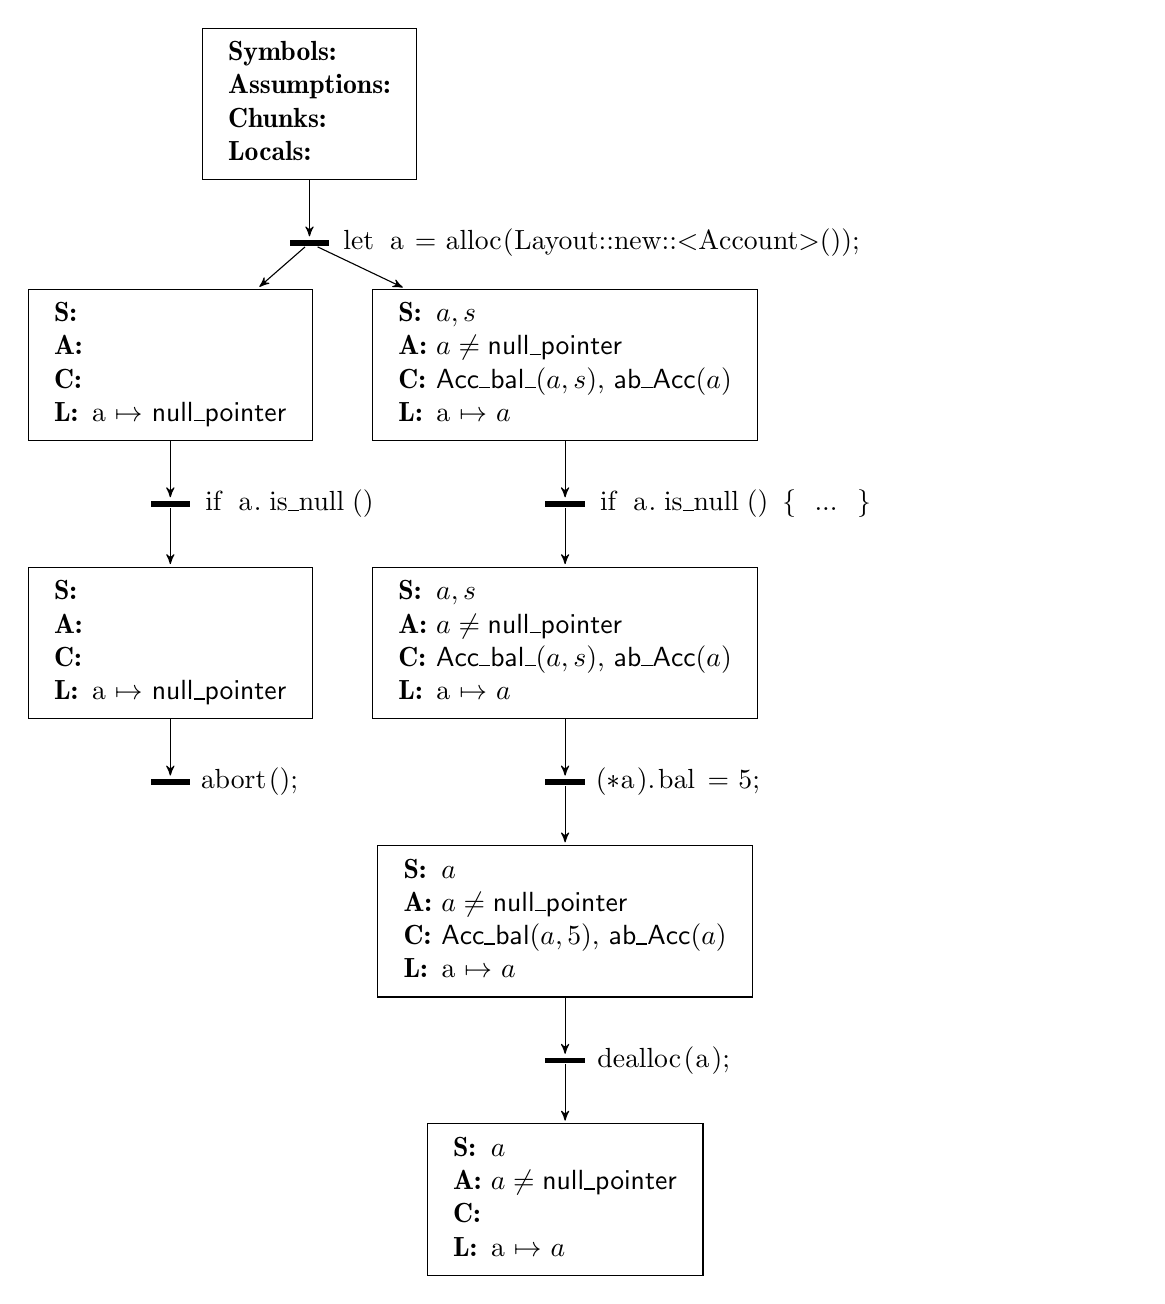
\begin{tikzpicture}
\node [state] (s1) {\begin{tabular}{l l}
\textbf{Symbols:}\\
\textbf{Assumptions:}\\
\textbf{Chunks:}\\
\textbf{Locals:}\\
\end{tabular}};
\node [transitionV] (t1) [below=of s1, label=right:\parbox{10cm}{\lstinline|let a = alloc(Layout::new::<Account>());|}] {}
  edge [pre] (s1);

\node [state] (s22) [below right=of t1] {\begin{tabular}{l @{\ } l}
\textbf{S:} & $\mathsfsl{a}, \mathsfsl{s}$\\
\textbf{A:} & $\mathsfsl{a} \neq \mathsf{null\_pointer}$\\
\textbf{C:} & $\mathsf{Acc\_bal\_}(\mathsfsl{a}, \mathsfsl{s})$, $\mathsf{ab\_Acc}(\mathsfsl{a})$\\
\textbf{L:} & \lstinline|a| $\mapsto$ $\mathsfsl{a}$
\end{tabular}}
  edge [pre] (t1);

\node [state] (s21) [left=of s22] {\begin{tabular}{l @{\ } l}
\textbf{S:}\\
\textbf{A:}\\
\textbf{C:}\\
\textbf{L:} & \lstinline|a| $\mapsto$ $\mathsf{null\_pointer}$
\end{tabular}}
  edge [pre] (t1);
\node [transitionV] (t21) [below=of s21, label=right:\parbox{5cm}{\lstinline|if a.is_null()|}] {}
  edge [pre] (s21);
\node [state] (s31) [below=of t21] {\begin{tabular}{l @{\ } l}
\textbf{S:}\\
\textbf{A:}\\
\textbf{C:}\\
\textbf{L:} & \lstinline|a| $\mapsto$ $\mathsf{null\_pointer}$
\end{tabular}}
  edge [pre] (t21);
\node [transitionV] (t31) [below=of s31, label=right:\parbox{5cm}{\lstinline|abort();|}] {}
  edge [pre] (s31);

\node [transitionV] (t22) [below=of s22, label=right:\parbox{5cm}{\lstinline|if a.is_null() \{ ... \}|}] {}
  edge [pre] (s22);
\node [state] (s32) [below=of t22] {\begin{tabular}{l @{\ } l}
\textbf{S:} & $\mathsfsl{a}, \mathsfsl{s}$\\
\textbf{A:} & $\mathsfsl{a} \neq \mathsf{null\_pointer}$\\
\textbf{C:} & $\mathsf{Acc\_bal\_}(\mathsfsl{a}, \mathsfsl{s})$, $\mathsf{ab\_Acc}(\mathsfsl{a})$\\
\textbf{L:} & \lstinline|a| $\mapsto$ $\mathsfsl{a}$
\end{tabular}}
  edge [pre] (t22);
\node [transitionV] (t32) [below=of s32, label=right:\parbox{5cm}{\lstinline|(*a).bal = 5;|}] {}
  edge [pre] (s32);
\node [state] (s42) [below=of t32] {\begin{tabular}{l @{\ } l}
\textbf{S:} & $\mathsfsl{a}$\\
\textbf{A:} & $\mathsfsl{a} \neq \mathsf{null\_pointer}$\\
\textbf{C:} & $\mathsf{Acc\_bal}(\mathsfsl{a}, 5)$, $\mathsf{ab\_Acc}(\mathsfsl{a})$\\
\textbf{L:} & \lstinline|a| $\mapsto$ $\mathsfsl{a}$
\end{tabular}}
  edge [pre] (t32);
\node [transitionV] (t42) [below=of s42, label=right:\parbox{5cm}{\lstinline|dealloc(a);|}] {}
  edge [pre] (s42);
\node [state] (s52) [below=of t42] {\begin{tabular}{l @{\ } l}
\textbf{S:} & $\mathsfsl{a}$\\
\textbf{A:} & $\mathsfsl{a} \neq \mathsf{null\_pointer}$\\
\textbf{C:}\\
\textbf{L:} & \lstinline|a| $\mapsto$ $\mathsfsl{a}$
\end{tabular}}
  edge [pre] (t42);
\end{tikzpicture}
\end{center}
\caption{Symbolic execution tree of the program of Figure~\ref{figure:illegal-access1} (after uncommenting the \lstinline|if| statement). We abbreviate \textbf{Chunks} as \textbf{C}, \textbf{Locals} as \textbf{L}, \lstinline|Account| as \lstinline|Acc|, \lstinline|balance| as \lstinline|bal|, \lstinline|my_account| as \lstinline|a|, and $\mathsf{alloc\_block}$ as $\mathsf{ab}$. Note that the tree is shown fully: the \lstinline|alloc| node has only two child nodes: the second child node summarizes (practically) infinitely many corresponding child nodes from the concrete execution tree. We print symbols in slanted font ($\mathsfsl{a}$) to avoid confusion with similarly named local variables (\lstinline|a|).}\label{fig:symex-tree}
\end{figure}

\subsection{Exercise \ref{exercise:account}: account.rs}

\begin{lstlisting}
// verifast_options{ignore_unwind_paths}
use std::alloc::{Layout, alloc, handle_alloc_error, dealloc};

struct Account {
    balance: i32,
}

impl Account {

    unsafe fn create() -> *mut Account
    //@ req true;
    //@ ens Account_balance(result, 0) &*& alloc_block_Account(result);
    {
        let my_account = alloc(Layout::new::<Account>()) as *mut Account;
        if my_account.is_null() {
            handle_alloc_error(Layout::new::<Account>());
        }
        (*my_account).balance = 0;
        my_account
    }

    unsafe fn set_balance(my_account: *mut Account, new_balance: i32)
    //@ req Account_balance(my_account, _);
    //@ ens Account_balance(my_account, new_balance);
    {
        (*my_account).balance = new_balance;
    }

    unsafe fn dispose(my_account: *mut Account)
    //@ req Account_balance(my_account, _) &*& alloc_block_Account(my_account);
    //@ ens true;
    {
        dealloc(my_account as *mut u8, Layout::new::<Account>());
    }

}

fn main()
//@ req true;
//@ ens true;
{
    unsafe {
        let my_account = Account::create();
        Account::set_balance(my_account, 5);
        Account::dispose(my_account);
    }
}
\end{lstlisting}

\subsection{Exercise \ref{exercise:deposit}: deposit.rs}

\begin{lstlisting}
unsafe fn deposit(my_account: *mut Account, amount: i32)
//@ req Account_balance(my_account, ?theBalance);
//@ ens Account_balance(my_account, theBalance + amount);
{
    (*my_account).balance += amount;
}
\end{lstlisting}

\subsection{Exercise \ref{exercise:limit}: limit.rs}

\begin{lstlisting}
// verifast_options{ignore_unwind_paths disable_overflow_check}
use std::alloc::{Layout, alloc, handle_alloc_error, dealloc};
//@ use std::alloc::{alloc_block, Layout};

struct Account {
    limit: i32,
    balance: i32,
}

impl Account {

    unsafe fn create(limit: i32) -> *mut Account
    //@ req limit <= 0;
    //@ ens (*result).limit |-> limit &*& (*result).balance |-> 0 &*& alloc_block_Account(result);
    {
        let my_account = alloc(Layout::new::<Account>()) as *mut Account;
        if my_account.is_null() {
            handle_alloc_error(Layout::new::<Account>());
        }
        (*my_account).limit = limit;
        (*my_account).balance = 0;
        my_account
    }

    unsafe fn get_balance(my_account: *mut Account) -> i32
    //@ req (*my_account).balance |-> ?theBalance;
    //@ ens (*my_account).balance |-> theBalance &*& result == theBalance;
    {
        (*my_account).balance
    }

    unsafe fn deposit(my_account: *mut Account, amount: i32)
    //@ req (*my_account).balance |-> ?theBalance;
    //@ ens (*my_account).balance |-> theBalance + amount;
    {
        (*my_account).balance += amount;
    }

    unsafe fn withdraw(my_account: *mut Account, amount: i32) -> i32
    //@ req (*my_account).limit |-> ?limit &*& (*my_account).balance |-> ?balance &*& 0 <= amount;
    /*@
    ens (*my_account).limit |-> limit &*& (*my_account).balance |-> balance - result &*&
        result == if balance - amount < limit { balance - limit } else { amount };
    @*/
    {
        let result =
            if (*my_account).balance - amount < (*my_account).limit {
                (*my_account).balance - (*my_account).limit
            } else {
                amount
            };
        (*my_account).balance -= result;
        result
    }

    unsafe fn dispose(my_account: *mut Account)
    //@ req (*my_account).limit |-> _ &*& (*my_account).balance |-> _ &*& alloc_block_Account(my_account);
    //@ ens true;
    {
        dealloc(my_account as *mut u8, Layout::new::<Account>());
    }

}
\end{lstlisting}

\subsection{Exercise \ref{exercise:pred}: pred.rs}

\begin{lstlisting}
// verifast_options{ignore_unwind_paths disable_overflow_check}
use std::alloc::{Layout, alloc, handle_alloc_error, dealloc};
//@ use std::alloc::{alloc_block, Layout};

struct Account {
    limit: i32,
    balance: i32,
}

/*@

pred Account_pred(my_account: *mut Account, theLimit: i32, theBalance: i32) =
    (*my_account).limit |-> theLimit &*& (*my_account).balance |-> theBalance &*&
    alloc_block_Account(my_account);

@*/

impl Account {

    unsafe fn create(limit: i32) -> *mut Account
    //@ req limit <= 0;
    //@ ens Account_pred(result, limit, 0);
    {
        let my_account = alloc(Layout::new::<Account>()) as *mut Account;
        if my_account.is_null() {
            handle_alloc_error(Layout::new::<Account>());
        }
        (*my_account).limit = limit;
        (*my_account).balance = 0;
        //@ close Account_pred(my_account, limit, 0);
        my_account
    }

    unsafe fn get_balance(my_account: *mut Account) -> i32
    //@ req Account_pred(my_account, ?limit, ?balance);
    //@ ens Account_pred(my_account, limit, balance) &*& result == balance;
    {
        //@ open Account_pred(my_account, limit, balance);
        let result = (*my_account).balance;
        //@ close Account_pred(my_account, limit, balance);
        result
    }

    unsafe fn deposit(my_account: *mut Account, amount: i32)
    //@ req Account_pred(my_account, ?limit, ?balance) &*& 0 <= amount;
    //@ ens Account_pred(my_account, limit, balance + amount);
    {
        //@ open Account_pred(my_account, limit, balance);
        (*my_account).balance += amount;
        //@ close Account_pred(my_account, limit, balance + amount);
    }

    unsafe fn withdraw(my_account: *mut Account, amount: i32) -> i32
    //@ req Account_pred(my_account, ?limit, ?balance) &*& 0 <= amount;
    /*@
    ens Account_pred(my_account, limit, balance - result) &*&
        result == if balance - amount < limit { balance - limit } else { amount };
    @*/
    {
        //@ open Account_pred(my_account, limit, balance);
        let result =
            if (*my_account).balance - amount < (*my_account).limit {
                (*my_account).balance - (*my_account).limit
            } else {
                amount
            };
        (*my_account).balance -= result;
        //@ close Account_pred(my_account, limit, balance - result);
        result
    }

    unsafe fn dispose(my_account: *mut Account)
    //@ req Account_pred(my_account, _, _);
    //@ ens true;
    {
        //@ open Account_pred(my_account, _, _);
        dealloc(my_account as *mut u8, Layout::new::<Account>());
    }

}

fn main()
//@ req true;
//@ ens true;
{
    unsafe {
        let my_account = Account::create(-100);
        Account::deposit(my_account, 200);
        let w1 = Account::withdraw(my_account, 50);
        std::hint::assert_unchecked(w1 == 50);
        let b1 = Account::get_balance(my_account);
        std::hint::assert_unchecked(b1 == 150);
        let w2 = Account::withdraw(my_account, 300);
        std::hint::assert_unchecked(w2 == 250);
        let b2 = Account::get_balance(my_account);
        std::hint::assert_unchecked(b2 == -100);
        Account::dispose(my_account);
    }
}
\end{lstlisting}

\subsection{Exercise
\ref{exercise:stack}: stack.rs}\label{solution:stack}

\begin{lstlisting}
// verifast_options{ignore_unwind_paths}
use std::alloc::{Layout, alloc, handle_alloc_error, dealloc};
//@ use std::alloc::{Layout, alloc_block};

struct Node {
    next: *mut Node,
    value: i32,
}

struct Stack {
    head: *mut Node,
}

/*@

pred Nodes(node: *mut Node, count: i32) =
    if node == 0 {
        count == 0
    } else {
        0 < count &*&
        (*node).next |-> ?next &*&
        (*node).value |-> ?value &*&
        alloc_block_Node(node) &*&
        Nodes(next, count - 1)
    };

pred Stack(stack: *mut Stack, count: i32) =
    (*stack).head |-> ?head &*&
    alloc_block_Stack(stack) &*&
    0 <= count &*&
    Nodes(head, count);

@*/

impl Stack {

    unsafe fn create() -> *mut Stack
    //@ req true;
    //@ ens Stack(result, 0);
    {
        let stack = alloc(Layout::new::<Stack>()) as *mut Stack;
        if stack.is_null() {
            handle_alloc_error(Layout::new::<Stack>());
        }
        (*stack).head = std::ptr::null_mut();
        //@ close Nodes(0, 0);
        //@ close Stack(stack, 0);
        stack
    }

    unsafe fn push(stack: *mut Stack, value: i32)
    //@ req Stack(stack, ?count);
    //@ ens Stack(stack, count + 1);
    {
        //@ open Stack(stack, count);
        let n = alloc(Layout::new::<Node>()) as *mut Node;
        if n.is_null() {
            handle_alloc_error(Layout::new::<Node>());
        }
        (*n).next = (*stack).head;
        (*n).value = value;
        (*stack).head = n;
        //@ close Nodes(n, count + 1);
        //@ close Stack(stack, count + 1);
    }

    unsafe fn pop(stack: *mut Stack) -> i32
    //@ req Stack(stack, ?count) &*& 0 < count;
    //@ ens Stack(stack, count - 1);
    {
        //@ open Stack(stack, count);
        let head = (*stack).head;
        //@ open Nodes(head, count);
        let result = (*head).value;
        (*stack).head = (*head).next;
        dealloc(head as *mut u8, Layout::new::<Node>());
        //@ close Stack(stack, count - 1);
        result
    }

    unsafe fn dispose(stack: *mut Stack)
    //@ req Stack(stack, 0);
    //@ ens true;
    {
        //@ open Stack(stack, 0);
        //@ open Nodes(_, _);
        dealloc(stack as *mut u8, Layout::new::<Stack>());
    }

}

fn main()
//@ req true;
//@ ens true;
{
    unsafe {
        let s = Stack::create();
        Stack::push(s, 10);
        Stack::push(s, 20);
        Stack::pop(s);
        Stack::pop(s);
        Stack::dispose(s);
    }
}
\end{lstlisting}

\subsection{Exercise
\ref{exercise:dispose}: dispose.rs}\label{solution:dispose}

\begin{lstlisting}
unsafe fn dispose_nodes(n: *mut Node)
//@ req Nodes(n, _);
//@ ens true;
{
    //@ open Nodes(n, _);
    if !n.is_null() {
        dispose_nodes((*n).next);
        dealloc(n as *mut u8, Layout::new::<Node>());
    }
}

impl Stack {

    unsafe fn dispose(stack: *mut Stack)
    //@ req Stack(stack, _);
    //@ ens true;
    {
        //@ open Stack(stack, _);
        dispose_nodes((*stack).head);
        dealloc(stack as *mut u8, Layout::new::<Stack>());
    }

}
\end{lstlisting}

\subsection{Exercise
\ref{exercise:sum}: sum.rs}\label{solution:sum}

\begin{lstlisting}
unsafe fn get_nodes_sum(nodes: *mut Node) -> i32
//@ req Nodes(nodes, ?count);
//@ ens Nodes(nodes, count);
{
    let mut result = 0;
    //@ open Nodes(nodes, count);
    if !nodes.is_null() {
        result = get_nodes_sum((*nodes).next);
        result += (*nodes).value;
    }
    //@ close Nodes(nodes, count);
    result
}

impl Stack {

    unsafe fn get_sum(stack: *mut Stack) -> i32
    //@ req Stack(stack, ?count);
    //@ ens Stack(stack, count);
    {
        //@ open Stack(stack, count);
        let result = get_nodes_sum((*stack).head);
        //@ close Stack(stack, count);
        result
    }

}
\end{lstlisting}

\subsection{Exercise
\ref{exercise:popn}: popn.rs}\label{solution:popn}

\begin{lstlisting}
unsafe fn popn(stack: *mut Stack, n: i32)
//@ req Stack(stack, ?count) &*& 0 <= n &*& n <= count;
//@ ens Stack(stack, count - n);
{
    let mut i = 0;
    loop {
        //@ inv Stack(stack, count - i) &*& i <= n;
        if i == n {
            break;
        }
        Stack::pop(stack);
        i += 1;
    }
}
\end{lstlisting}

\subsection{Exercise
\ref{exercise:values}: values.rs}\label{solution:values}

\begin{lstlisting}
// verifast_options{ignore_unwind_paths}
use std::alloc::{Layout, alloc, handle_alloc_error, dealloc};
//@ use std::alloc::{Layout, alloc_block};

struct Node {
    next: *mut Node,
    value: i32,
}

struct Stack {
    head: *mut Node,
}

/*@

inductive i32s = i32s_nil | i32s_cons(i32, i32s);

pred Nodes(node: *mut Node, values: i32s) =
    if node == 0 {
        values == i32s_nil
    } else {
        (*node).next |-> ?next &*& (*node).value |-> ?value &*&
        alloc_block_Node(node) &*& Nodes(next, ?values0) &*&
        values == i32s_cons(value, values0)
    };

pred Stack(stack: *mut Stack, values: i32s) =
    (*stack).head |-> ?head &*& alloc_block_Stack(stack) &*& Nodes(head, values);

@*/

impl Stack {

    unsafe fn create() -> *mut Stack
    //@ req true;
    //@ ens Stack(result, i32s_nil);
    {
        let stack = alloc(Layout::new::<Stack>()) as *mut Stack;
        if stack.is_null() {
            handle_alloc_error(Layout::new::<Stack>());
        }
        (*stack).head = std::ptr::null_mut();
        //@ close Nodes(0, i32s_nil);
        //@ close Stack(stack, i32s_nil);
        stack
    }
    
    unsafe fn push(stack: *mut Stack, value: i32)
    //@ req Stack(stack, ?values);
    //@ ens Stack(stack, i32s_cons(value, values));
    {
        //@ open Stack(stack, values);
        let n = alloc(Layout::new::<Node>()) as *mut Node;
        if n.is_null() {
            handle_alloc_error(Layout::new::<Node>());
        }
        (*n).next = (*stack).head;
        (*n).value = value;
        (*stack).head = n;
        //@ close Nodes(n, i32s_cons(value, values));
        //@ close Stack(stack, i32s_cons(value, values));
    }

    unsafe fn dispose(stack: *mut Stack)
    //@ req Stack(stack, i32s_nil);
    //@ ens true;
    {
        //@ open Stack(stack, i32s_nil);
        //@ open Nodes(_, _);
        dealloc(stack as *mut u8, Layout::new::<Stack>());
    }

}
\end{lstlisting}

\subsection{Exercise
\ref{exercise:fixpoints}: fixpoints.rs}\label{solution:fixpoints}

\begin{lstlisting}
unsafe fn pop(stack: *mut Stack) -> i32
//@ req Stack(stack, ?values) &*& values != i32s_nil;
//@ ens Stack(stack, i32s_tail(values)) &*& result == i32s_head(values);
{
    //@ open Stack(stack, values);
    let head = (*stack).head;
    //@ open Nodes(head, values);
    let result = (*head).value;
    (*stack).head = (*head).next;
    dealloc(head as *mut u8, Layout::new::<Node>());
    //@ close Stack(stack, i32s_tail(values));
    result
}
\end{lstlisting}

\subsection{Exercise
\ref{exercise:sum_full}: sum\_full.rs}\label{solution:sum_full}

\begin{lstlisting}
/*@

fix i32s_sum(values: i32s) -> i32 {
    match values {
        i32s_nil => 0,
        i32s_cons(value, values0) => value + i32s_sum(values0),
    }
}

@*/

unsafe fn get_nodes_sum(node: *mut Node) -> i32
//@ req Nodes(node, ?values);
//@ ens Nodes(node, values) &*& result == i32s_sum(values);
{
    //@ open Nodes(node, values);
    let mut result = 0;
    if !node.is_null() {
        let tail_sum = get_nodes_sum((*node).next);
        result = (*node).value + tail_sum;
    }
    //@ close Nodes(node, values);
    result
}

impl Stack {

    unsafe fn get_sum(stack: *mut Stack) -> i32
    //@ req Stack(stack, ?values);
    //@ ens Stack(stack, values) &*& result == i32s_sum(values);
    {
        //@ open Stack(stack, values);
        let result = get_nodes_sum((*stack).head);
        //@ close Stack(stack, values);
        result
    }

}
\end{lstlisting}

\subsection{Exercise
\ref{exercise:lemma}: lemma.rs}\label{solution:lemma}

\begin{lstlisting}
lem lseg_to_Nodes_lemma(first: *mut Node)
    req lseg(first, 0, ?count);
    ens Nodes(first, count);
{
    open lseg(first, 0, count);
    if first != 0 {
        lseg_to_Nodes_lemma((*first).next);
    }
    close Nodes(first, count);
}
\end{lstlisting}

\subsection{Exercise
\ref{exercise:push_all}: push\_all.rs}\label{solution:push_all}

\begin{lstlisting}
/*@

lem lseg_append_lemma(first: *mut Node)
    req lseg(first, ?n, ?count) &*& lseg(n, 0, ?count0);
    ens lseg(first, 0, count + count0);
{
    open lseg(first, n, count);
    if first != n {
        open lseg(n, 0, count0);
        close lseg(n, 0, count0);
        lseg_append_lemma((*first).next);
        close lseg(first, 0, count + count0);
    }
}

@*/

impl Stack {
    unsafe fn push_all(stack: *mut Stack, other: *mut Stack)
    //@ req Stack(stack, ?count) &*& Stack(other, ?count0);
    //@ ens Stack(stack, count0 + count);
    {
        //@ open Stack(stack, count);
        //@ Nodes_to_lseg_lemma((*stack).head);
        //@ open Stack(other, count0);
        //@ Nodes_to_lseg_lemma((*other).head);
        let head0 = (*other).head;
        dealloc(other as *mut u8, Layout::new::<Stack>());
        let mut n = head0;
        //@ open lseg(head0, 0, count0);
        if !n.is_null() {
            //@ close lseg(head0, head0, 0);
            loop {
                /*@
                inv lseg(head0, n, ?count1) &*& n != 0 &*& (*n).value |-> ?n_value &*& 
                    (*n).next |-> ?next &*&
                    alloc_block_Node(n) &*&
                    lseg(next, 0, count0 - count1 - 1);
                @*/
                if (*n).next.is_null() {
                    break;
                }
                n = (*n).next;
                //@ lseg_add_lemma(head0);
                //@ open lseg(next, 0, count0 - count1 - 1);
            }
            //@ open lseg(0, 0, _);
            (*n).next = (*stack).head;
            //@ lseg_add_lemma(head0);
            //@ lseg_append_lemma(head0);
            (*stack).head = head0;
        }
        //@ lseg_to_Nodes_lemma((*stack).head);
        //@ close Stack(stack, count0 + count);
    }
}
\end{lstlisting}

\subsection{Exercise
\ref{exercise:reverse}: reverse.rs}\label{solution:reverse}

\begin{lstlisting}
fix i32s_append(values1: i32s, values2: i32s) -> i32s {
    match values1 {
        i32s_nil => values2,
        i32s_cons(h, t) => i32s_cons(h, i32s_append(t, values2)),
    }
}

lem i32s_append_nil_lemma(values: i32s)
    req true;
    ens i32s_append(values, i32s_nil) == values;
{
    match values {
        i32s_nil => {}
        i32s_cons(h, t) => {
            i32s_append_nil_lemma(t);
        }
    }
}

lem i32s_append_assoc_lemma(values1: i32s, values2: i32s, values3: i32s)
    req true;
    ens i32s_append(i32s_append(values1, values2), values3)
        == i32s_append(values1, i32s_append(values2, values3));
{
    match values1 {
        i32s_nil => {}
        i32s_cons(h, t) => {
            i32s_append_assoc_lemma(t, values2, values3);
        }
    }
}

fix i32s_reverse(values: i32s) -> i32s {
    match values {
        i32s_nil => i32s_nil,
        i32s_cons(h, t) => i32s_append(i32s_reverse(t), i32s_cons(h, i32s_nil))
    }
}

@*/

impl Stack {
    unsafe fn reverse(stack: *mut Stack)
    //@ req Stack(stack, ?values);
    //@ ens Stack(stack, i32s_reverse(values));
    {
        //@ open Stack(stack, values);
        let mut n = (*stack).head;
        let mut m = std::ptr::null_mut();
        //@ close Nodes(m, i32s_nil);
        //@ i32s_append_nil_lemma(i32s_reverse(values));
        loop {
            /*@
            inv Nodes(m, ?values1) &*& Nodes(n, ?values2) &*&
                i32s_reverse(values) == i32s_append(i32s_reverse(values2), values1);
            @*/
            if n.is_null() {
                break;
            }
            //@ open Nodes(n, values2);
            let next = (*n).next;
            //@ assert Nodes(next, ?values2_tail) &*& (*n).value |-> ?value;
            (*n).next = m;
            m = n;
            n = next;
            //@ close Nodes(m, i32s_cons(value, values1));
            //@ i32s_append_assoc_lemma(i32s_reverse(values2_tail), i32s_cons(value, i32s_nil), values1);
        }
        //@ open Nodes(n, _);
        (*stack).head = m;
        //@ close Stack(stack, i32s_reverse(values));
    }
}
\end{lstlisting}

\subsection{Exercise
\ref{exercise:filter}: filter.rs}\label{solution:filter}

\begin{lstlisting}
// verifast_options{ignore_unwind_paths}
use std::alloc::{Layout, alloc, handle_alloc_error, dealloc};
//@ use std::alloc::{Layout, alloc_block};

struct Node {
    next: *mut Node,
    value: i32,
}

struct Stack {
    head: *mut Node,
}

/*@

pred Nodes(node: *mut Node, count: i32) =
    if node == 0 {
        count == 0
    } else {
        0 < count &*&
        (*node).next |-> ?next &*& (*node).value |-> ?value &*&
        alloc_block_Node(node) &*& Nodes(next, count - 1)
    };

pred Stack(stack: *mut Stack, count: i32) =
    (*stack).head |-> ?head &*& alloc_block_Stack(stack) &*& 0 <= count &*& Nodes(head, count);

fn_type I32Predicate() = unsafe fn(x: i32) -> bool;
    req true;
    ens true;

@*/

type I32Predicate = unsafe fn(i32) -> bool;

unsafe fn filter_nodes(n: *mut Node, p: I32Predicate) -> *mut Node
//@ req Nodes(n, _) &*& [_]is_I32Predicate(p);
//@ ens Nodes(result, _);
{
    if n.is_null() {
        std::ptr::null_mut()
    } else {
        //@ open Nodes(n, _);
        let keep = p((*n).value);
        let next;
        if keep {
            next = filter_nodes((*n).next, p);
            //@ open Nodes(next, ?count);
            //@ close Nodes(next, count);
            (*n).next = next;
            //@ close Nodes(n, count + 1);
            n
        } else {
            next = (*n).next;
            dealloc(n as *mut u8, Layout::new::<Node>());
            let result = filter_nodes(next, p);
            result
        }
    }
}

unsafe fn dispose_nodes(n: *mut Node)
//@ req Nodes(n, _);
//@ ens true;
{
    //@ open Nodes(n, _);
    if !n.is_null() {
        dispose_nodes((*n).next);
        dealloc(n as *mut u8, Layout::new::<Node>());
    }
}

impl Stack {

    unsafe fn create() -> *mut Stack
    //@ req true;
    //@ ens Stack(result, 0);
    {
        let stack = alloc(Layout::new::<Stack>()) as *mut Stack;
        if stack.is_null() {
            handle_alloc_error(Layout::new::<Stack>());
        }
        (*stack).head = std::ptr::null_mut();
        //@ close Nodes(0, 0);
        //@ close Stack(stack, 0);
        stack
    }
    
    unsafe fn push(stack: *mut Stack, value: i32)
    //@ req Stack(stack, ?count);
    //@ ens Stack(stack, count + 1);
    {
        //@ open Stack(stack, count);
        let n = alloc(Layout::new::<Node>()) as *mut Node;
        if n.is_null() {
            handle_alloc_error(Layout::new::<Node>());
        }
        (*n).next = (*stack).head;
        (*n).value = value;
        (*stack).head = n;
        //@ close Nodes(n, count + 1);
        //@ close Stack(stack, count + 1);
    }

    unsafe fn pop(stack: *mut Stack) -> i32
    //@ req Stack(stack, ?count) &*& 0 < count;
    //@ ens Stack(stack, count - 1);
    {
        //@ open Stack(stack, count);
        let head = (*stack).head;
        //@ open Nodes(head, count);
        let result = (*head).value;
        (*stack).head = (*head).next;
        dealloc(head as *mut u8, Layout::new::<Node>());
        //@ close Stack(stack, count - 1);
        result
    }
    
    unsafe fn filter(stack: *mut Stack, p: I32Predicate)
    //@ req Stack(stack, _) &*& [_]is_I32Predicate(p);
    //@ ens Stack(stack, _);
    {
        //@ open Stack(stack, _);
        let head = filter_nodes((*stack).head, p);
        //@ assert Nodes(head, ?count);
        (*stack).head = head;
        //@ open Nodes(head, count);
        //@ close Nodes(head, count);
        //@ close Stack(stack, count);
    }
    
    unsafe fn dispose(stack: *mut Stack)
    //@ req Stack(stack, _);
    //@ ens true;
    {
        //@ open Stack(stack, _);
        dispose_nodes((*stack).head);
        dealloc(stack as *mut u8, Layout::new::<Stack>());
    }

}

unsafe fn neq_20(x: i32) -> bool
//@ req true;
//@ ens true;
{
    x != 20
}

fn main()
//@ req true;
//@ ens true;
{
    unsafe {
        let s = Stack::create();
        Stack::push(s, 10);
        Stack::push(s, 20);
        /*@
        produce_fn_ptr_chunk I32Predicate(neq_20)()(x) {
            call();
        }
        @*/
        Stack::filter(s, neq_20);
        Stack::dispose(s);
    }
}
\end{lstlisting}

\subsection{Exercise
\ref{exercise:byref}: byref.rs}\label{solution:byref}

\begin{lstlisting}
unsafe fn filter_nodes(n: *mut *mut Node, p: I32Predicate)
//@ req *n |-> ?node &*& Nodes(node, _) &*& [_]is_I32Predicate(p);
//@ ens *n |-> ?node0 &*& Nodes(node0, _);
{
    if !(*n).is_null() {
        //@ open Nodes(node, _);
        let keep = p((**n).value);
        if keep {
            //@ open Node_next(node, _);
            filter_nodes(&raw mut (**n).next, p);
            //@ close Node_next(node, ?next);
            //@ open Nodes(next, ?count);
            //@ close Nodes(next, count);
            //@ close Nodes(node, count + 1);
        } else {
            let next_ = (**n).next;
            dealloc(*n as *mut u8, Layout::new::<Node>());
            *n = next_;
            filter_nodes(n, p);
        }
    }
}
\end{lstlisting}

\subsection{Exercise \ref{exercise:map}:
map.rs}\label{solution:map}

\begin{lstlisting}
/*@
fn_type I32Func(data_pred: pred(*mut u8)) = unsafe fn(data: *mut u8, x: i32) -> i32;
    req data_pred(data);
    ens data_pred(data);
@*/

type I32Func = unsafe fn(*mut u8, i32) -> i32;

unsafe fn map_nodes(n: *mut Node, f: I32Func, data: *mut u8)
//@ req Nodes(n, ?count) &*& [_]is_I32Func(f, ?data_pred) &*& data_pred(data);
//@ ens Nodes(n, count) &*& data_pred(data);
{
    //@ open Nodes(n, _);
    if !n.is_null() {
        let y = f(data, (*n).value);
        (*n).value = y;
        map_nodes((*n).next, f, data);
    }
    //@ close Nodes(n, count);
}

impl Stack {
    unsafe fn map(stack: *mut Stack, f: I32Func, data: *mut u8)
    //@ req Stack(stack, ?count) &*& [_]is_I32Func(f, ?data_pred) &*& data_pred(data);
    //@ ens Stack(stack, count) &*& data_pred(data);
    {
        //@ open Stack(stack, _);
        map_nodes((*stack).head, f, data);
        //@ close Stack(stack, count);
    }
}
\end{lstlisting}

\subsection{Exercise \ref{exercise:foreach}:
foreach.c}\label{solution:foreach}

\begin{lstlisting}
char input_char();
    //@ requires true;
    //@ ensures true;

int input_int();
    //@ requires true;
    //@ ensures true;

void output_int(int x);
    //@ requires true;
    //@ ensures true;

struct vector {
    int x;
    int y;
};

//@ predicate vector(struct vector *v) = v->x |-> _ &*& v->y |-> _ &*& malloc_block_vector(v);

struct vector *create_vector(int x, int y)
    //@ requires true;
    //@ ensures vector(result);
{
    struct vector *result = malloc(sizeof(struct vector));
    if (result == 0) abort();
    result->x = x;
    result->y = y;
    //@ close vector(result);
    return result;
}

int main()
    //@ requires true;
    //@ ensures true;
{
    struct stack *s = create_stack();
    //@ close foreach(nil, vector);
    while (true)
        //@ invariant stack(s, ?values) &*& foreach(values, vector);
    {
        char c = input_char();
        if (c == 'p') {
            int x = input_int();
            int y = input_int();
            struct vector *v = create_vector(x, y);
            stack_push(s, v);
            //@ close foreach(cons(v, values), vector);
        } else if (c == '+') {
            bool empty = stack_is_empty(s);
            if (empty) abort();
            struct vector *v1 = stack_pop(s);
            //@ open foreach(values, vector);
            //@ open vector(head(values));
            empty = stack_is_empty(s);
            if (empty) abort();
            struct vector *v2 = stack_pop(s);
            //@ open foreach(tail(values), vector);
            //@ open vector(head(tail(values)));
            struct vector *sum = create_vector(v1->x + v2->x, v1->y + v2->y);
            free(v1);
            free(v2);
            stack_push(s, sum);
            //@ close foreach(cons(sum, tail(tail(values))), vector);
        } else if (c == '=') {
            bool empty = stack_is_empty(s);
            if (empty) abort();
            struct vector *v = stack_pop(s);
            //@ open foreach(values, vector);
            //@ open vector(head(values));
            output_int(v->x);
            output_int(v->y);
            free(v);
        } else {
            abort();
        }
    }
}
\end{lstlisting}

\subsection{Exercise \ref{exercise:predctors}:
predctors.c}\label{solution:predctors}

\begin{lstlisting}
struct vector {
    int x;
    int y;
};

/*@
predicate_ctor vector(int limit)(struct vector *v) =
    v->x |-> ?x &*& v->y |-> ?y &*& malloc_block_vector(v) &*& x * x + y * y <= limit * limit;
@*/

struct vector *create_vector(int limit, int x, int y)
    //@ requires true;
    //@ ensures vector(limit)(result);
{
    if (x * x + y * y > limit * limit) abort();
    struct vector *result = malloc(sizeof(struct vector));
    if (result == 0) abort();
    result->x = x;
    result->y = y;
    //@ close vector(limit)(result);
    return result;
}

int main()
    //@ requires true;
    //@ ensures true;
{
    int limit = input_int();
    struct stack *s = create_stack();
    //@ close foreach(nil, vector(limit));
    while (true)
        //@ invariant stack(s, ?values) &*& foreach(values, vector(limit));
    {
        char c = input_char();
        if (c == 'p') {
            int x = input_int();
            int y = input_int();
            struct vector *v = create_vector(limit, x, y);
            stack_push(s, v);
            //@ close foreach(cons(v, values), vector(limit));
        } else if (c == '+') {
            bool empty = stack_is_empty(s);
            if (empty) abort();
            struct vector *v1 = stack_pop(s);
            //@ open foreach(values, vector(limit));
            //@ open vector(limit)(head(values));
            empty = stack_is_empty(s);
            if (empty) abort();
            struct vector *v2 = stack_pop(s);
            //@ open foreach(tail(values), vector(limit));
            //@ open vector(limit)(head(tail(values)));
            struct vector *sum = create_vector(limit, v1->x + v2->x, v1->y + v2->y);
            free(v1);
            free(v2);
            stack_push(s, sum);
            //@ close foreach(cons(sum, tail(tail(values))), vector(limit));
        } else if (c == '=') {
            bool empty = stack_is_empty(s);
            if (empty) abort();
            struct vector *v = stack_pop(s);
            //@ open foreach(values, vector(limit));
            //@ open vector(limit)(head(values));
            int x = v->x;
            int y = v->y;
            free(v);
            assert(x * x + y * y <= limit * limit);
            output_int(x);
            output_int(y);
        } else {
            abort();
        }
    }
}
\end{lstlisting}

\subsection{Exercise \ref{exercise:threads0}:
threads0.c}\label{solution:threads0}

\begin{lstlisting}
#include "stdlib.h"
#include "malloc.h"

int rand();
    //@ requires true;
    //@ ensures true;

int fac(int x)
    //@ requires true;
    //@ ensures true;
{
    int result = 1;
    while (x > 1)
        //@ invariant true;
    {
        result = result * x;
        x = x - 1;
    }
    return result;
}

struct tree {
    struct tree *left;
    struct tree *right;
    int value;
};

/*@ predicate tree(struct tree *t, int depth) =
    t == 0 ?
        depth == 0
    :
        t->left |-> ?left &*& t->right |-> ?right &*& t->value |-> ?value &*&
        malloc_block_tree(t) &*& tree(left, depth - 1) &*& tree(right, depth - 1);
@*/

struct tree *make_tree(int depth)
    //@ requires true;
    //@ ensures tree(result, depth);
{
    if (depth == 0) {
        //@ close tree(0, 0);
        return 0;
    } else {
        struct tree *left = make_tree(depth - 1);
        struct tree *right = make_tree(depth - 1);
        int value = rand();
        struct tree *t = malloc(sizeof(struct tree));
        if (t == 0) abort();
        t->left = left;
        t->right = right;
        t->value = value % 2000;
        //@ close tree(t, depth);
        return t;
    }
}

int tree_compute_sum_facs(struct tree *tree)
    //@ requires tree(tree, ?depth);
    //@ ensures tree(tree, depth);
{
    if (tree == 0) {
        return 1;
    } else {
        //@ open tree(tree, depth);
        int leftSum = tree_compute_sum_facs(tree->left);
        int rightSum = tree_compute_sum_facs(tree->right);
        int f = fac(tree->value);
        return leftSum + rightSum + f;
        //@ close tree(tree, depth);
    }
}

int main()
    //@ requires true;
    //@ ensures true;
{
    struct tree *tree = make_tree(22);
    int sum = tree_compute_sum_facs(tree);
    //@ leak tree(tree, _);
    return sum;
}
\end{lstlisting}

\subsection{Exercise \ref{exercise:threads}:
threads.c}\label{solution:threads}

\begin{lstlisting}
struct sum_data {
    struct thread *thread;
    struct tree *tree;
    int sum;
};

/*@

predicate_family_instance thread_run_pre(summator)(struct sum_data *data, any info) =
    data->tree |-> ?tree &*& tree(tree, _) &*& data->sum |-> _;
predicate_family_instance thread_run_post(summator)(struct sum_data *data, any info) =
    data->tree |-> ?tree &*& tree(tree, _) &*& data->sum |-> ?sum;

@*/

void summator(struct sum_data *data) //@ : thread_run_joinable
    //@ requires thread_run_pre(summator)(data, ?info);
    //@ ensures thread_run_post(summator)(data, info);
{
    //@ open thread_run_pre(summator)(data, info);
    int sum = tree_compute_sum_facs(data->tree);
    data->sum = sum;
    //@ close thread_run_post(summator)(data, info);
}

struct sum_data *start_sum_thread(struct tree *tree)
    //@ requires tree(tree, _);
    //@ ensures result->thread |-> ?t &*& thread(t, summator, result, _);
{
    struct sum_data *data = malloc(sizeof(struct sum_data));
    struct thread *t = 0;
    if (data == 0) abort();
    //@ leak malloc_block_sum_data(data);
    data->tree = tree;
    //@ close thread_run_pre(summator)(data, unit);
    t = thread_start_joinable(summator, data);
    data->thread = t;
    return data;
}

int join_sum_thread(struct sum_data *data)
    //@ requires data->thread |-> ?t &*& thread(t, summator, data, _);
    //@ ensures true;
{
    thread_join(data->thread);
    //@ open thread_run_post(summator)(data, _);
    return data->sum;
    //@ leak data->tree |-> ?tree &*& tree(tree, _) &*& data->sum |-> _ &*& data->thread |-> _;
}

int main()
    //@ requires true;
    //@ ensures true;
{
    struct tree *tree = make_tree(22);
    //@ open tree(tree, _);
    struct sum_data *leftData = start_sum_thread(tree->left);
    struct sum_data *rightData = start_sum_thread(tree->right);
    int sumLeft = join_sum_thread(leftData);
    int sumRight = join_sum_thread(rightData);
    int f = fac(tree->value);
    //@ leak tree->left |-> _ &*& tree->right |-> _ &*& tree->value |-> _ &*& malloc_block_tree(tree);
    return sumLeft + sumRight + f;
}
\end{lstlisting}

\subsection{Exercise \ref{exercise:fractions0}: fractions0.c}\label{solution:fractions0}

\begin{lstlisting}
typedef int fold_function(int acc, int x);
    //@ requires true;
    //@ ensures true;

int tree_fold(struct tree *tree, fold_function *f, int acc)
    //@ requires tree(tree, ?depth) &*& is_fold_function(f) == true;
    //@ ensures tree(tree, depth);
{
    if (tree == 0) {
        return acc;
    } else {
        //@ open tree(tree, depth);
        acc = tree_fold(tree->left, f, acc);
        acc = tree_fold(tree->right, f, acc);
        acc = f(acc, tree->value);
        return acc;
        //@ close tree(tree, depth);
    }
}

struct fold_data {
    struct thread *thread;
    struct tree *tree;
    fold_function *f;
    int acc;
};

/*@

predicate_family_instance thread_run_pre(folder)(struct fold_data *data, any info) =
    data->tree |-> ?tree &*& tree(tree, _) &*&
    data->f |-> ?f &*& is_fold_function(f) == true &*& data->acc |-> ?acc;
predicate_family_instance thread_run_post(folder)(struct fold_data *data, any info) =
    data->tree |-> ?tree &*& tree(tree, _) &*&
    data->f |-> ?f &*& is_fold_function(f) == true &*& data->acc |-> ?acc;

@*/

void folder(struct fold_data *data) //@ : thread_run_joinable
    //@ requires thread_run_pre(folder)(data, ?info);
    //@ ensures thread_run_post(folder)(data, info);
{
    //@ open thread_run_pre(folder)(data, info);
    int acc = tree_fold(data->tree, data->f, data->acc);
    data->acc = acc;
    //@ close thread_run_post(folder)(data, info);
}

struct fold_data *start_fold_thread(struct tree *tree, fold_function *f, int acc)
    //@ requires tree(tree, _) &*& is_fold_function(f) == true;
    //@ ensures result->thread |-> ?t &*& thread(t, folder, result, _);
{
    struct fold_data *data = malloc(sizeof(struct fold_data));
    struct thread *t = 0;
    if (data == 0) abort();
    //@ leak malloc_block_fold_data(data);
    data->tree = tree;
    data->f = f;
    data->acc = acc;
    //@ close thread_run_pre(folder)(data, unit);
    t = thread_start_joinable(folder, data);
    data->thread = t;
    return data;
}

int join_fold_thread(struct fold_data *data)
    //@ requires data->thread |-> ?t &*& thread(t, folder, data, _);
    //@ ensures true;
{
    thread_join(data->thread);
    //@ open thread_run_post(folder)(data, _);
    return data->acc;
    //@ leak data->tree |-> ?tree &*& [_]tree(tree, _);
    //@ leak data->f |-> _ &*& data->acc |-> _ &*& data->thread |-> _;
}

int sum_function(int acc, int x) //@ : fold_function
    //@ requires true;
    //@ ensures true;
{
    int f = fac(x);
    return acc + f;
}

int product_function(int acc, int x) //@ : fold_function
    //@ requires true;
    //@ ensures true;
{
    int f = fac(x);
    return acc * f;
}

int main()
    //@ requires true;
    //@ ensures true;
{
    struct tree *tree = make_tree(22);
    //@ open tree(tree, _);
    struct fold_data *leftData = start_fold_thread(tree->left, sum_function, 0);
    struct fold_data *rightData = start_fold_thread(tree->right, sum_function, 0);
    int sumLeft = join_fold_thread(leftData);
    int sumRight = join_fold_thread(rightData);
    int f = fac(tree->value);
    //@ leak tree->left |-> _ &*& tree->right |-> _ &*& tree->value |-> _ &*& malloc_block_tree(tree);
    return sumLeft + sumRight + f;
}
\end{lstlisting}

\subsection{Exercise \ref{exercise:fractions}:
fractions.c}\label{solution:fractions}

\begin{lstlisting}
/*@

predicate_family_instance thread_run_pre(folder)(struct fold_data *data, any info) =
    data->tree |-> ?tree &*& [1/2]tree(tree, _) &*&
    data->f |-> ?f &*& is_fold_function(f) == true &*& data->acc |-> ?acc;
predicate_family_instance thread_run_post(folder)(struct fold_data *data, any info) =
    data->tree |-> ?tree &*& [1/2]tree(tree, _) &*&
    data->f |-> ?f &*& is_fold_function(f) == true &*& data->acc |-> ?acc;

@*/

void folder(struct fold_data *data) //@ : thread_run_joinable
    //@ requires thread_run_pre(folder)(data, ?info);
    //@ ensures thread_run_post(folder)(data, info);
{
    //@ open thread_run_pre(folder)(data, info);
    int acc = tree_fold(data->tree, data->f, data->acc);
    data->acc = acc;
    //@ close thread_run_post(folder)(data, info);
}

struct fold_data *start_fold_thread(struct tree *tree, fold_function *f, int acc)
    //@ requires [1/2]tree(tree, _) &*& is_fold_function(f) == true;
    //@ ensures result->thread |-> ?t &*& thread(t, folder, result, _);
{
    struct fold_data *data = malloc(sizeof(struct fold_data));
    struct thread *t = 0;
    if (data == 0) abort();
    //@ leak malloc_block_fold_data(data);
    data->tree = tree;
    data->f = f;
    data->acc = acc;
    //@ close thread_run_pre(folder)(data, unit);
    t = thread_start_joinable(folder, data);
    data->thread = t;
    return data;
}

int join_fold_thread(struct fold_data *data)
    //@ requires data->thread |-> ?t &*& thread(t, folder, data, _);
    //@ ensures true;
{
    thread_join(data->thread);
    //@ open thread_run_post(folder)(data, _);
    return data->acc;
    //@ leak data->tree |-> ?tree &*& [_]tree(tree, _);
    //@ leak data->f |-> _ &*& data->acc |-> _ &*& data->thread |-> _;
}
\end{lstlisting}

\subsection{Exercise \ref{exercise:mutexes}:
mutexes.c}\label{solution:mutexes}

\begin{lstlisting}
#include "stdlib.h"
#include "threading.h"

void wait_for_pulse(int source);
    //@ requires true;
    //@ ensures true;

void sleep(int millis);
    //@ requires true;
    //@ ensures true;

void print_int(int n);
    //@ requires true;
    //@ ensures true;

struct counter {
    int count;
    struct mutex *mutex;
};

//@ predicate_ctor counter(struct counter *counter)() = counter->count |-> ?count;

struct count_pulses_data {
    struct counter *counter;
    int source;
};

/*@

predicate_family_instance thread_run_data(count_pulses)(struct count_pulses_data *data) =
    malloc_block_count_pulses_data(data) &*&
    data->counter |-> ?counter &*& data->source |-> ?source &*&
    [1/2]counter->mutex |-> ?mutex &*& [1/3]mutex(mutex, counter(counter));

@*/

void count_pulses(struct count_pulses_data *data) //@ : thread_run
    //@ requires thread_run_data(count_pulses)(data);
    //@ ensures true;
{
    //@ open thread_run_data(count_pulses)(data);
    struct counter *counter = data->counter;
    int source = data->source;
    free(data);

    struct mutex *mutex = counter->mutex;

    while (true)
        //@ invariant [1/3]mutex(mutex, counter(counter));
    {
        wait_for_pulse(source);
        mutex_acquire(mutex);
        //@ open counter(counter)();
        counter->count++;
        //@ close counter(counter)();
        mutex_release(mutex);
    }
}

void count_pulses_async(struct counter *counter, int source)
    //@ requires [1/2]counter->mutex |-> ?mutex &*& [1/3]mutex(mutex, counter(counter));
    //@ ensures true;
{
    struct count_pulses_data *data = malloc(sizeof(struct count_pulses_data));
    if (data == 0) abort();
    data->counter = counter;
    data->source = source;
    //@ close thread_run_data(count_pulses)(data);
    thread_start(count_pulses, data);
}

int main() //@ : main
    //@ requires true;
    //@ ensures true;
{
    struct counter *counter = malloc(sizeof(struct counter));
    if (counter == 0) abort();
    counter->count = 0;
    //@ close counter(counter)();
    //@ close create_mutex_ghost_arg(counter(counter));
    struct mutex *mutex = create_mutex();
    counter->mutex = mutex;

    count_pulses_async(counter, 1);
    count_pulses_async(counter, 2);

    while (true)
        //@ invariant [1/3]mutex(mutex, counter(counter));
    {
        sleep(1000);
        mutex_acquire(mutex);
        //@ open counter(counter)();
        print_int(counter->count);
        //@ close counter(counter)();
        mutex_release(mutex);
    }
}
\end{lstlisting}

\subsection{Exercise \ref{exercise:leaking}:
leaks.c}\label{solution:leaking}

\begin{lstlisting}
#include "stdlib.h"
#include "threading.h"

int wait_for_source();
    //@ requires true;
    //@ ensures true;

bool wait_for_pulse(int source); // true means the sensor has been removed.
    //@ requires true;
    //@ ensures true;

void sleep(int millis);
    //@ requires true;
    //@ ensures true;

void print_int(int n);
    //@ requires true;
    //@ ensures true;

struct counter {
    int count;
    struct mutex *mutex;
};

//@ predicate_ctor counter(struct counter *counter)() = counter->count |-> ?count;

struct count_pulses_data {
    struct counter *counter;
    int source;
};

/*@

predicate_family_instance thread_run_data(count_pulses)(struct count_pulses_data *data) =
    malloc_block_count_pulses_data(data) &*&
    data->counter |-> ?counter &*& data->source |-> ?source &*&
    [_]counter->mutex |-> ?mutex &*& [_]mutex(mutex, counter(counter));

@*/

void count_pulses(struct count_pulses_data *data) //@ : thread_run
    //@ requires thread_run_data(count_pulses)(data);
    //@ ensures true;
{
    //@ open thread_run_data(count_pulses)(data);
    struct counter *counter = data->counter;
    int source = data->source;
    free(data);

    struct mutex *mutex = counter->mutex;
    bool done = false;
    while (!done)
        //@ invariant [_]mutex(mutex, counter(counter));
    {
        done = wait_for_pulse(source);
        if (!done) {
            mutex_acquire(mutex);
            //@ open counter(counter)();
            counter->count++;
            //@ close counter(counter)();
            mutex_release(mutex);
        }
    }
}

void count_pulses_async(struct counter *counter, int source)
    //@ requires [_]counter->mutex |-> ?mutex &*& [_]mutex(mutex, counter(counter));
    //@ ensures true;
{
    struct count_pulses_data *data = malloc(sizeof(struct count_pulses_data));
    if (data == 0) abort();
    data->counter = counter;
    data->source = source;
    //@ close thread_run_data(count_pulses)(data);
    thread_start(count_pulses, data);
}

/*@

predicate_family_instance thread_run_data(print_count)(struct counter *counter) =
    [_]counter->mutex |-> ?mutex &*& [_]mutex(mutex, counter(counter));

@*/

void print_count(struct counter *counter) //@ : thread_run
    //@ requires thread_run_data(print_count)(counter);
    //@ ensures true;
{
    //@ open thread_run_data(print_count)(counter);
    struct mutex *mutex = counter->mutex;
    while (true)
        //@ invariant [_]mutex(mutex, counter(counter));
    {
        sleep(1000);
        mutex_acquire(mutex);
        //@ open counter(counter)();
        print_int(counter->count);
        //@ close counter(counter)();
        mutex_release(mutex);
    }
}

int main() //@ : main
    //@ requires true;
    //@ ensures true;
{
    struct counter *counter = malloc(sizeof(struct counter));
    if (counter == 0) abort();
    counter->count = 0;
    //@ close counter(counter)();
    //@ close create_mutex_ghost_arg(counter(counter));
    struct mutex *mutex = create_mutex();
    counter->mutex = mutex;
    //@ leak counter->mutex |-> mutex &*& mutex(mutex, _);

    //@ close thread_run_data(print_count)(counter);
    thread_start(print_count, counter);

    while (true)
        //@ invariant [_]counter->mutex |-> mutex &*& [_]mutex(mutex, counter(counter));
    {
        int source = wait_for_source();
        count_pulses_async(counter, source);
    }
}
\end{lstlisting}

\subsection{Exercise \ref{exercise:characters}: characters.c}\label{solution:characters}

\begin{lstlisting}
char getchar(); /*@ requires true; @*/ /*@ ensures true; @*/
void putchar(char c); /*@ requires true; @*/ /*@ ensures true; @*/

/*@
predicate characters(char *start, int count) =
    count <= 0 ? true : character(start, _) &*& characters(start + 1, count - 1);
@*/

char *malloc(int count);
    //@ requires true;
    //@ ensures characters(result, count);

void getchars(char *start, int count)
    //@ requires characters(start, count);
    //@ ensures characters(start, count);
{
    if (count > 0) {
        //@ open characters(start, count);
        char c = getchar();
        *start = c;
        getchars(start + 1, count - 1);
        //@ close characters(start, count);
    }
}

void putchars(char *start, int count)
    //@ requires characters(start, count);
    //@ ensures characters(start, count);
{
    if (count > 0) {
        //@ open characters(start, count);
        char c = *start;
        putchar(c);
        putchars(start + 1, count - 1);
        //@ close characters(start, count);
    }
}

int main()
    //@ requires true;
    //@ ensures true;
{
    char *array = malloc(100);
    getchars(array, 100);
    putchars(array, 100);
    putchars(array, 100);
    //@ leak characters(array, 100);
    return 0;
}
\end{lstlisting}

\subsection{Exercise \ref{exercise:xor}: xor.c}\label{solution:xor}

\begin{lstlisting}
char getchar(); /*@ requires true; @*/ /*@ ensures true; @*/
void putchar(char c); /*@ requires true; @*/ /*@ ensures true; @*/

/*@
predicate characters(char *start, int count) =
    count <= 0 ? true : character(start, _) &*& characters(start + 1, count - 1);
@*/

char *malloc(int count);
    //@ requires true;
    //@ ensures characters(result, count);

void getchars(char *start, int count)
    //@ requires characters(start, count);
    //@ ensures characters(start, count);
{
    if (count > 0) {
        //@ open characters(start, count);
        char c = getchar();
        *start = c;
        getchars(start + 1, count - 1);
        //@ close characters(start, count);
    }
}

void xorchars(char *text, char *key, int count)
    //@ requires characters(text, count) &*& characters(key, count);
    //@ ensures characters(text, count) &*& characters(key, count);
{
    if (count > 0) {
        //@ open characters(text, count);
        //@ open characters(key, count);
        *text = (char)(*text ^ *key);
        xorchars(text + 1, key + 1, count - 1);
        //@ close characters(text, count);
        //@ close characters(key, count);
    }
}

void putchars(char *start, int count)
    //@ requires characters(start, count);
    //@ ensures characters(start, count);
{
    if (count > 0) {
        //@ open characters(start, count);
        char c = *start;
        putchar(c);
        putchars(start + 1, count - 1);
        //@ close characters(start, count);
    }
}

int main() /*@ requires true; @*/ /*@ ensures true; @*/
{
    char *text = malloc(10);
    char *key = malloc(10);
    getchars(text, 10);
    getchars(key, 10);
    xorchars(text, key, 10);
    putchars(text, 10);
    //@ leak characters(text, 10) &*& characters(key, 10);
    return 0;
}
\end{lstlisting}

\subsection{Exercise \ref{exercise:characters_loop}: characters\_loop.c}\label{solution:characters_loop}

\begin{lstlisting}
char getchar(); /*@ requires true; @*/ /*@ ensures true; @*/
void putchar(char c); /*@ requires true; @*/ /*@ ensures true; @*/

/*@
predicate characters(char *start, int count) =
    count <= 0 ? true : character(start, _) &*& characters(start + 1, count - 1);
@*/

char *malloc(int count);
    //@ requires true;
    //@ ensures characters(result, count);

/*@

lemma void split_characters_chunk(char *start, int i)
    requires characters(start, ?count) &*& 0 <= i &*& i <= count;
    ensures characters(start, i) &*& characters(start + i, count - i);
{
    if (i == 0) {
        close characters(start, 0);
    } else {
        open characters(start, count);
        split_characters_chunk(start + 1, i - 1);
        close characters(start, i);
    }
}

lemma void merge_characters_chunk(char *start)
    requires characters(start, ?i) &*& characters(start + i, ?count) &*& 0 <= i &*& 0 <= count;
    ensures characters(start, i + count);
{
    open characters(start, i);
    if (i != 0) {
        merge_characters_chunk(start + 1);
        close characters(start, i + count);
    }
}

@*/

void getchars(char *start, int count)
    //@ requires characters(start, count);
    //@ ensures characters(start, count);
{
    for (int i = 0; i < count; i++)
        //@ invariant characters(start, count) &*& 0 <= i;
    {
        char c = getchar();
        //@ split_characters_chunk(start, i);
        //@ open characters(start + i, count - i);
        *(start + i) = c;
        //@ close characters(start + i, count - i);
        //@ merge_characters_chunk(start);
    }
}

void putchars(char *start, int count)
    //@ requires characters(start, count);
    //@ ensures characters(start, count);
{
    for (int i = 0; i < count; i++)
        //@ invariant characters(start, count) &*& 0 <= i;
    {
        //@ split_characters_chunk(start, i);
        //@ open characters(start + i, count - i);
        char c = *(start + i);
        //@ close characters(start + i, count - i);
        //@ merge_characters_chunk(start);
        putchar(c);
    }
}

int main() /*@ requires true; @*/ /*@ ensures true; @*/
{
    char *array = malloc(100);
    getchars(array, 100);
    putchars(array, 100);
    putchars(array, 100);
    //@ leak characters(array, 100);
    return 0;
}
\end{lstlisting}

\subsection{Exercise \ref{exercise:tuerk}: tuerk.c}\label{solution:tuerk}

\begin{lstlisting}
void putchars(char *start, int count)
    //@ requires characters(start, count);
    //@ ensures characters(start, count);
{
    int i = 0;
    while (i < count)
        //@ requires characters(start + i, count - i);
        //@ ensures characters(start + old_i, count - old_i);
    {
        //@ open characters(start + i, count - i);
        putchar(*(start + i));
        i++;
        //@ recursive_call();
        //@ close characters(start + old_i, count - old_i);
    }
}
\end{lstlisting}

\subsection{Exercise \ref{exercise:stack_tuerk}: stack\_tuerk.c}\label{solution:stack_tuerk}

\begin{lstlisting}
int stack_get_count(struct stack *stack)
    //@ requires stack(stack, ?count);
    //@ ensures stack(stack, count) &*& result == count;
{
    //@ open stack(stack, count);
    struct node *n = stack->head;
    int i = 0;
    for (;;)
        //@ requires nodes(n, ?count1);
        //@ ensures nodes(old_n, count1) &*& i == old_i + count1;
    {
        //@ open nodes(n, count1);
        if (n == 0) {
            //@ close nodes(n, count1);
            break;
        }
        n = n->next;
        i++;
        //@ recursive_call();
        //@ close nodes(old_n, count1);
    }
    //@ close stack(stack, count);
    return i;
}
\end{lstlisting}

\subsection{Exercise \ref{exercise:memcmp}:
memcmp.c}\label{solution:memcmp}

\begin{lstlisting}
int memcmp(char *p1, char *p2, int count)
    //@ requires [?f1]p1[0..count] |-> ?cs1 &*& [?f2]p2[0..count] |-> ?cs2;
    /*@
    ensures
        [f1]p1[0..count] |-> cs1 &*& [f2]p2[0..count] |-> cs2 &*&
        true == ((result == 0) == (cs1 == cs2));
    @*/
{
    int result = 0;
    for (int i = 0; ; i++)
        //@ requires [f1]p1[i..count] |-> ?xs1 &*& [f2]p2[i..count] |-> ?xs2 &*& result == 0;
        /*@
        ensures
            [f1]p1[old_i..count] |-> xs1 &*& [f2]p2[old_i..count] |-> xs2 &*&
            true == ((result == 0) == (xs1 == xs2));
        @*/
    {
        //@ open chars(p1 + i, _, _);
        //@ open chars(p2 + i, _, _);
        if (i == count) {
            break;
        }
        if (p1[i] < p2[i]) {
            result = -1; break;
        }
        if (p1[i] > p2[i]) {
            result = 1; break;
        }
    }
    return result;
}\end{lstlisting}

\subsection{Exercise \ref{exercise:strlen}: strlen.c}\label{solution:strlen}

\begin{lstlisting}
int strlen(char *s)
    //@ requires [?f]string(s, ?cs);
    //@ ensures [f]string(s, cs) &*& result == length(cs);
{
    int i = 0;
    for (;; i++)
        //@ requires [f]string(s + i, ?cs1);
        //@ ensures [f]string(s + old_i, cs1) &*& i == old_i + length(cs1);
    {
        //@ open [f]string(s + i, cs1);
        if (s[i] == 0) {
            break;
        }
    }
    return i;
}

int main()
    //@ requires true;
    //@ ensures true;
{
    int n = strlen("Hello, world!");
    assert(n == 13);
    return 0;
}
\end{lstlisting}

\end{document}
